%%% Hlavní soubor. Zde se definují základní parametry a odkazuje se na ostatní části. %%%

%% Verze pro jednostranný tisk:
% Okraje: levý 40mm, pravý 25mm, horní a dolní 25mm
% (ale pozor, LaTeX si sám přidává 1in)
% \documentclass[12pt,a4paper]{report}
% \setlength\textwidth{145mm}
% \setlength\textheight{247mm}
% \setlength\oddsidemargin{15mm}
% \setlength\evensidemargin{15mm}
% \setlength\topmargin{0mm}
% \setlength\headsep{0mm}
% \setlength\headheight{0mm}
% % \openright zařídí, aby následující text začínal na pravé straně knihy
% \let\openright=\clearpage

%% Pokud tiskneme oboustranně:
\documentclass[12pt,a4paper,twoside,openright]{report}
\setlength\textwidth{145mm}
\setlength\textheight{247mm}
\setlength\oddsidemargin{14.2mm}
\setlength\evensidemargin{0mm}
\setlength\topmargin{0mm}
\setlength\headsep{0mm}
\setlength\headheight{0mm}
\let\openright=\cleardoublepage
\usepackage[rgb,hyperref,usenames,table]{xcolor}  % barevná sazba

%% Vytváříme PDF/A-2u
\usepackage[a-2u]{pdfx}

%% Přepneme na českou sazbu a fonty Latin Modern
\usepackage[czech]{babel}
\usepackage{lmodern}
\usepackage[T1]{fontenc}
\usepackage{textcomp}

%% Použité kódování znaků: obvykle latin2, cp1250 nebo utf8:
\usepackage[utf8]{inputenc}

%%% Další užitečné balíčky (jsou součástí běžných distribucí LaTeXu)
\usepackage{amsmath}        % rozšíření pro sazbu matematiky
\usepackage{amsfonts}       % matematické fonty
\usepackage{amsthm}         % sazba vět, definic apod.
\usepackage{bbding}         % balíček s nejrůznějšími symboly
			    % (čtverečky, hvězdičky, tužtičky, nůžtičky, ...)
\usepackage{bm}             % tučné symboly (příkaz \bm)
\usepackage{graphicx}       % vkládání obrázků
\usepackage{fancyvrb}       % vylepšené prostředí pro strojové písmo
\usepackage{indentfirst}    % zavede odsazení 1. odstavce kapitoly
\usepackage{natbib}         % zajištuje možnost odkazovat na literaturu
			    % stylem AUTOR (ROK), resp. AUTOR [ČÍSLO]
\usepackage[nottoc]{tocbibind} % zajistí přidání seznamu literatury,
                            % obrázků a tabulek do obsahu
\usepackage{icomma}         % inteligetní čárka v matematickém módu
\usepackage{dcolumn}        % lepší zarovnání sloupců v tabulkách
\usepackage{booktabs}       % lepší vodorovné linky v tabulkách
\usepackage{paralist}       % lepší enumerate a itemize

\usepackage{scalerel}
\usepackage{ wasysym }

\usepackage[graphicx]{realboxes}
\usepackage{tablefootnote}

%%% Údaje o práci

% Název práce v jazyce práce (přesně podle zadání)
\def\NazevPrace{Extrakce melodie pomocí hlubokého učení}

% Název práce v angličtině
\def\NazevPraceEN{Melody Extraction using Deep Learning}

% Jméno autora
\def\AutorPrace{Jiří Balhar}

% Rok odevzdání
\def\RokOdevzdani{2019}

% Název katedry nebo ústavu, kde byla práce oficiálně zadána
% (dle Organizační struktury MFF UK, případně plný název pracoviště mimo MFF)
\def\Katedra{Ústav formální a aplikované lingvistiky}
\def\KatedraEN{Institute of Formal and Applied Linguistics}

% Jedná se o katedru (department) nebo o ústav (institute)?
\def\TypPracoviste{Ústav}
\def\TypPracovisteEN{Institute}

% Vedoucí práce: Jméno a příjmení s~tituly
\def\Vedouci{Mgr. Jan Hajič}

% Pracoviště vedoucího (opět dle Organizační struktury MFF)
\def\KatedraVedouciho{Ústav formální a aplikované lingvistiky}
\def\KatedraVedoucihoEN{Institute of Formal and Applied Linguistics}

% Studijní program a obor
\def\StudijniProgram{Informatika}
\def\StudijniObor{Programování a softwarové systémy}

% Nepovinné poděkování (vedoucímu práce, konzultantovi, tomu, kdo
% zapůjčil software, literaturu apod.)
\def\Podekovani{%
Rád bych tímto poděkoval svému vedoucímu práce Mgr. Janu Hajičovi za jeho trpělivé, dlouhodobé směřování, podnětné připomínky a za pečlivou pomoc při psaní textu, bez jeho vhledu by se tato práce neobešla. Díky patří také Ondřeji Plátkovi za zkušenosti, které mi předal v době společné spolupráce, díky nim jsem tuto práci mohl stavět na pevných základech, které mi před rokem chyběly. V neposlední řadě bych chtěl také poděkovat své rodině a blízkým za podporu při psaní.
}

% Abstrakt (doporučený rozsah cca 80-200 slov; nejedná se o zadání práce)
\def\Abstrakt{%
Extrakce melodie patří mezi nejdůležitější a nejtěžší úlohy oboru Music Information Retrieval, právě melodie je totiž tím hlavním, co si člověk po poslechu skladby odnáší a z podstaty se tedy často jedná o její nejvýraznější rys. Přítomnost hudebního doprovodu, který melodii podbarvuje, však pro algoritmické metody znemožňuje její průběh spolehlivě zachytit. V posledních letech se proto obor posouvá směrem k využívání metod hlubokého učení, které jsou schopny dřívější pravidlové systémy překonat. Na tyto práce navazujeme, představujeme tři nové metody a experimentálně ověřujeme volby, které jsme při jejich návrhu učinili. Ukazujeme, že nová architektura \emph{Harmonic Convolutional Neural Network}, založená na úpravě vnitřního uspořádání obvyklé konvoluční sítě, díky které je schopna lépe zachytit harmonickou povahu jednotlivých tónů ze vstupních spektrogramů s logaritmickou osou frekvence, překonává state-of-the-art metody pro extrakci melodie na většině veřejně dostupných datasetech.

% díky kterému je možné napodobit intuitivní schopnost člověka rozeznat melodii v nahrávce

% jejíž šíře uplatnění zahrnuje zlepšení metod pro vyhledávání v hudebních datech (například pomocí zabroukání části skladby), automatický přepis improvizovaných sólových pasáží nebo zpracování zvukových nahrávek pro muzikologické studie.
}
\def\AbstraktEN{%
Melody extraction is arguably one of the most important and challenging problems in Music Information Retrieval. It is melody that we are likely to recall after listening to a song and so it is one of the most relevant aspects of music. However the presence of accompaniment in songs makes the task hard to address using rule-based methods. During the last years data-driven methods based on deep learning started to outperform methods traditionally used in the field. In this thesis we continue in these efforts and propose three new methods for melody extraction. Among these an architecture called \emph{Harmonic Convolutional Neural Network}, based on a modification of convolutional neural networks to better capture harmonically related information in an input spectrogram with logarithmic frequency axis, was able to achieve state-of-the-art performance on several publicly available melody datasets.
 
}

% 3 až 5 klíčových slov (doporučeno), každé uzavřeno ve složených závorkách
\def\KlicovaSlova{%
{Music Information Retrieval} {Extrakce Melodie} {Odhad F0} {Hluboké učení} {Harmonická konvoluční neuronová síť}
}
\def\KlicovaSlovaEN{%
{Music Information Retrieval} {Melody Extraction} {F0 estimation} {Deep Learning} {Harmonic Convolutional Neural Network}
}

%% Balíček hyperref, kterým jdou vyrábět klikací odkazy v PDF,
%% ale hlavně ho používáme k uložení metadat do PDF (včetně obsahu).
%% Většinu nastavítek přednastaví balíček pdfx.
\hypersetup{unicode}
\hypersetup{breaklinks=true}
% \hypersetup{
%     colorlinks,
%     linkcolor={red!50!black},
%     citecolor={blue!50!black},
%     urlcolor={blue!100!black}
% }

%% Definice různých užitečných maker (viz popis uvnitř souboru)
%%% Tento soubor obsahuje definice různých užitečných maker a prostředí %%%
%%% Další makra připisujte sem, ať nepřekáží v ostatních souborech.     %%%

%%% Drobné úpravy stylu

% Tato makra přesvědčují mírně ošklivým trikem LaTeX, aby hlavičky kapitol
% sázel příčetněji a nevynechával nad nimi spoustu místa. Směle ignorujte.
\makeatletter
\def\@makechapterhead#1{
  {\parindent \z@ \raggedright \normalfont
   \Huge\bfseries \thechapter. #1
   \par\nobreak
   \vskip 20\p@
}}
\def\@makeschapterhead#1{
  {\parindent \z@ \raggedright \normalfont
   \Huge\bfseries #1
   \par\nobreak
   \vskip 20\p@
}}
\makeatother

% Toto makro definuje kapitolu, která není očíslovaná, ale je uvedena v obsahu.
\def\chapwithtoc#1{
\chapter*{#1}
\addcontentsline{toc}{chapter}{#1}
}

% Trochu volnější nastavení dělení slov, než je default.
\lefthyphenmin=2
\righthyphenmin=2

% Zapne černé "slimáky" na koncích řádků, které přetekly, abychom si
% jich lépe všimli.
\overfullrule=0mm

%%% Makra pro definice, věty, tvrzení, příklady, ... (vyžaduje baliček amsthm)

\theoremstyle{plain}
\newtheorem{veta}{Věta}
\newtheorem{lemma}[veta]{Lemma}
\newtheorem{tvrz}[veta]{Tvrzení}

\theoremstyle{plain}
\newtheorem{definice}{Definice}

\theoremstyle{remark}
\newtheorem*{dusl}{Důsledek}
\newtheorem*{pozn}{Poznámka}
\newtheorem*{prikl}{Příklad}

%%% Prostředí pro důkazy

\newenvironment{dukaz}{
  \par\medskip\noindent
  \textit{Důkaz}.
}{
\newline
\rightline{$\square$}  % nebo \SquareCastShadowBottomRight z balíčku bbding
}

%%% Prostředí pro sazbu kódu, případně vstupu/výstupu počítačových
%%% programů. (Vyžaduje balíček fancyvrb -- fancy verbatim.)

\DefineVerbatimEnvironment{code}{Verbatim}{fontsize=\small, frame=single}

%%% Prostor reálných, resp. přirozených čísel
\newcommand{\R}{\mathbb{R}}
\newcommand{\N}{\mathbb{N}}

%%% Užitečné operátory pro statistiku a pravděpodobnost
\DeclareMathOperator{\pr}{\textsf{P}}
\DeclareMathOperator{\E}{\textsf{E}\,}
\DeclareMathOperator{\var}{\textrm{var}}
\DeclareMathOperator{\sd}{\textrm{sd}}

%%% Příkaz pro transpozici vektoru/matice
\newcommand{\T}[1]{#1^\top}

%%% Vychytávky pro matematiku
\newcommand{\goto}{\rightarrow}
\newcommand{\gotop}{\stackrel{P}{\longrightarrow}}
\newcommand{\maon}[1]{o(n^{#1})}
\newcommand{\abs}[1]{\left|{#1}\right|}
\newcommand{\dint}{\int_0^\tau\!\!\int_0^\tau}
\newcommand{\isqr}[1]{\frac{1}{\sqrt{#1}}}
\newcommand{\argmin}{\operatornamewithlimits{argmin}}
\newcommand{\argmax}{\operatornamewithlimits{argmax}}

%%% Vychytávky pro tabulky
\newcommand{\pulrad}[1]{\raisebox{1.5ex}[0pt]{#1}}
\newcommand{\mc}[1]{\multicolumn{1}{c}{#1}}

%%% Sémantické zkratky
\newcommand{\uloha}[1]{\emph{#1}}
\newcommand{\dataset}[1]{\emph{#1}}

%% Titulní strana a různé povinné informační strany
\begin{document}
%%% Titulní strana práce a další povinné informační strany

%%% Titulní strana práce

\pagestyle{empty}
\hypersetup{pageanchor=false}

\begin{center}

\centerline{\mbox{
\includegraphics[width=166mm]{../img/logo-cs.pdf}}}

\vspace{-8mm}
\vfill

{\bf\Large BAKALÁŘSKÁ PRÁCE}

\vfill

{\LARGE\AutorPrace}

\vspace{15mm}

{\LARGE\bfseries\NazevPrace}

\vfill

\Katedra

\vfill

\begin{tabular}{rl}

Vedoucí bakalářské práce: & \Vedouci \\
\noalign{\vspace{2mm}}
Studijní program: & \StudijniProgram \\
\noalign{\vspace{2mm}}
Studijní obor: & \StudijniObor \\
\end{tabular}

\vfill

% Zde doplňte rok
Praha \RokOdevzdani

\end{center}

\newpage

%%% Následuje vevázaný list -- kopie podepsaného "Zadání bakalářské práce".
%%% Toto zadání NENÍ součástí elektronické verze práce, nescanovat.

%%% Strana s čestným prohlášením k bakalářské práci

\openright
\hypersetup{pageanchor=true}
\pagestyle{plain}
\pagenumbering{roman}
\vglue 0pt plus 1fill

\noindent
Prohlašuji, že jsem tuto bakalářskou práci vypracoval(a) samostatně a výhradně
s~použitím citovaných pramenů, literatury a dalších odborných zdrojů.

\medskip\noindent
Beru na~vědomí, že se na moji práci vztahují práva a povinnosti vyplývající
ze zákona č. 121/2000 Sb., autorského zákona v~platném znění, zejména skutečnost,
že Univerzita Karlova má právo na~uzavření licenční smlouvy o~užití této
práce jako školního díla podle §60 odst. 1 autorského zákona.

\vspace{10mm}

\hbox{\hbox to 0.5\hsize{%
V ........ dne ............
\hss}\hbox to 0.5\hsize{%
Podpis autora
\hss}}

\vspace{20mm}
\newpage

%%% Poděkování

\openright

\noindent
\Podekovani

\newpage

%%% Povinná informační strana bakalářské práce

\openright

\vbox to 0.5\vsize{
\setlength\parindent{0mm}
\setlength\parskip{5mm}

Název práce:
\NazevPrace

Autor:
\AutorPrace

\TypPracoviste:
\Katedra

Vedoucí bakalářské práce:
\Vedouci, \KatedraVedouciho

Abstrakt:
\Abstrakt

Klíčová slova:
\KlicovaSlova

\vss}\nobreak\vbox to 0.49\vsize{
\setlength\parindent{0mm}
\setlength\parskip{5mm}

Title:
\NazevPraceEN

Author:
\AutorPrace

\TypPracovisteEN:
\KatedraEN

Supervisor:
\Vedouci, \KatedraVedoucihoEN

Abstract:
\AbstraktEN

Keywords:
\KlicovaSlovaEN

\vss}

\newpage

\openright
\pagestyle{plain}
\pagenumbering{arabic}
\setcounter{page}{1}


%%% Strana s automaticky generovaným obsahem bakalářské práce

\tableofcontents

%%% Jednotlivé kapitoly práce jsou pro přehlednost uloženy v samostatných souborech
\chapter{Úvod}\label{chap:uvod}
\addcontentsline{toc}{chapter}{Úvod}

Spolu s harmonií a rytmem představuje melodie základní stavební kámen většiny existující hudby. V průběhu vývoje od folklórních zpěvů přes orchestrální skladby po soudobou elektroniku si melodie téměř vždy zachovávala své dominantní postavení nositele esence jednotlivých písní. Melodie je to hlavní, co si člověk po poslechu skladby odnáší a nejsnadněji vybaví, a její důležitost je zejména v našem kulturním kontextu natolik jednoznačná, že se hudba, která ji postrádá, zřídkakdy dostává do širokého povědomí.

\begin{figure}[h]\centering
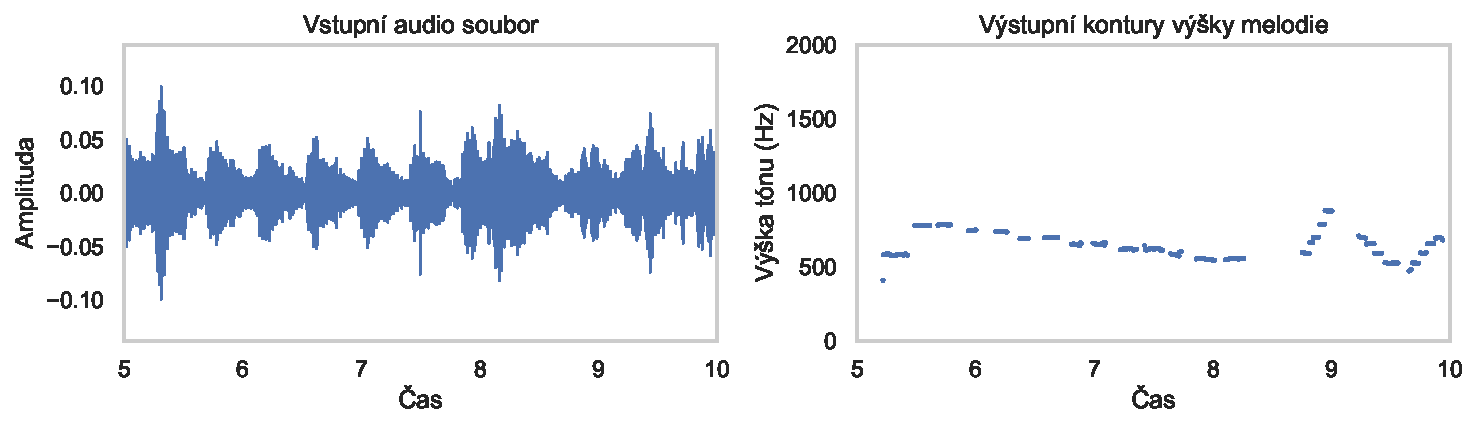
\includegraphics[width=\textwidth,height=\textheight,keepaspectratio]{../img/input_output}
\caption{Příklad vstupu a výstupu metody pro extrakci melodie. \textcolor{red}{přidat zvukový přílkad do přílohy}}
\label{obr:input_output}
\end{figure}

Tato práce se zabývá metodami odhadu fundamentální frekvence melodie ze zvukové nahrávky. Jinými slovy je naším cílem získat v každém bodě vstupní skladby informaci o tom, zda melodie v daném okamžiku zní a její případnou výšku. Jde o jednu z nejdůležitějších a zároveň nejtěžších úloh z oboru \textit{Music Information Retrieval} (MIR), jejíž rozsah využití v této doméně pokrývá významnou část aktivně řešených, otevřených problémů. 

Spolehlivý přepis melodie by usnadnil vyhledávání v hudebních datech, ať už na základě notového zápisu (\textit{Symbolic Melodic Similarity}), pomocí nekvalitní nahrávky z rádia (\textit{Audio Fingerprinting}), pomocí broukání (\textit{Query by Singing/Humming}) nebo dokonce pomocí coveru hledané písně (\textit{Audio Cover Song Identification}). Mimo vyhledávání by byl algoritmus užitečný pro další zpracování zvukového signálu, ať už pro manipulaci a úpravu melodického hlasu (například software Melodyne), nebo naopak jeho odstranění a vytvoření karaoke doprovodu (\textit{Informed Source Separation}). V neposlední řadě by extrakce melodie pomohla při kategorizaci hudebních dat, například podle žánru (\textit{Genre Classification}) nebo podle zpěváka (\textit{Singer Characterization}). A konečně široké spektrum využití by nalezla i v muzikologii (případně etnomuzikologii) pro kvantitativní i kvalitativní studii hudebních motivů a postupů (V jazzu například \cite{Pfleiderer}).

Extrakce melodie však nemusí sloužit pouze jako mezikrok pro řešení jiné úlohy, užitečný je i samotný výstup algoritmu, znázorněný na obrázku \ref{obr:input_output}. Motivačním příkladem použití může být pomoc při transkripci. Představíme-li si začínajícího hráče na saxofon, který si chce do not přepsat své oblíbené jazzové sólo, výstup algoritmu mu dá užitečnou informaci o tom, jaký tón zní v jakou chvíli. Z této reprezentace už pak hráči zbývá nalezené tóny projít a zapsat je do notové osnovy.

\section{Analýza hudebního signálu}

Proč je ale extrakce melodie otevřený problém? Příbuzná úloha, která spočívá v přepisu nahrávky jednoho izolovaného nástroje, je v podstatě vyřešena \citep{Mauch2014a}, proč se tato úloha po přidání hudebního doprovodu stává výrazně obtížnější? Pro vysvětlení zásadního problému, který se s přepisem nahrávky pojí, musíme nejdříve přiblížit vůbec povahu zvuku a možnosti jeho zkoumání.

Naše zkušenost se zvukem probíhá primárně skrze sluch. Teprve na hlasitém koncertu však člověk pocítí, že zvuk je ve své fyzikální podstatě změna tlaku vzduchu, putující od zdroje k posluchači. Díky sluchu z těchto vibrací dokážeme oddělit jednotlivé zdroje a identifikovat v nich i velmi jemné rozdíly. Ačkoli jde o subjektivní vjemy, zvuky lze částečně rozřadit podle toho, jak snadno v nich rozeznáme nějakou konkrétní výšku. 

\vspace*{0.5cm}

Čtenář této práce si nyní může postupně vybavit: hrající violoncello, odbíjení kostelního zvonu, cinknutí příboru, štěkot psa, plynutí potoka, šelest listí stromů, trhání papíru, tlesknutí a prasknutí balónku.

\vspace*{0.5cm}

Se ztrácející se zřetelností výšky nejprve přijdeme o možnost zpívat společně se zdrojem zvuku v harmonii a posléze i o možnost si představit \uv{vyšší} a \uv{nižší} instance toho samého zvuku (jak zní vysoké a nízké prasknutí balónku?). To, co mají první z uvedených příkladů společné, je výrazná a stabilní periodicita jejich signálu --- daný tlakový průběh se opakuje v čase. Díky sluchu tuto periodicitu interpretujeme jako výšku, přičemž různé výšky se od sebe liší frekvencí, se kterou se signál opakuje. Hudební nástroje jsou jedním ze zdrojů těchto pravidelných vibrací, jejichž frekvenci lze zpravidla měnit (pomocí klapek, pohybu prstu po struně, atd.). Hlas nástroje však není charakteristický pouze svou výškou, nýbrž i barvou. Ta je určena podobou signálu v rámci jedné periody. 

\begin{figure}[h]\centering
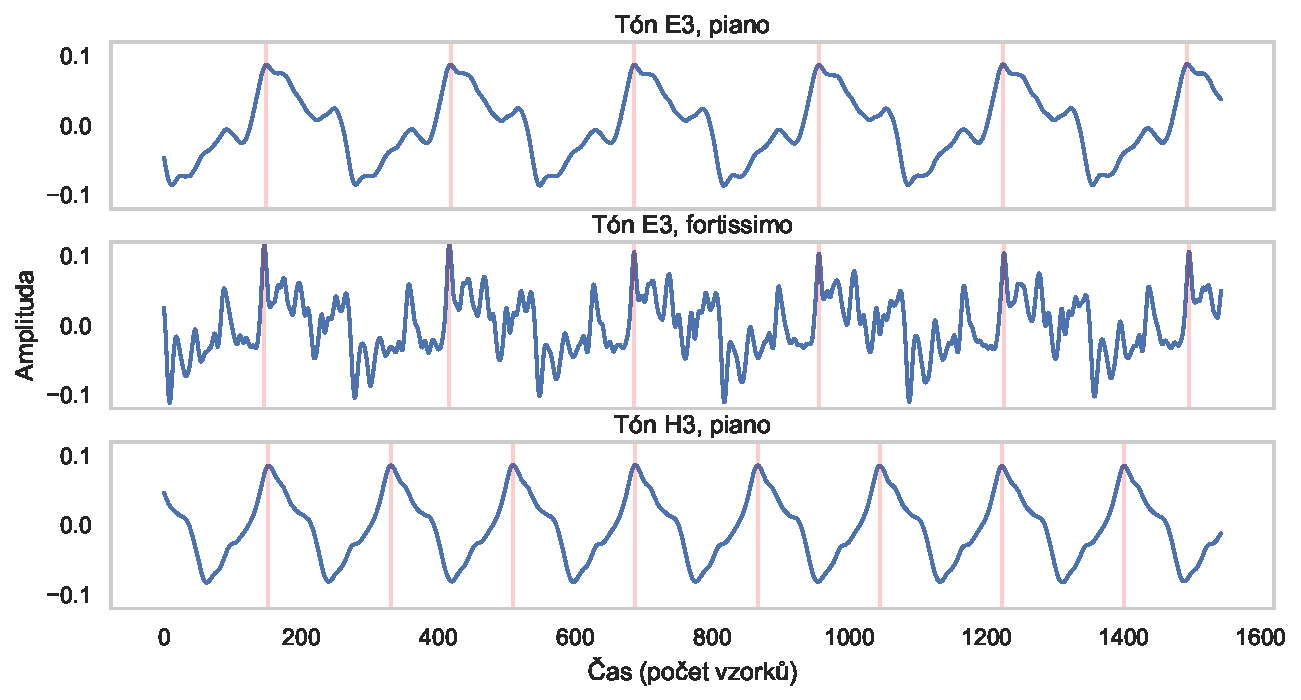
\includegraphics[width=\textwidth,height=\textheight,keepaspectratio]{../img/audio_clarinet}
\caption{Zvuk klarinetu, tóny s různou výškou a dynamikou, 35 milisekund signálu se vzorkovací frekvencí $44\,100\,\rm Hz$. \textcolor{red}{nějak uvést zdroj zvuku \url{https://www.philharmonia.co.uk/explore/sound_samples/clarinet?p=3}}}
\label{obr:audio_clarinet}
\end{figure}

Na obrázku \ref{obr:audio_clarinet} můžeme srovnat tři tóny hrané klarinetem, první dva mají stejnou výšku, jsou ale zahrané s různou intenzitou (dynamikou) \textcolor{red}{je tohle správně formulované, vím že dynamika není intenzita, ale \uv{zahrané s různou dynamikou} mi zní divně?}. Jejich vizuální rozdíl částečně odpovídá i rozdílu v barvě tónu, první tón má příjemný, měkký zvuk; druhý je výraznější a hrubší. Třetí tón se od zbylých liší svou výškou, což lze pozorovat na kratší periodě signálu, která je na obrázku vyznačená úsečkami. 

\begin{figure}[h]\centering
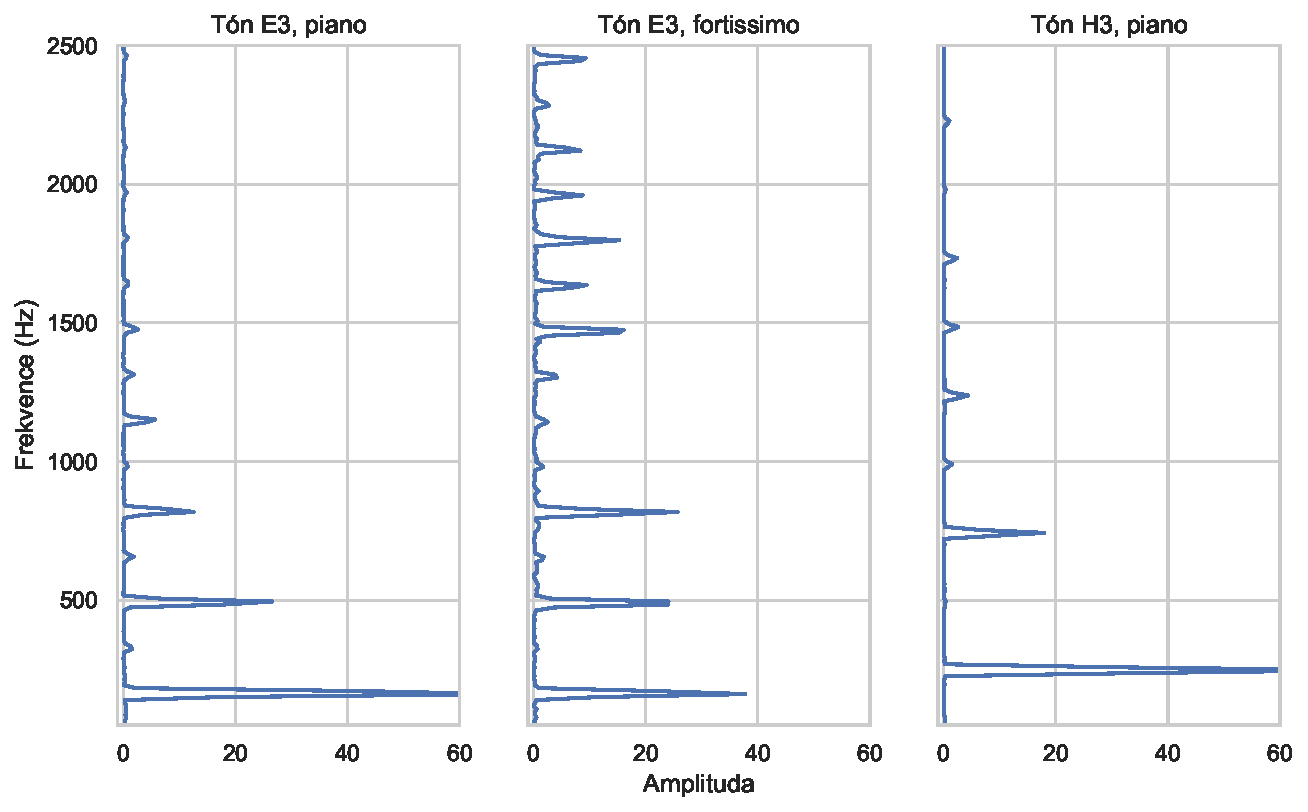
\includegraphics[width=\textwidth,height=\textheight,keepaspectratio]{../img/audio_clarinet_dft}
\caption{Zvuk klarinetu, absolutní hodnota výstupu Fourierovy tranformace signálu délky 4096 s oknem typu Hamming.}
\label{obr:audio_clarinet_dft}
\end{figure}

Jedním ze způsobů analýzy zvukového signálu je pomocí Fourierovy transformace (DFT). Základní myšlenkou je, že na signál lze hledět jako na vážený součet jednodušších signálů. Podobně, jako když se barvy na obrazovce míchají ze tří základních, libovolný zvuk můžeme smíchat ze sady sinusoid. Výslednou kombinaci všech frekvencí, ze kterých se zvuk skládá, označujeme \emph{zvukové spektrum}. Na obrázku \ref{obr:audio_clarinet_dft} vidíme část výsledku Fourierovy transformace zvuků klarinetu z předchozího příkladu. To zásadní, co na spektru tónu můžeme pozorovat, je jeho podstata jakožto součet \emph{harmonických složek}. Tón, kterému posluchač přisoudí výšku $f_0$, se zpravidla skládá ze součtu sinusoid, jejichž frekvence je celočíselným násobkem základní frekvence $f_0$ (jinak také nazývaná \emph{fundamentální frekvence}). Například tedy tón E3 se na obrázku \ref{obr:audio_clarinet_dft} skládá ze složek o frekvenci $165\,\rm Hz$, $330\,\rm Hz$, $495\,\rm Hz$, \dots, zároveň intenzita těchto harmonických frekvencí určuje barvu hlasu.

Ukazuje se, že práce s touto reprezentací zvuku je pro analýzu signálu užitečnější, než práce s nezpracovaným signálem. Ze spektrální reprezentace je například na první pohled zřejmý vztah fundamentálních frekvencí porovnávaných signálů, který odpovídá lidské intuici o výšce zvuků --- tón H3 je na obrázku \ref{obr:audio_clarinet_dft} opravdu \uv{výše} než tón E3. Díky spektrální analýze lze také pozorovat charakteristiky hlasů různých nástrojů. Pro hlas klarinetu platí, že liché harmonické frekvence jsou mnohem výraznější než sudé (na obrázku \ref{obr:audio_clarinet_dft} vypadají sudé harmonické jako malé vrcholky mezi výraznými lichými), naopak například lidský zpěv je charakteristický výraznějšími sudými harmonickými složkami. Další výhodou je možnost hledání rozdílů v barvě tónů --- na spektru vidíme, že vyšší harmonické jsou u tónu hraném fortissimo mnohem výraznější než u tónu hraném piano. Tyto vyšší frekvence způsobují zmiňovanou hrubost tónu. \textcolor{red}{a tohle se dá říct? Tón hraný fortissimo/piano. Moje znalosti hudební terminologie jsou nulové}

Harmonická struktura, která je vlastní lidskému hlasu a téměř všem zvukům hudebních nástrojů, je zásadní pro metody extrakce melodie. Je to vlastnost, která zvuky potenciálně nesoucí melodii odlišuje od bubnového doprovodu, od šumu nebo od jiných nemelodických rušení. Díky ní se také můžeme pokoušet rozložit souzvuk různě vysokých tónů na jejich původní, čisté signály. 

\textcolor{red}{spektrogram hudby - basa, zpěv a bubny. Pod tím obrázek kompletního přepisu melodických kontur}

\begin{figure}[h]\centering
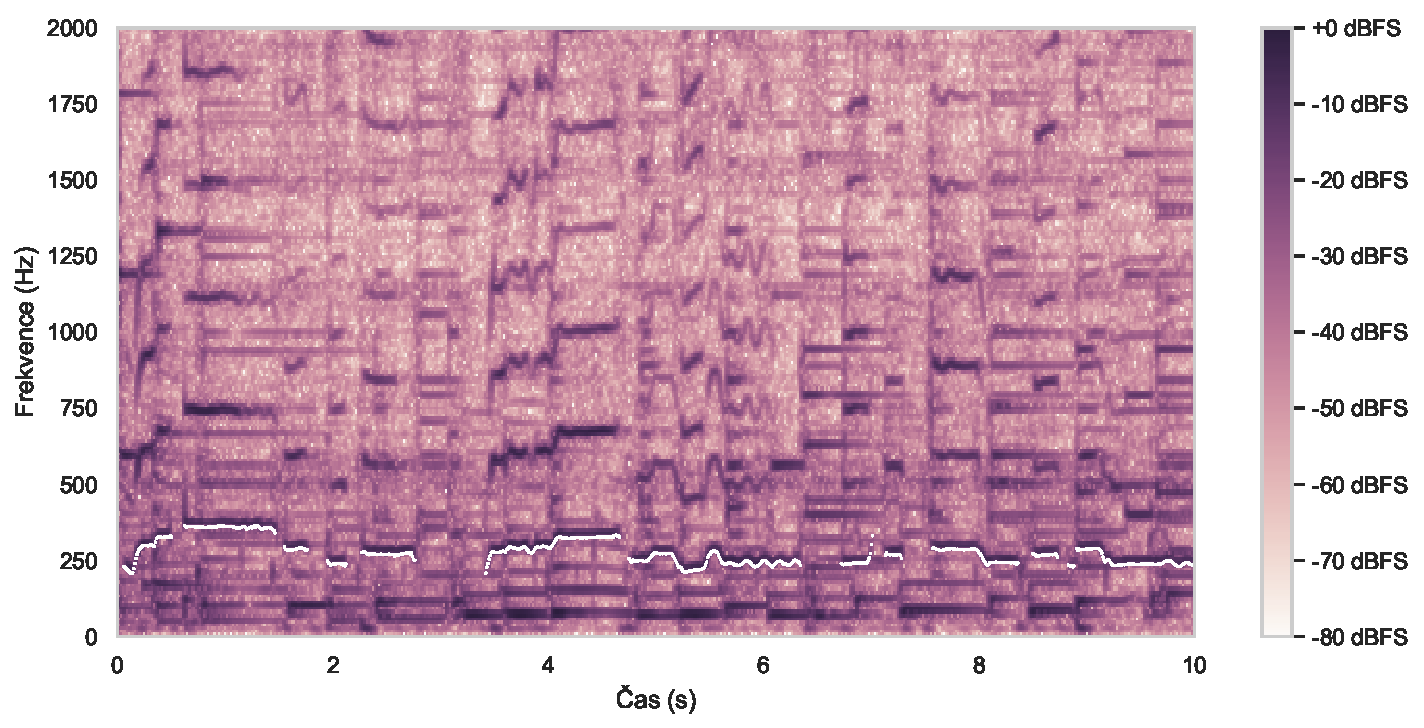
\includegraphics[width=\textwidth,height=\textheight,keepaspectratio]{../img/audio_mix_stft}
\caption{Spektrogram zpěvu s doprovodem piana, basy a perkusí; zpívaná melodie je vyznačena bílým obrysem.}
\label{obr:audio_mix_stft}
\end{figure}

Obrázek \ref{obr:audio_mix_stft} vznikl pomocí opakované Fourierovy transformace, která byla aplikována na po sobě jdoucí, krátké časové úseky vstupní nahrávky, přičemž intenzity frekvenčních složek v každém časovém okamžiku zvuku jsou nyní znázorněny odstínem barvy. Časově-frekvenční reprezentaci signálu nazýváme obecně \emph{spektrogram}, a jeho výpočet je prvním krokem většiny metod pro extrakci melodie.

Na spektrogramu \ref{obr:audio_mix_stft} můžeme pozorovat harmonické struktury tónů --- vyznačenou konturu hlasu, která se na frekvenční ose pohybuje volněji, a pak klavírní a basový doprovod, charakteristický frekvenční stabilitou a v čase slábnoucí amplitudou. Na tomto jednoduchém příkladu lze melodii zpozorovat poměrně snadno, nese ji velmi výrazný, v poměru k doprovodu nejsilnější hlas. Lze na něm však prezentovat první ze základních problémů extrakce melodie.

Frekvence tónů, ze kterých se skládá hudební skladba, jsou uspořádány do stupnic, které definují pevně dané poměry (hudební \emph{intervaly}), ve kterých se tyto tóny ve skladbě mohou vyskytovat. Principem libozvučnosti jsou však takové intervaly, které způsobují, že harmonické frekvence jednotlivých tónů se překrývají a ve výsledné směsi pak není zřejmé, zda-li daná harmonická frekvence patří k jednomu, či více hlasů. Hudební doprovod, pro lidské ucho znějící \uv{pod melodií}, tedy často svými harmonickými frekvencemi zasahuje do melodie samotné, což je zřejmé ze spektrální analýzy.

Dekompozice signálu na jednotlivé znějící hlasy, která je pro člověka přirozená podobně, jako porozumění řeči v rušné kavárně, se kvůli této harmonické povaze tónů a intervalů stává pro algoritmy extrakce melodie obtížným problémem. To, co pro nás činí hudbu zajímavou pro poslech, ji činí obtížně analyzovatelnou pro počítač.


% * další nepříjemnosti
%     * rezonance nástroje po zahrání tónu
%     * dozvuk místnosti
%     * rušení z perkusí
%     * mastering = sice je nahrávka více vyrovnaná, ale problémy přepisu ještě zesiluje
%         * digitální reverb (= dále rozostřuje hranice mezi začátky a konci not, zvětšuje míru překryvů zahraných not)
%         * dynamic range compression = komprese dynamiky zvukového signálu = zmenšuje rozdíly mezi tichými a hlasitými zdroji zvuku
%             * Komprese dynamiky zvukového signálu je proces používaný v audiotechnice ke zmenšení dynamického rozsahu zpracovávaného signálu

\begin{figure}[h]\centering
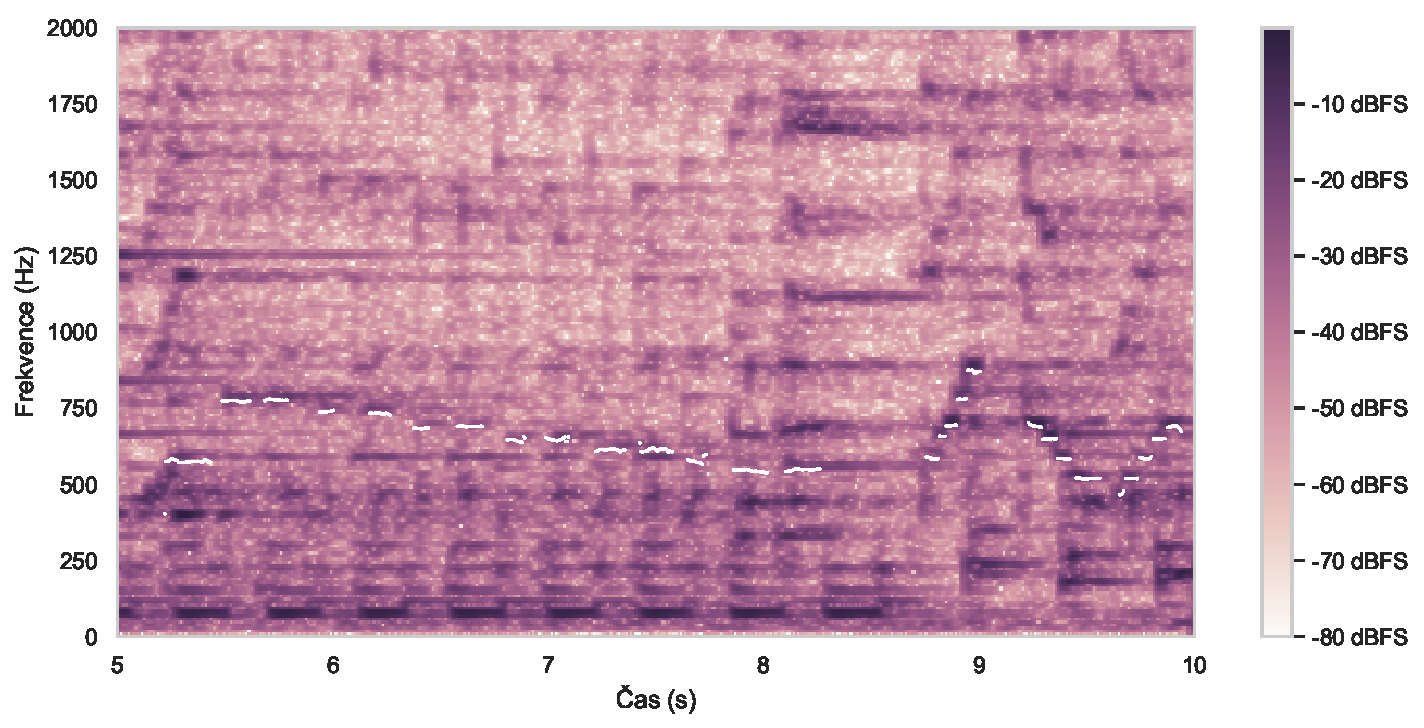
\includegraphics[width=\textwidth,height=\textheight,keepaspectratio]{../img/audio_mix_stft_2}
\caption{Spektrogram orchestrální skladby s obtížně detekovatelnou melodií.}
\label{obr:audio_mix_stft_2}
\end{figure}

\section{Definice melodie}

Rozpoznání melodie v rámci hudební skladby je pro většinu posluchačů intuitivní schopností, která je součástí prožitku poslechu hudby, a která jejímu poslechu vůbec dává smysl. Ačkoli je melodie tedy termín, který je subjektivně jasný, formální, obecně přijímanou muzikologickou definici, která by se zpětně neodkazovala k posluchači, nemá. 

Z tohoto důvodu si výzkumné týmy zabývající se automatickou transkripcí melodie volí pragmaticky spíše užší definice melodie, se kterými se v jejich kontextu pracuje lépe. Práce \cite{Goto1999}, která je považována za jednu z prvních prací v oboru, chápe melodii jako \uv{konturu fundamentální frekvence sestávající se z nejsilnějších tónů hrajících v omezeném frekvenčním rozsahu}. Práce se tedy omezuje na poměrně úzké chápání melodie, obecně se totiž tóny melodie jistě mohou vyskytovat i mimo autory specifikovaný frekvenční rozsah a také nemusí být vždy v poměru s doprovodem nejhlasitější složkou signálu. Z technického hlediska však umožnila autorům implementaci algoritmu běžícího v reálném čase, který poskytoval sémanticky bohatý popis vstupních nahrávek. Navazující články již pracují s volnějšími definicemi, které lépe reflektují podstatu melodie. 

Kompromisem mezi subjektivní a praktickou definicí se na dlouhou dobu stala \uv{extrakce základní frekvence hlavního, neměnného, melodického hlasu}. Ačkoli melodii v reálném hudebním materiálu obvykle nese více hlasů, které se v hraní střídají (například píseň se zpěvem a kytarovým sólem), v letech 2005 -- 2015 se v soutěži MIREX (mezinárodní soutěž pro metody řešící MIR úlohy) provádí evaluace pouze nad krátkými výňatky, kde tato definice není omezující. Přestože se může na první pohled zdát, že tato definice pouze uměle zjednodušuje celou úlohu, její formulace vede k rozvoji nových a zajímavých přístupů, které se sice formálně soustředí právě na extrakci pouze jednoho neměnného hlasu, ale ve výsledku překvapivě dobře fungují i na složitější skladby. Příkladem nového směru může být extrakce melodie pomocí modelování hudebního záznamu jako součtu signálu jednoho hlasu a doprovodu (práce \cite{Durrieu2010} nebo \cite{Bosch2016b}) s přesahem do příbuzné úlohy oddělení hlasů (source separation). Některé práce se zaměřují ještě konkrétněji na separaci lidského zpěvu a doprovodu (\cite{Hsu2010}, \cite{Ikemiya2016}). Nově se také objevují práce, které \uv{hlavní} melodický hlas neinterpretují nutně jako \uv{nejsilnější} a k jeho rozlišení využívají dalších rysů, jako je barva, vibrato nebo délka not. Například \cite{Salamon2012a} využívají těchto rysů pro finální výběr mezi extrahovanými kandidátními konturami.

Ve svém přehledovém článku \cite{Salamon2014} dochází k závěru že výzkum začal v letech 2009--2012 stagnovat, nová data jsou proto pro další vývoj oboru zásadní. Výrazným posunem v rámci MIR komunity proto bylo zveřejnění nových datasetů MedleyDB \citep{Bittner2014} a ORCHSET \citep{Bosch2016}, oba obsahují data, ve kterých již melodii nenese pouze jeden hlas po celou dobu skladby. V porovnání s do té doby dostupnými daty jde také o mnohem rozmanitější kolekce a v případě MedleyDB jde o první volně dostupný dataset, ve kterém se objevují celé skladby, nikoli pouze výňatky.

\cite{Bosch2016} pro práci na datasetu ORCHSET definuje melodii jako \uv{jednohlasou sekvenci tónů, kterou bude posluchač nejspíše reprodukovat, pokud jej požádáme o zapískání či zabroukání příslušné skladby} (na základě článku \cite{Poliner2007}), pro sestavení kolekce dat proto opravdu využívá skupiny posluchačů, které po poslechu krátkých ukázek orchestrální hudby následně žádá o přezpívání melodie. V případě MedleyDB se na anotacích melodie podílí skupina profesionálních hudebníků a vznikají tři různé přepisy melodie s různě volnými formulacemi definice melodie.

Celkový směr výzkumu je tak ve výsledku velmi podmíněn dostupnými daty. Ta tvoří jakýsi protipól k ryze technickým a objektivním cílům algoritmických metod. Nadějí je, že tato dialektika vývoje algoritmů a práce na datech vyústí jednak v metody extrakce, které věrně zachycují podstatu subjektivního prožitku porozumění hudbě, a jednak v celkovém důsledku také snad v lepší porozumění pojmu melodie obecně.

\section{Metody extrakce melodie}

\begin{figure}[h]\centering
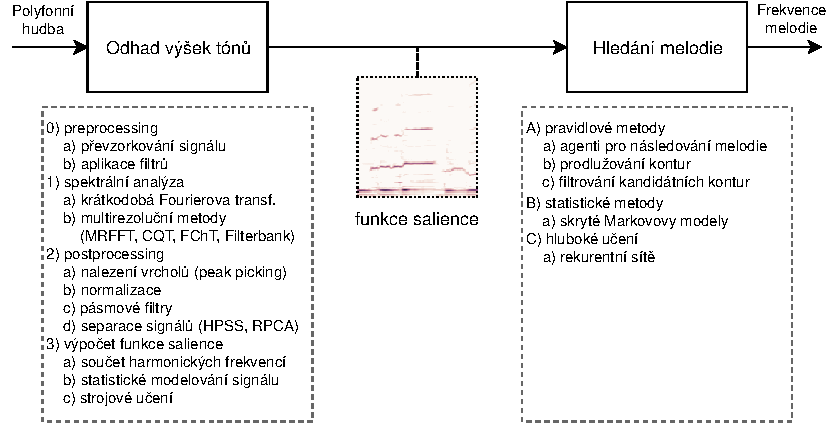
\includegraphics[width=\textwidth,height=\textheight,keepaspectratio]{../img/diagram_systemy_ME}
\caption{Diagram obvyklého návrhu metod pro extrakci melodie.}
\label{obr:diagram_systemy_ME}
\end{figure}

Základním a společným přístupem k problému extrakce melodie je dekompozice na podproblémy odhadu výšek všech znějících hlasů v signálu a následného výběru melodické linie z těchto kandidátních kontur. Jednotlivé metody se pak liší ve způsobech řešení těchto podproblémů, mimo jiné také v míře abstrakce od původního signálu, které při zpracovávání dosahují --- zatímco některé přístupy po celou dobu pracují pouze se signálem jako takovým a důmyslnými způsoby ho transformují tak, aby získaly co nejpřesnější odhad výšky melodie, jiné metody při výpočtu vytváří symbolický popis jednotlivých not a následně i celých frází a melodii pak hledají v tomto vysokoúrovňovém popisu nahrávky. Shrnutí používaných přístupů, blíže popsaných v kapitole \hyperref[chap:souvisejici]{Související práce}, můžeme vidět na diagramu \ref{obr:diagram_systemy_ME}.

\begin{figure}[h]\centering
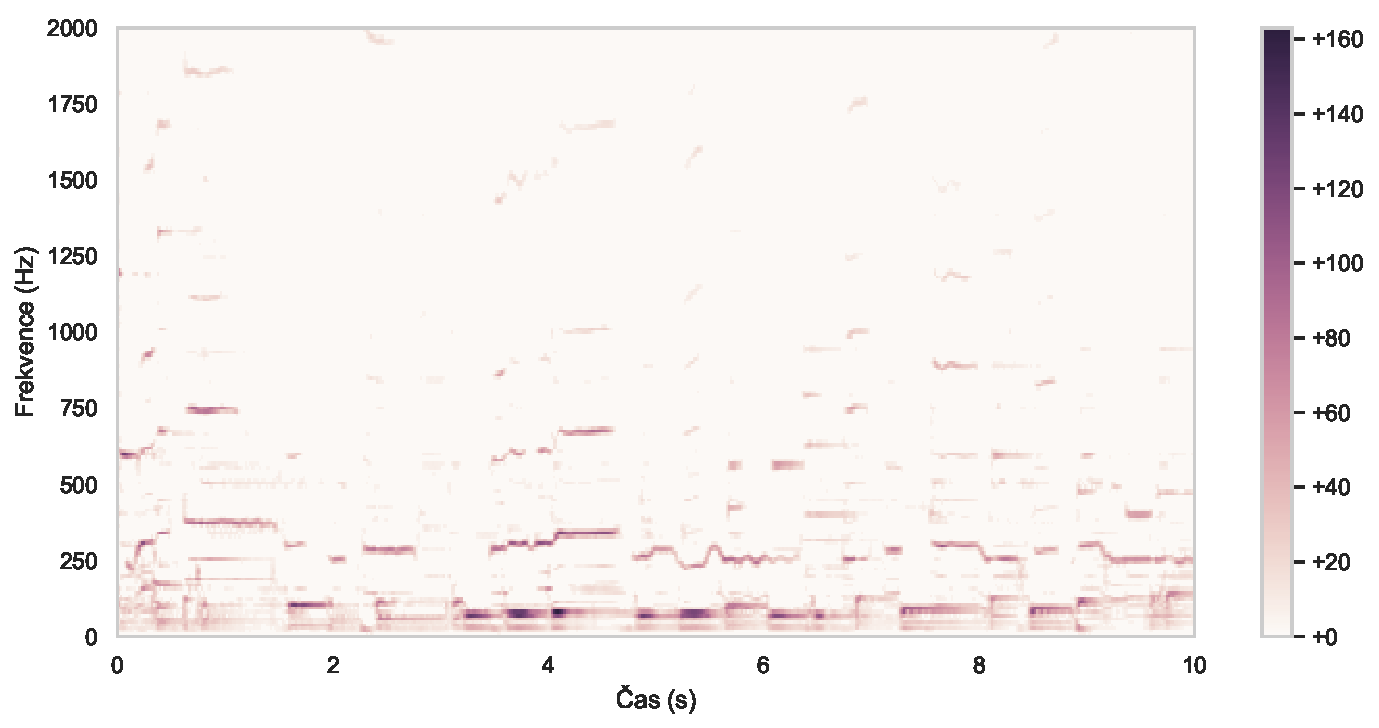
\includegraphics[width=\textwidth,height=\textheight,keepaspectratio]{../img/salience}
\caption{Příklad výstupu výpočtu salienční funkce pomocí váženého sčítání harmonických frekvencí. Ačkoli je zpěv velmi zvýrazněn a salienční funkce na většině nahrávky dobře zachycuje výšku znějící melodie, doprovod kolem čtvrté sekundy nahrávky má vyšší hodnotu než zpěv, což neodpovídá lidskému vnímání zpěvu jakožto nejdůležitější složky signálu.}
\label{obr:salience}
\end{figure}

Prvním krokem všech existujících metod pro extrakci melodie je převod zvukového signálu do frekvenční domény, ať už pomocí zmiňované STFT nebo použitím jiných metod vyvinutých pro analýzu harmonického signálu (MRFFT, CQT, FChT, \dots). Jednou z hlavních výhod těchto dalších metod je logaritmická osa frekvence, díky které je snadné pracovat s harmonickými poměry a hudebními intervaly nezávislé na výšce frekvence. Abychom tuto vlastnost ilustrovali, uvedeme příklad --- tóny A4 a E5 jsou vzdálené o kvintu (na klavíru od tónu A4 musíme postupně zmáčknout 7 bílých a černých klapek, abychom se dostali k tónu E5), tóny A5 a E6 jsou také vzdálené o kvintu. Rozdíl frekvencí těchto tónů je však $220\,\rm Hz$ mezi první dvojicí a $440\,\rm Hz$ mezi druhou dvojicí, tudíž vzdálenost frekvencí daného intervalu závisí na tónu, od kterého se tento interval počítá. Protože je hudební interval jistý \emph{poměr} mezi dvěma tóny, použitím logaritmické osy frekvence se tyto poměry budou jevit jako absolutní rozdíly ($\log n f_0 = \log n + \log f_0$). 

Zpracováním spektrogramu vstupu pak vzniká tzv. \emph{funkce salience}, která každé znějící frekvenci v signálu přiřazuje jisté ohodnocení, které vyjadřuje poměrnou důležitost dané frekvence k ostatním slyšitelným složkám. Funkce salience je tedy v jistém slova smyslu speciální frekvenčně-časová transformace, která podává zejména informace o znějící melodii, nikoli o celkové kompozici signálu. Na obrázku \ref{obr:salience} můžeme srovnat funkci salience vypočtenou pomocí váženého součtu harmonických frekvencí se vstupním spektrogramem \ref{obr:audio_mix_stft}.

Druhým krokem je pak výběr melodie na základě funkce salience. Triviálním řešením je výběr takových frekvencí, které mají nejvyšší ohodnocení. Problémem tohoto přístupu je však to, že jakmile signál obsahuje více podobně ohodnocených tónů, výstup tohoto řešení má tendenci mezi těmito kandidáty často \uv{přeskakovat}. Algoritmy pro extrakci melodie proto volí různě pokročilé metody vyhlazování, případně metody hledání nejpravděpodobnějšího průchodu posloupností stavů (například pomocí Viterbiho algoritmu).

\section{Hluboké učení}

Motivací pro použití metod strojového učení je překonání limitů člověkem navržených, rigidních, pravidlových systémů. Cílem je automatické nalezení optimálního postupu pro řešení úlohy, na základě množství dat, ve kterých strojové učení dokáže nalézt a využít jejich pravidelností. V našem případě pak po metodě založené na strojovém učení požadujeme, aby na základě příkladů z trénovací množiny vytvořila funkci salience.

Výhodou tohoto přístupu je, že o vstupních datech nemusíme dělat žádné předpoklady. Vzniklá metoda pak může v praxi zohledňovat více faktorů ovlivňujících přítomnost melodie, jako je její barva, frekvenční modulace (vibrato, glissando) nebo hlubší vzájemné srovnání současně znějících tónů. Na základě trénovacích příkladů může být tato metoda robustnější vůči většímu spektru barev hlasů nástrojů --- zatímco předešlé metody pro extrakci melodie často uvažují signály s postupně se snižujícím podílem harmonických frekvencí, opravdové signály hudebních nástrojů často tento předpoklad nesplňují (viz obrázek \ref{obr:audio_clarinet_dft}).

První pokus o využití těchto metod představili \cite{Poliner}, vstupní signál transformovali pomocí krátkodobé Fourierovy transformace a část spektra po jednoduché normalizaci použili jako vstupní data pro metodu podpůrných vektorů (SVM). Jejich metoda měla své limitace, výstup byl kvantizován na úroveň jednoho půltónu a tudíž metoda nedokázala dobře postihnout například vibrata. I přesto však tým dosáhl srovnatelných výsledků s ostatními metodami. 

Po roce 2005 jakékoli pokusy o aplikaci strojového učení ustávají a na nové metody se čeká až do roku 2016, jedním z důvodů byl jistě nedostatek dat, tuto situaci zlepšil například dataset MedleyDB \citep{Bittner2014} nebo dnes již zaniklý iKala \citep{Chan2015}. Zájem o strojové učení však znovu stoupá, také díky úspěšnému využití hlubokých neuronových sítí napříč ostatními obory. Na konferenci ISMIR 2016\footnote{International Society for Music Information Retrieval Conference} objevují dva články týmů \cite{Kum2016} a \cite{Rigaud2016}, založené právě na hlubokém učení. V roce 2017 publikuje své metody \cite{Bittner2017} (ISMIR), \cite{Balke2017} (ICASSP\footnote{International Conference on Acoustics, Speech, and Signal Processing}), následující rok přináší metody \cite{DBasaranSEssid2018} (ISMIR), \cite{Bittner2018}. Všechny zmíněné popisujeme v kapitole \hyperref[chap:souvisejici]{Související práce}. V oboru lze tedy od roku 2016 vidět velmi výrazný trend právě směrem k hlubokému učení, a stejný směr je patrný i v příbuzných úlohách přepisu hudby. Tým z laboratoře Google Brain dokázal výrazně zlepšit přepis klavírních skladeb pomocí kombinace konvoluční a rekurentní architektury \citep{Hawthorne2018}. Neuronové sítě také zlepšují výsledky na poli oddělení signálů \citep{Stoller2018}.

V této práci se pokusíme navázat na zmiňované práce a otestovat nové architektury hlubokých neuronových sítí pro úlohu extrakce melodie, zejména pak pro hledání nových způsobů výpočtu funkce salience, v menší míře také pro detekci melodie.

\section{Přínosy práce}

\textcolor{red}{TODO}

\section{Struktura práce}

\textcolor{red}{napsat signpost}

% \cite{Thickstun2016} - musicnet
% \cite{Hawthorne2018} - google magenta

% V oboru transkripce hudby se trend v použití hlubokých sítí
\chapter{Související práce}

\section{Definice melodie}


Jelikož z muzikologického hlediska žádná jasná a obecně přijímaná definice melodie neexistuje a ve výsledku melodie zůstává pro každého posluchače ryze subjektivním pojmem, pro extrakci melodie si výzkumné týmy volí spíše pragmaticky takové definice, se kterými se nejlépe pracuje. Příkladem může být jedna z prvních prací zabývající se extrakcí melodie. Výstupem v práci \cite{Goto1999} je kontura fundamentální frekvence sestávající se z nejsilnějších tónů hrajících v omezeném frekvenčním rozsahu. Tato definice je poměrně úzká, tóny melodie se totiž jistě mohou vyskytovat i mimo autory specifikovaný rozsah a nemusí být vždy v poměru s doprovodem nejsilnější složkou signálu. Z technického hlediska však umožnila autorům implementaci algoritmu běžícího v reálném čase, který poskytoval sémanticky bohatý popis vstupních nahrávek. Navazující články pracují s volnějšími definicemi, které lépe reflektují podstatu melodie. Mimo to se používaná definice proměňuje díky novým datasetům, jejichž autoři tvoří protipól k ryze technickým a objektivním cílům algoritmických metod. Zatímco pro tvorbu algoritmů je praktické zvolit co nejkonkrétnější cíl, při tvorbě datasetu se naopak projevuje lidská subjektivita autorů anotací. 

Kompromisem mezi subjektivní a praktickou definicí se na dlouhou dobu stala \uv{extrakce základní frekvence hlavního melodického hlasu}. Ačkoli melodii v reálném hudebním materiálu obvykle nese více hlasů, které se v hraní střídají (například píseň se zpěvem a kytarovým sólem), v letech 2005 -- 2015 se v soutěži MIREX provádí evaluace pouze nad krátkými výňatky, kde tato definice není omezující. Tento pohled však otevírá také jiné přístupy, například extrakci melodie pomocí modelování hudebního záznamu jako součtu signálu jednoho hlasu a doprovodu \citep{Durrieu2010}, \citep{Bosch2016b} nebo přímo omezení se na separaci lidského zpěvu a doprovodu \citep{Ikemiya2016}. Nově se objevují práce, které \uv{hlavní} melodický hlas neinterpretují nutně jako \uv{nejsilnější}. Skladatelé a hráči používají množství různých postupů, které melodii zvýrazňují --- krom dynamiky ji ovlivňuje například také barva hlasu, vibrato nebo délka not. \cite{Salamon2012a} využívá těchto rysů pro výběr mezi kandidáty na melodickou konturu.

Posunem v rámci MIR komunity bylo zveřejnění nových datasetů MedleyDB \citep{Bittner2014} a ORCHSET \citep{Bosch2016}, oba přináší nová data, ve kterých již melodii nenese pouze jeden hlas po celou dobu skladby. V porovnání s do té doby dostupnými daty jde o mnohem rozmanitější kolekce. V případě MedleyDB jde o první volně dostupný dataset, ve kterém se objevují celé skladby, nikoli pouze výňatky a autoři předkládají rovnou tři verze anotací:

\begin{enumerate}
    \item Základní frekvence nejvýraznějšího melodického hlasu, jehož zdroj zůstává po dobu nahrávky neměnný.
    \item Základní frekvence nejvýraznějšího melodického hlasu, jehož zdroje se mohou měnit.
    \item Základní frekvence všech melodických hlasů, potenciálně pocházejících z více zdrojů.
\end{enumerate}

První formulace je v souladu s doposud používanou definicí. Zbylé dvě se snaží posouvat možné cíle budoucích metod a předložit komunitě nové výzvy, podle \cite{Salamon2014} totiž výzkum začal v letech 2009--2012 stagnovat. Zatímco anotace s jednou melodickou linkou (1. a 2. definice) se v navazujících pracích často používají, zatím žádný článek se nepokusil představit metodu, jejímž cílem by bylo extrahovat více melodických linek (3. definice).

\cite{Bosch2016} při práci na datasetu ORCHSET vychází z článku \cite{Poliner2007}, který definuje melodii jako \uv{jednohlasou sekvenci tónů, kterou bude posluchač nejspíše reprodukovat, pokud jej požádáme o zapískání či zabroukání příslušné skladby}. Přestože nejde o objektivní definici, v praxi se posluchači často na jedné konkrétní sekvenci tónů shodnou, a to jak u populární hudby, kde melodii často nese lidský zpěv, tak u orchestrálních skladeb. Ačkoli se definice neujala pro metody extrakce, \cite{Bosch2016} ji využili pro anotaci výňatků z orchestrálních skladeb, u kterých by předchozí zmíněné definice selhávaly, jelikož pojem melodie je u orchestrální hudby mnohdy komplikovanější než u jiných žánrů. Anotace tak spočívala v přezpívání orchestrálních výňatků skupinou posluchačů a následném srovnání a zpracování těchto nahrávek.

\section{Průzkum existujících metod}

Jen do soutěže MIREX se od roku 2005 přihlásilo 45 týmů s 62 různými metodami pro extrakci melodie, s různou mírou přesnosti přepisu. Mezi přístupy k tomuto problému tedy existuje veliká rozmanitost, jejíž kompletní popis přesahuje rámec této práce. Zaměříme se proto na společné rysy a celkové trendy v oboru. 

Shrnující práce od \cite{Poliner2007} a \cite{Salamon2014} se pro charakterizaci systémů pro transkripci odkazují na příbuznou úlohu odhadu fundamentální frekvence monfonní nahrávky. Algoritmy pro monofonní tracking na základě vstupního signálu $x(t)$ počítají \emph{funkci salience} $S_x(f_\tau, \tau)$ pro každý krátký časový okamžik (okno) $\tau$ a frekvenci $f_\tau$. Výsledkem této funkce je relativní ohodnocení (příp. pravděpodobnost) jednotlivých frekvencí obsažených ve vstupním signálu, které značí, zda-li je daná frekvence fundamentální frekvencí znějícího hlasu. 

Výstupem monofonního trackingu je posloupnost frekvencí s maximální saliencí, tedy posloupnost frekvencí, které jsou nejlépe ohodnocenými kandidáty na fundamentální frekvenci. V praxi se k salienci ještě přičítají temporální závislosti, aby se zajistila kontinuita extrahovaných frekvenčních kontur a zvýšila robustnost proti šumu obsaženému v nahrávce. 

Přejdeme-li k úloze extrakce melodie, obecně se vstupní polyfonní signál $x(t) = x_m(t) + x_d(t)$ skládá ze směsi melodického hlasu $x_m(t)$ a hudebního doprovodu $x_d(t)$, cílem metod pro extrakci je z pohledu přepisu fundamentální frekvence zvýšení robustnosti algoritmu vůči tomuto \uv{melodickému šumu} $x_d(t)$. Výstupem našeho systému tedy bude posloupnost odhadů frekvence v každém časovém okně vstupního signálu, reprezentovaná vektorem $\hat{\mathbf{f}}$:

    $$\hat{\mathbf{f}} = \argmax_{\mathbf{f}}{[\sum_{\tau}{S'_x(f_\tau, \tau)} + C(\mathbf{f})]}$$

kde $f_\tau$ je frekvence na pozici $\tau$ ve vektoru $\mathbf{f}$. $S'_x(f_\tau, \tau)$ je upravená funkce salience, která při výpočtu zohledňuje vliv doprovodu a složka $C(\mathbf{f})$ představuje temporální vlastnosti melodie. 

Spolu s odhadem frekvencí by také měl systém na výstupu určit úseky, ve kterých v nahrávce melodie zní a kdy nikoli. K výstupu tedy patří také vektor $\hat{\mathbf{v}}$, se stejným počtem složek jako $\hat{\mathbf{f}}$, který značí znělost melodie v každém časovém okně $\tau$.

Většina existujících metod sdílí podobnou základní strukturu při řešení extrakce, která se zakládá na popsané formalizaci. Prvním krokem je transformace zvuku do frekvenční domény a následný odhad znějících výšek tónů v polyfonním signálu (výpočet \emph{funkce salience}), druhým krokem je pak zpracování těchto odhadů a výběr melodie (tedy zpřesnění výsledné $\hat{\mathbf{f}}$ pomocí $C(\mathbf{f})$). Přístupy k řešení těchto dvou kroků již s konkrétními příklady nastíníme v dalších sekcích.

\subsection{Odhad výšek tónů}

\subsubsection{Spektrální analýza}

Zvuk hraného tónu na melodickém nástroji je z fyzikálního pohledu periodická změna tlaku vzduchu. Perioda tohoto signálu se nazývá fundamentální frekvence (označujeme F0) a zpravidla je tento signál složen ze součtu řady sinusoid, jejichž frekvence jsou celočíselným násobkem fundamentální frekvence. V čase měnící se amplitudy těchto \emph{harmonických frekvencí} udávají hlasitost a barvu hlasu, výška první harmonické frekvence (tj. výška fundamentální frekvence) pak ve většině případů odpovídá posluchačem vnímané výšce tónu. 

\textcolor{red}{TODO obrázek: signál -> spektrum -> salience}

Prvním krokem metod pracujících s hudebním signálem je proto provedení spektrální analýzy, jde o převod zvuku do frekvenční reprezentace, která odhaluje tyto harmonické struktury tónů a umožňuje s nimi dále pracovat. 

% \subsubsection{Krátkodobá Fourierova transformace}

Přístupů ke spektrální analýze je více, přímočará a podle \cite{Dressler2016} nejčastěji používaná metoda je \emph{krátkodobá Fourierova transformace} (STFT). Jejím principem je rozdělení vstupního signálu na množinu překrývajících se oken konstantní délky a výpočet Fourierovy transformace těchto krátkých zvukových úseků. Komplexní výsledek transformace umocníme a získáme tzv. výkonové spektrum signálu, které obsahuje informaci o poměrech energie frekvencí, ze kterých se signál v okně skládá. 

$$X(f, \tau) = \int_{-W/2}^{W/2}{w(t)y(\tau + t)e^{-j2\pi f t} \mathrm{d}t}$$

Na libovolnou metodu převodu diskretizovaného signálu na frekvenční doménu se inherentně vztahuje Gaborův limit (související s principem neurčitosti). Volbou délky vstupního okna transformace zpřesňujeme buď frekvenční nebo časové rozlišení výsledné spektrální reprezentace. Zvolíme-li krátké vstupní okno, zvyšujeme časové rozlišení (krátké okno lépe zachycuje rychlé změny průběhu signálu), avšak ztrácíme přesnost na frekvenční ose, opačný vztah platí pro volbu delšího okna.

Tato limitace je markatní zejména pokud STFT používáme pro hudební data. Z povahy hudebních intervalů a harmonických struktur tónů platí, že téměř všechny periodické signály se v hudební skladbě vyskytují ve vzájmených relativních poměrech (v případě intervalů v poměrech $2^{\frac{n}{12}}$ a v případě harmonických frekvencí v celočíselných), u vyšších tónů jsou proto rozdíly mezi relevantními frekvencemi absolutně větší než u nižších tónů. Frekvenční rozlišení STFT je konstantní na celém výstupním frekvenčním rozsahu. V praxi proto volba jakékoli velikosti okna zajistí dobrý poměr frekvenčního a časového rozlišení jen pro část rozsahu. Ve výsledku je pak buď pro vyšší frekvence okno příliš velké (zbytečně detailní rozlišení frekvence na úkor časového) a nebo naopak pro nižší frekvence je okno nedostačující (rozlišení frekvence nemusí být ani na úrovni půltónů).

Z tohoto důvodu existují vedle STFT i další metody, jejichž cílem je nabídnout lepší kompromis frekvenčně-časového rozlišení v kontextu melodických dat. \cite{Goto1999} používají MRFFT (Multi-Resolution Fast Fourier Transform), principem je opakovaný downsampling signálu (převzorkování na nižší vzorkovací frekvenci) a aplikace Fourierovy transformace na každý vzniklý signál; s každou iterací spektrum obsahuje čím dál podrobnější informace o nižších frekvencích, protože vyšší frekvence se při downsamplingu ztratí. \cite{Brown1990} popsala metodu Constant-Q Transform (CQT), která spočívá v použití proměnné délky okna Fourierovy transformace pro výstupní frekvenční pásma, která rovnoměrně pokrývají logaritmickou osu frekvence. \cite{Paiva2004} napodobují mechanismy lidského sluchu pomocí banky pásmových filtrů (Cochleagram) s logaritmicky rozmístěnými mezními frekvencemi a sumy autokorelací na jednotlivých frekvenčních pásmech signálu (Summary correlogram).

I přes uvedené důvody se \cite{Salamon2014} a \cite{Dressler2016} domnívají, že metoda zpracování signálu příliš neovlivňuje výslednou přesnost algoritmů pro přepis melodie. Tvrzení dokládají jednak celkovým srovnáním výsledků metod ze všech ročníků soutěže MIREX a jednak neochvějnou převahou využití krátkodobé Fourierovy transformace, jakožto efektivní a dostačující metody pro spektrální analýzu.

\subsubsection{Postprocessing spektrogramu}

Po převodu signálu na frekvenční reprezentaci následuje u většiny metod některý druh úpravy celého spektrogramu, předcházející samotnému výpočtu \emph{funkce salience}. Výsledkem tohoto kroku může být potlačení šumu a nemelodických částí signálu, zpřesnění informace o výšce znějících frekvencí nebo normalizace či jiná úprava amplitud.

Nejčastější úpravou je nalezení lokálních maxim; supresí nemaximálních oblastí se zbavíme velkého množství nemelodických složek signálu, přitom informaci o těch melodických neztratíme. Výhodou práce s množinou maxim je, že jejich frekvenci lze na základě spektra dále zpřesnit pomocí parabolické interpolace (\cite{Rao2010}) a nebo využitím úhlové frekvence (\cite{Salamon2012a}, \cite{Dressler2009}). 

Jinou úpravou jsou různé druhy normalizace, ať jednoduché aplikace logaritmu na jednotlivé hodnoty spektrogramu (\cite{Cancela2008}, \cite{Bittner2017}) nebo složitější strategie normalizace, které závisí na hodnotách celého výsledku Fourierovy transformace jednoho okna (\cite{Ryynanen2008}), či které používají pohyblivé průměry nebo jinou metodu, beroucí v potaz širší zvukový kontext. Cílem normalizace je zvýraznění slabších harmonických frekvencí a potlačení celopásmových zvuků (například perkusí). Principielně podobným krokem je aplikace pásmového filtru (\cite{Goto1999}) pro zvýraznění frekvencí obsahující melodii. Případně využití psychoakustických filtrů modelující lidské vnímání hlasitosti (\cite{Salamon2012a}, \cite{Ikemiya2016}). Ze signálu lze také oddělit melodické nástroje a perkusivní doprovod pomocí metod separace signálů (\emph{source separation}). Používanými metodami jsou například Harmonic/Percussive Sound Separation (HPSS) (\cite{Tachibana2010}) Robust principal component analysis (RPCA) (\cite{Ikemiya2016}).

\subsubsection{Funkce salience}

Salience tónu vyjadřuje míru důležitosti či nápadnosti ke svému hudebnímu okolí. Nejvíce ji ovlivňuje hlasitost v poměru ke zbylým znějícím hlasům, vliv má ale také řada dalších charakteristik hraní. \cite{Dressler2016} mezi příklady uvádí například frekvenční modulaci, jako je vibrato nebo glissando, zejména oproti frekvenčně stálému hudebnímu doprovodu (piano, kytara). Velký vliv má samozřejmě také i barva hlasu. Lidský zpěv nebo obecně zvuky se silnějšími vyššími alikvótními frekvencemi snadněji upoutají pozornost. V případě vícehlasu mají obecně posluchači menší potíže rozeznat výšky tónů na okrajích souzvuku. Pokud má posluchač přiřadit pociťovanou výšku tónu akordu, obvykle volí nejvyšší či nejnižší ze znějících frekvencí.

Výstupem funkce salience pak má být ohodnocení každé výšky tónu v každém časovém okamžiku nahrávky, které co nejlépe odpovídá v relativních poměrech výše popsané zvukové salienci. Jelikož neexistují žádné studie, které by se zabývaly měřením a kvantifikací salience v hudbě, nelze posoudit, jak dobře výsledky obvyklých způsobů výpočtu funkce salience korelují s mírou, ze které vychází. \cite{Bittner2018a} se však domnívá, že odhad bude velmi hrubý, většina postupů totiž do výpočtu zahrnuje pouze hlasitost hlasu, a tedy vynechává řadu jiných důležitých faktorů, které salienci ovlivňují.

Přístupy k výpočtu by se daly zařadit do tří kategorií - sčítání harmonických frekvencí, odhad parametrů modelujících vstup a statistické metody. 

Metody založené na sčítání harmonických frekvencí jsou principiálně nejjednodušší skupinou. Vychází z práce \cite{Hermes1988} a jejich podstatou je využití harmonické struktury zvuku tónů a zpravidla vyšší hlasitosti nejdůležitějšího hlasu. V základní implementaci ohodnocení salience frekvence získáme váženou sumou amplitud všech jejích harmonických frekvencí. Pro spektrogram $X(f, \tau)$ signálu $x$, funkci vah $g(f_\tau, h)$ a $N_h$ počet zahrnutých harmonických frekvencí v sumě:

    $$S'_x(f_\tau, \tau) = \sum_{h=1}^{N_h}{g(f_\tau, h)\abs{X(h \cdot f, \tau)}}$$

Mezi možné rozšíření této základní metody patří například 
    - 

\section{Srovnání existujících metod}

Pro celkové kvantitativní srovnání metod jsme zpracovali 

%     - harmonic summation
%     - ((normalized) subharmonic summation) - vůbec nevim, jak se to liší od HS
%     - joint pitch determination / modeling
%         - source/filter modeling
%     - Fan chirp transform for music representation Cancela
%     - data-based
%         - SVM classifier (Poliner)
%         - Non-negative 
%     - deep models
%         - nejsou nejlépe srovnatelné s ostatními salience funkcemi, protože často mají pro výpočet salience větší kontext než jedno FFT okno
%         - multicolumn deep neural networks \cite{Kum2016}


%  jde zejména o zohlednění frekvenčních charakteristik melodických signálů a metody se liší například ve volbě druhu spektrální transformace signálu

%  společnou základní strukturu algoritmů pro extrakci melodie.  
\chapter{Datasety}

Nedostupnost dostatečného množství dat pro automatickou transkripci melodie představuje zejména pro metody strojového učení otevřený problém. Zatímco pro vzdáleně příbuznou úlohu automatického přepisu mluveného slova existuje tisíce hodin nahrávek (například dataset LibriSpeech, který vznikl na základě audioknih), největší dataset s přepsanou melodickou linkou MedleyDB má celkovou délku pod šest hodin. Do roku 2014, kdy MedleyDB vznikl, existovaly datasety, které byly buď rozmanité, ale příliš krátké (ADC04, MIREX05, INDIAN08) nebo naopak celkově větší, ale žánrově a hudebně homogenní (MIREX09, MIR1K, RWC). V roce 2015 byl vydán dataset Orchset, který obsahuje 23 minut výňatků z orchestrálních skladeb různých období. Za dataset pro extrakci melodie se také dá považovat Weimar Jazz Database, který je sice primárně zaměřený na využití v muzikologii, nicméně obsahuje přes 450 přepsaných jazzových sól. Novinkou z roku 2017 je vydání datasetu MDB-melody-synth, který byl automaticky vygenerován základě vstupní vícestopé hudby (převzaté z MedleyDB), existuje tedy naděje, že současný korpus pro přepis melodie by se mohl v budoucnu rozšířit o velkou část automaticky přesyntetizovaných, veřejně dostupných vícestopých nahrávek.

Co se týče blízké úlohy transkripce hudby, velikost největších datasetů se pohybuje v řádu desítek hodin, tudíž jde stále o omezené kolekce. Mezi největší se řadí MusicNet (orchestrální, 34 hodin), MAPS (klavír, 18 hodin), MDB-mf0-synth (multižánrový, 4,7 hodin), GuitarSet (kytara, 3 hodiny) a URMP (komorní orchestr, 1,3 hodiny). I když jde o úlohu, která je lépe definovaná (na rozdíl od extrakce melodie zde nehraje roli subjektivita volby hlavního hlasu), s použitím polyfonních nástrojů vyvstává problém náročné ruční anotace.

Vytváření nových datasetů je obecně velmi pracné a nákladné. Obvyklý postup totiž zahrnuje buď kompletní ruční přepis nahrávky nebo alespoň ruční opravu výstupu automatického přepisu jednohlasých nahrávek, přičemž tuto práci odvedou kvalitně pouze zaškolení hudebníci. Každá vzniklá anotace se také musí překontrolovat, a to nejlépe jiným hudebníkem. Dalším problémem je vůbec identifikace melodie - jelikož je určení hlavní melodické linie subjektivní, musí se na výsledné anotaci shodnout co nejvíce posluchačů. Ve výsledku se proto do datasetů buď vybírají takové nahrávky, které nejsou sporné, nebo na každé anotaci pracuje celý tým, který melodii společně určí. S tím souvisí také zavedení a pečlivé dodržování anotační politky u komplexnějších skladeb (například orchestrálních), kde může melodii nést více hlasů zároveň současně či střídajíc se. Také množství výchozích dat pro vznik datasetů není velké. Jednak musí být skladby šiřitelné, pokud má být dataset volně dostupný a jednak by k nim měly být dostupné \emph{audio stopy} (nahrávky samostatných hlasů), ze kterých je smíchán finální mix, jelikož ruční anotace finálního mixu je mnohem náročnější než anotace oddělených stop.

Existence dostatenčně velkých datasetů je obecně vzato zásadním předpokladem pro využití metod strojového učení pomocí hlubokých neuronových sítí, zejména pak pro netriviální úlohy, jakou je například přepis melodie, jelikož dovoluje zvětšení celkové kapacity modelu, aniž by docházelo k přeučení. Také pro evaluaci metod, například i v soutěži MIREX, jsou potřeba takové datasety, které dobře reprezentují reálná data, přitom dataset MedleyDB vznikl mimo jiné z důvodu, že stávající datasety nestačily ani pro účel evaluace. 

V následující sekci uvádíme přehled veřejně dostupných dat a jejich společnou strukturu, po této sekci následuje podrobnější popis jednotlivých datasetů.

% Možností řešení nastíněného probému nedostatku dat je více. Přímým řešením by byl návrh metody, která by celý proces vzniku datasetů výrazně ulehčila. O to se snaží článek \cite{Salamon2017} a princip této metody popisuje kapitola \ref{sec:mdb_synth}. 

% Východisek z nastíněného probému nedostatku dat je více. Jeden z nejnadějnějších směrů představuje \cite{Salamon2017}, 


\section{Struktura dostupných dat a jejich přehled}

Dataset, který chceme použít pro řešení úlohy extrakci melodie, musí obsahovat soubory se zvukem a k nim příslušící anotace melodie. Standardním formátem zvukových souborů je jedno- nebo vícekanálový formát WAVE, se vzorkovací frekvencí $44\,100\,\rm Hz$. Anotace melodie je uložena jako CSV soubor s dvěma sloupci --- časem a frekvencí. Výška melodie je tedy určena její fundamentální frekvencí a je specifikována pro každý časový okamžik v nahrávce. Délka anotačního okna je standardně $10\,\rm ms$, případně $\frac{256}{44\,100} \doteq 5.8 \,\rm ms$. Nepřítomnost melodie se označuje hodnotou 0.

Výjimkou je dataset ORCHSET, který neobsahuje přesné anotace fundamentální frekvence melodie, ale pouze frekvence not. Tedy frekvence nejsou spojité, nýbrž jsou omezené na přesnost jednoho půltónu (V tabulce \ref{tab:dataset_summary} je tato informace zohledněna řádkem MIDI melodie). Důležitou poznámkou je, že zde nejde o diskretizaci původní spojité křivky, ale opravdu jde o anotaci not, tedy pokud melodii nese nástroj hrající vibrato a svou výškou se dostane nad rozsah jednoho půltónu, v anotaci tato skutečnost není zaznamenána. 

Tento formát, který byl zaveden v rámci soutěže MIREX, dodržují všechny dostupné datasety a ačkoli existují pokusy o změnu tohoto formátu \citep{Humphrey2014a}, MIREX formát je natolik jednoduchý a prozatím dostačující, že k přechodu na sofistikovanější formáty zatím nedošlo. Pro ilustraci přikládáme část referenční anotace ženského zpěvu, v anotaci se vyskytuje krátká pomlka mezi znějícími tóny. Grafické znázornění referenční anotace melodie celé nahrávky můžeme nalézt v úvodu na obrázku \ref{obr:input_output}.

%$
\begin{code}[xrightmargin=20em]

8.568     381.349
8.574     379.959
8.580     378.229
8.586     376.067
8.591     372.236
8.597     369.793
8.603     0.000
8.609     0.000
8.615     0.000
8.620     0.000
8.626     0.000
8.632     0.000
8.638     352.272
8.644     338.922

\end{code}
%$

Datasety však mohou obsahovat více informací či audio souborů. Užitečné jsou například přiložené audio stopy, ze kterých je vytvořena výsledná píseň (mix), informace o všech znějících výškách (Multi-F0) nebo notách (MIDI), o melodické prioritě jednotlivých audio stop nebo o instrumentaci skladby.

V tabulce \ref{tab:dataset_summary} nalezneme přehledné shrnutí obsahu všech dostupných datasetů.

% \textcolor{red}{TODO: Motivační obrázek pianoroll a zarovnaného audia}

\begin{table}[h!]

\scalebox{0.68}{%
\centering
    \begin{tabular}{lllllllll}
    \toprule
                      {} & MedleyDB & Orchset & ADC04  & \shortstack[l]{MIREX05\\train}  & MDB-synth & WJAZZD & MIR-1K & RWC \\
    \midrule
        Audio            & Ano        & Ano       & Ano        & Ano        & Ano         & Ne\tablefootnote{Autoři audio poskytují neveřejně pro výzkumné účely}  & Ano & Ano\tablefootnote{Přístup k datasetu je zpoplatněn}      \\
        F0 melodie       & Ano        & Ne      & Ano        & Ano        & Ano         & Ano      & Ano & Ano     \\
        MIDI melodie      & Ne       & Ano       & Ne       & Ne       & Ne        & Ano      & Ne & Ne    \\
        Audio stopy      & Ano \tablefootnote{Část stop obsahuje přeslech ostatních nástrojů, informace o přeslechu je současí metadat každé skladby.}     & Ne      & Ne       & Ne       & Ano         & Ne     & Ano\tablefootnote{Oddělený zpěv a karaoke doprovod} & Ne \\
        Multi-F0         & Ne\tablefootnote{Je dostupný přepis všech znějících melodií, viz Definice 3 v sekci MedleyDB.}        & Ne      & Ne       & Ne       & Ano         & Ne     & Ne  & Ne   \\
        MIDI             & Ne       & Ne      & Ne       & Ne       & Ne        & Ne     & Ne  & Ano   \\
        Priorita stop    & Ano        & Ne      & Ne       & Ne       & Ano         & Ne     & Ne  & Ne   \\
        \shortstack[l]{Informace\\o instrumentaci}    & Ano        & Ano      & Ne       & Ne       & Ano         & Ano     & Ne  & Částečné  \\
        Celková délka    & $7.3\,\rm h$\tablefootnote{$5.59\,\rm h$ s anotací melodie} & $23.4\,\rm m$   & $6.1\,\rm m$     & $6.5\,\rm m$     & $3.19\,\rm h$      & $8.85\,\rm h$   & $2.22\,\rm h$ & ---   \\
        \shortstack[l]{Poměr znějící\\melodie} & 60.9\%   & 93.69\% & 85.7\%   & 63.1\%   & 50.4\%    & 62.8\% &  --- & ---  \\
        Počet nahrávek    & 122\tablefootnote{108 s anotací melodie}   & 64      & 20       & 13       & 65        & 299    & 1000  & 315  \\
        Webová stránka   & \tablefootnote{\url{https://medleydb.weebly.com/}} & \tablefootnote{\url{https://www.upf.edu/web/mtg/orchset}}      & \tablefootnote{\url{http://ismir2004.ismir.net/melody_contest/results.html}}       & \tablefootnote{\url{https://labrosa.ee.columbia.edu/projects/melody/}}       & \tablefootnote{\url{http://synthdatasets.weebly.com/mdb-melody-synth.html}}        & \tablefootnote{\url{https://jazzomat.hfm-weimar.de/}}    & \tablefootnote{\url{https://sites.google.com/site/unvoicedsoundseparation/mir-1k}} & \tablefootnote{\url{https://staff.aist.go.jp/m.goto/RWC-MDB/}} \\
        Žánr    & \shortstack[l]{mnoho-\\žánrový} & klasika & \shortstack[l]{pop,jazz,\\opera,midi} & \shortstack[l]{pop,\\midi} & \shortstack[l]{mnoho-\\žánrový} & jazz & karaoke & \shortstack[l]{pop, jazz\\klasika}  \\
        \shortstack[l]{Účel v této\\práci} & \shortstack[l]{Trénování\\Validace\\Testování} & Testování & Testování  & Testování  & Testování & Testování & Žádný & Žádný \\
    \bottomrule
    \end{tabular}
}%

\caption{Souhrnná tabulka se základními informacemi o veřejně dostupných datasetech.}\label{tab:dataset_summary}
\end{table}

% pěkný podobný seznam datasetů: https://arxiv.org/pdf/1612.08727.pdf

\section{MedleyDB}

Žánrově rozmanitý dataset obsahující 122 nahrávek, k 108 z nich je dostupná anotace melodie. Kromě té dataset obsahuje také metadata o všech písní s informacemi o žánru a instrumentaci. S celkovou délkou 7.3 hodiny jde o nejdelší volně dostupný dataset, který obsahuje více žánrů hudby. O rozmanitosti svědčí i to, že se v datasetu vyskytuje řada nástrojů mimoevropského původu, a že jen přibližně polovina písní obsahuje zpěv. Na rozdíl od ostatních datasetů jsou nahrávky ve většině případů celé písně, tedy nejde pouze o krátké výňatky, a ke každé jsou poskytnuty audiostopy, ze kterých je vytvořen výsledný mix.
Na základě diskuze, kterou shrnujeme v kapitole o definici melodie, autoři datasetu \cite{Bittner2014} poskytují tři verze anotací, na základě různě obecných definic:

\begin{enumerate}
    \item Základní frekvence nejvýraznějšího melodického hlasu, jehož zdroj zůstává po dobu nahrávky neměnný. \footnote{Tato definice je shodná pro evaluační datasety používané v soutěži MIREX, s výjimkou Orchsetu}
    \item Základní frekvence nejvýraznějšího melodického hlasu, jehož zdroje se mohou měnit.
    \item Základní frekvence všech melodických hlasů, potenciálně pocházejících z více zdrojů.
\end{enumerate}

Ačkoli třetí definice umožňuje, aby v anotaci znělo více melodických linek zároveň, v datasetu se nejedná o kompletní přepis nahrávek (použitelný pro úlohu multi-f0 estimation, tedy pro úplný přepis všech fundamentálních frekvencí znějících tónů), ten autoři neposkytují.

Dataset vznikl obvyklou cestou ruční anotace. Ze shromážděného vícestopého materiálu byly vybrány stopy s potenciálním výskytem melodie, stopy s přeslechem byly předzpracovány pomocí algoritmu pro oddělení hlasu a doprovodu (source-separation) s ručně doladěnými parametry pro každou jednotlivou stopu, následně byla na monofonní stopy spuštěna metoda pYIN pro odhad výšky v monofonních datech (pitch tracker) a výsledné automaticky získané anotace opravilo a vzájemně zkontrolovalo pět anotátorů s hudebním vzděláním. 

\section{Orchset}

Dataset vytvořený týmem \cite{Bosch2016} orientovaný na orchestrální repertoár pocházející z různých historických období včetně 20. století. Obsahuje 64 výňatků délky od 10 do 32 sekund. Výňatky byly vybírány tak, aby obsahovaly zřejmou melodii, dataset tedy obsahuje v porovnání málo pasáží bez melodie (6\% z celkové délky). Vzhledem k komplexitě uvažovaných žánrů autoři vycházejí z kombinace rozšířené definice melodie podle \cite{Bittner2014} a definice \cite{Poliner2007}. Melodii ve výňatcích proto zpravidla nese více hudebních nástrojů (nebo celých sekcí), které se v průběhu střídají, případně mohou části hrát společně v rozdílných oktávách (nebo jiných intervalech, tvoříce tak harmonický doprovod). 

Pro zjištění melodie se v takto vrstveném materiálu autoři uchylují k úplnému základu definice melodie (\cite{Poliner2007}) a nechávají si skupinou čtyř posluchačů výňatky přezpívávat. Tato hrubá data pak autoři sumarizují a odebírají z datasetu ty výňatky, na jejichž melodii se posluchači neshodli. Přezpívané tóny bylo nutné ručně opravit, aby načasováním přesně seděly na výňatek. Lidský hlas také samozřejmě nemá rozsah plného orchestru, proto bylo dalším krokem transponovat anotace tak, aby zněly ve správných oktávách. Zde se opět může vyskytnout problém subjektivity, pokud melodii hrají dva různé nástroje, pouze v jiných oktávách, pak je sporné, který nástroj označit jako hlavní, a v některých případech taková otázka ani nedává příliš smysl. Částečným řešením je zvolit libovolnou anotační politiku a tu konzistentně dodržovat (žádná společná v komunitě MIR neexistuje), v případě Orchsetu byla snaha minimalizovat skoky v melodické kontuře, což zároveň respektuje obecné pozorování, že v melodii se vyskytují mnohem častěji malé skoky mezi tóny (nejčastěji prima a malá/velká sekunda) než větší. Tedy například pokud pasáži hrané ve dvou různých oktávách předcházela pasáž hraná v jedné, anotace obou pasáží lze transponovat do společné oktávy tak, abychom na rozhraní těchto pasáží minimalizovali skok v anotaci.

Dataset obsahuje pouze hrubé anotace tónů melodie, nikoli přesnou základní frekvenci nástroje, který v danou chvíli melodii hraje. Článek o tomto rozhodnutí příliš nediskutuje, vychází ale opět logicky z volby dat. U orchestrálních dat je tento abstraktnější pojem melodie mnohem méně sporný. Pokud hraje melodii sekce nástrojů v unisonu, přesná základní frekvence není dobře definovaná, jelikož se základní frekvence znějících hlasů vzájemně překrývají.

\section{MIREX datasety}

Datasety MIREX05 train a MIR-1K byly vydány jako trénovací data v rámci soutěži MIREX. Jde o malé množství dat, MIREX05 train se skládá z několika anotovaných populárních skladeb a několika syntetizovaných písní z MIDI souborů, MIR-1K obsahuje 1000 úryvků zpěvu s karaoke doprovodem. První dataset používáme jako testovací, druhý vzhledem k dostupnosti jiných, rozmanitějších testovacích dat nepoužíváme. 

Dataset ADC2004 použitý ve stejnojmenné soutěži, která předcházela vzniku MIREXu, byl po konci soutěže zveřejněn včetně testovací množiny, stále je však využíván jako jeden z testovacích datasetů v soutěži MIREX. Celý dataset proto také používáme jako testovací. Obsahuje 20 výňatků ze žánrů popu, jazzu a opery a dále pak 4 syntetické skladby. 

\section{Weimar Jazz Database}

Weimar Jazz Database (práce německého týmu \cite{Pfleiderer}) obsahuje přes 450 transkripcí jazzových sól ze všech období vývoje jazzu. Data původně zamýšlená pro muzikologické studie využívající statistické metody ale lze využít i pro potřeby extrakce melodie, jelikož uvažované nahrávky spadají zřejmě pod nejrestriktivnější definici melodie (definici používanou v soutěži MIREX) - melodii nese jistě právě jeden, sólový nástroj, a po celou dobu výňatku je jistě nejvýraznější. Výběr sólových nástrojů se omezuje pouze na jednohlasé, jelikož ruční anotace vícehlasých je příliš obtížná. Hlavním problémem při využívání je restriktivní licence, která platí na nahrávky, tudíž zdrojové audio, na základě kterého anotace vznikaly, není veřejně přístupné. 

Dataset v této práci používáme pro testování metod.

% Jelikož pro data neexistují jednotlivé stopy, ruční anotace probíhala přímo z finální nahrávky, což je obtížný úkol - 

\section{MDB-synth}\label{sec:mdb_synth}

Hlavním přínosem práce \cite{Salamon2017} je navržení způsobu anotace základní frekvence monofonních audiostop takovým způsobem, že výsledná dvojice zvukové stopy a anotace nevyžaduje další manuální kontrolu. Anotace monofonní stopy probíhá ve dvou krocích, nejprve získáme pomocí libovolné metody přepisu jednohlasu křivku základní frekvence a poté na základě této křivky, která může obsahovat chybně anotované úseky, syntetizujeme novou stopu, která zachovává barvu nahrávky, ale výšku tónu určuje právě tato automaticky získaná anotace. Díky tomu je pak přesnost anotace pro tuto novou, syntetickou nahrávku stoprocentní, přitom (v ideálním případě) neztrácí charakteristiky původní nahrávky.

Pro vytváření datasetu je toto významné zjednodušení, protože tím algoritmus odstraňuje časově nejnáročnější část práce --- ruční kontrolu anotací audiostop. Pokud by se ukázalo, že syntéza významně neubírá na kvalitě dat, použitím navrhované metody by mohlo vzniknout velké množství nových dat (napříkad repozitář Open Multitrack Testbed obsahuje stovky vícestopých nahrávek, které by bylo možné využít). Autoři v článku provádí kvantitativní analýzu pomocí srovnání state-of-the-art algoritmů pro extrakci melodie a prokazují, že výsledky těchto metod na syntetických datech se významně neliší od výsledků na původních, tím je podle autorů potvrzená možnost použití dat jak pro trénování tak pro evaluaci nových metod.

Metoda má ale bohužel svá omezení, mezi ty zásadní patří, že se dá aplikovat pouze na stopy, které obsahují monofonní signál, vstupní data tedy nesmí obsahovat přeslech a nahrávaný nástroj může hrát pouze jednohlas. V důsledku tedy nelze zpracovat například klavír či kytara, které hrají zpravidla vícehlas. Pro generování datasetu určeného pro přepis melodie tato limitace není zásadní, jelikož melodii často hraje jeden hlas a doprovod může být vícehlasý. Problémem je  spíše generování datasetů pro úlohu kompletního přepisu (multi-f0 estimation).

Bohužel také k článku není zveřejněná kompletní refereční implementace algoritmu, tudíž algoritmus nelze snadno spustit na nových datech. Ve výsledku je tudíž největším praktickým přínosem nová sada syntetických dat pro úlohy přepisu melodie, přepisu basy, přepisu jednohlasu a kompletního přepisu. Každý z datasetů určených pro zmíněné úlohy obsahuje destíky nahrávek. Vícestopá data použitá pro syntézu byla převzata z MedleyDB, tudíž nové datasety nerozšiřují celkový hudební záběr, pouze zpřesňují již existující.

Dataset v této práci používáme pro testování metod.

% \textcolor{red}{TODO obrázek? Porovnání spektrogramů syntetické a původní nahrávky}

% Z kvalitativního pohledu je na výstupních syntetických nahrávkách poznat, že jsou syntetické. Autoři sice prokazují, že současné metody na těchto datech dosahují stejných výsledků, nicméně v článku chybí diskuse o tom, zda-li v datech algoritmus nevytváří nové umělé artefakty, které by mohly zneužít metody strojového učení pro spolehlivější výsledky (které by však negeneralizovaly na reálná data). Při pohledu na spektrogram je například zřejmé, že syntetická nahrávka obsahuje mnohem více výrazných alikvótních frekvencí

\section{Dataset RWC}

Dataset RWC (práce \cite{Goto2002}) je první vzniklá rozsáhlá kolekce dat určená pro úlohy Music Information Retrieval, mezi které v tomto případě patří i extrakce melodie. Dataset obsahuje 100 popových, 50 orchestrálních a 50 jazzových skladeb. Přístup k datasetu RWC je však zpoplatněn, proto ho v této práci nepoužíváme.

\chapter{Metody evaluace}\label{cha:evaluace}

V této sekci prezentujeme zavedené a standardní způsoby vzájemného kvantitativního i kvalitativního porovnávání výsledků metod pro extrakci melodie, které vychází z postupů evaluace v soutěži MIREX. V první sekci uvádíme soutěž MIREX jako takovou, následně definujeme používané metriky a v závěru kapitoly zmiňujeme některé praktické metriky používané při trénování modelů v této práci.

\section{MIREX}

Soutěž MIREX (Music Information Retrieval Evaluation eXchange) probíhá již od roku 2005 a v MIR komunitě zastává hlavní postavení jakožto každoroční událost pro nezávislé, objektivní srovnání state-of-the-art metod a algoritmů pro řešení širokého spektra úloh souvisejících se zpracováním hudebních dat. Mezi tyto úlohy patří například rozpoznání žánru, odhad tempa, odhad akordů, identifikace coveru a samozřejmě také extrakce melodie.

Na rozdíl od jiných úloh, kde debata o zvolení nejvhodnějších objektivních metrik pro porovnávání metod stále probíhá, metriky pro extrakci melodie se ustanovily již v prvním ročníku (na základě dřívějších zkušeností) a zůstaly neměnné dodnes \citep{Raffel2014}. Naopak data použitá pro testování se postupně kumulují a dnes soutěž probíhá již s řadou datasetů (ADC04, MIREX05, MIREX08, MIREX09, ORCHSET15). V tabulce \ref{tab:mirex_datasety} uvádíme přehled těchto evaluačních datasetů.

\begin{table}[h!]
\centering
\begin{tabular}{p{2.5cm}p{11cm}}
\toprule
Dataset        & Popis \\
\midrule
ADC2004        & 20 výňatků délky kolem 20 sekund, žánry pop, jazz, opera. Obsahuje živé a syntetické MIDI nahrávky. Celková délka 369 sekund. Dataset je kompletně zveřejněn. \\
MIREX05        & 25 výňatků délky 10-40 sekund, žánry rock, R\&B, pop, jazz a sólové piano. Obsahuje živé a syntetické MIDI nahrávky. Celková délka 686 sekund. K datasetu je dostupná trénovací množina MIREX05train \\
INDIAN08       & Čtyři minutové výňatky tradičního zpěvu z oblasti severní Indie. Ke každému výňatku existují dvě verze s různě hlasitým doprovodem, celkově se tedy dataset skládá z osmi nahrávek. Celková délka 501 sekund. Dataset je neveřejný \\
MIREX09 ($0\,\rm dB$)  & 374 čínských karaoke písní. Poměr hlasitosti zpěvu k doprovodu je 0dB. Celková délka $10\,020$ sekund. K datasetu je dostupná trénovací množina MIR1K \\
MIREX09 ($-5\,\rm dB$) & Stejné výňatky jako v případě MIREX09 ($0\,\rm dB$), poměr hlasitosti zpěvu k doprovodu je však -5dB. Celková délka $10\,020$ sekund. \\
MIREX09 ($+5\,\rm dB$) & Stejné výňatky jako v případě MIREX09 ($0\,\rm dB$), poměr hlasitosti zpěvu k doprovodu je však +5dB. Celková délka $10\,020$ sekund. \\
ORCHSET15      & 64 orchestrálních výňatků z různých období vývoje klasické hudby. Anotace melodie je uvedena s přesností jednoho půltónu, Celková délka 1404 sekund. Dataset je kompletně zveřejněn. \\
\bottomrule
\end{tabular}
\caption{Přehled evaluačních datasetů v soutěži MIREX, částečně převzato z práce \cite{Salamon2014}.}\label{tab:mirex_datasety}
\end{table}


\subsection{Formát výstupu v soutěži MIREX}

Obvyklý formát výstupu algoritmů je CSV soubor se dvěma sloupci. První sloupec obsahuje pravidelné časové značky, druhý sloupec pak odhad základní frekvence melodie. Některé algoritmy uvádí i odhady výšky základní frekvence mimo detekovanou melodii (může jít například o doprovod, který zní i po hlavním melodickém hlasu). Aby tyto odhady byly odlišené od odhadů hlavní melodie, jsou uvedeny v záporných hodnotách. Díky tomu pak lze nezávisle vyhodnotit přesnost \textit{odhadu výšky} a \textit{detekce melodie}. Odhad výšky se vyhodnocuje podle absolutní hodnoty frekvence ve všech časových oknech, ke kterým existuje anotace, detekce melodie pak na všech hodnotách vyšších než 0. 

\section{Trénovací, validační a testovací množina}

Z dostupných dat, které pro úlohu máme k dispozici, musíme vyhradit množiny pro trénování, validaci a testování, aby byly metody porovnatelné jak mezi sebou, tak se stávajícími state-of-the-art metodami. Pro trénování se jeví jako nejvhodnější dataset MedleyDB, jednak pro svou délku a jednak pro žánrovou rozmanitost, proto je použit pro všechny popsané experimenty. Rozdělení datasetu na trénovací, validační a testovací množiny jsme převzali z práce \cite{Bittner2017}, díky tomu je korektní naše výsledky na testovací množině MedleyDB přímo porovnávat s výsledky uvedenými v článku. Tento postup využití existujícího rozdělení dat používá ve své práci také \cite{DBasaranSEssid2018}, i s jeho výsledky proto naši práci můžeme porovnávat.

Data byla rozdělena na trénovací, validační a testovací množinu tak, aby skladby od jednoho interpreta náležely právě do jedné z množin. Využili jsme existujícího rozdělení používaného v článcích \cite{Bittner2017} a \cite{DBasaranSEssid2018}, validační i testovací výsledky jsou tedy díky tomu porovnatelné s výsledky uvedenými v článcích.

% Další výhodou použití stejného \textit{splitu} je možnost replikace výsledků, za použití popisované architektury, a tím pádem minimalizování možnosti nějaké velké implementační chyby v kódu. Pokud by se totiž výsledky nepodařilo replikovat se stejnými daty i architekturou, musela by být chyba jinde - tedy s největší určitostí v vyvinutém frameworku.

Dalším užitečným zdrojem dat je dataset MDB-melody-synth, který je syntetizován z vícestopých nahrávek MedleyDB. Proto je vhodné použít stejné rozdělení dat, jaké se používá pro MedleyDB, protože data budou silně korelovaná s původními nahrávkami a tak bychom mohli dojít k chybným, uměle vysokým výsledkům, pokud bychom množiny změnili. Jelikož dataset neobsahuje veškerá data, ale pouze jejich podmnožinu, i v experimentech používané rozdělení dat obsahuje pouze podmnožinu z původního rozdělení datasetu MedleyDB. 

Posledním velkým datasetem používaným v práci, je Weimar Jazz Database. Původním záměrem bylo dataset použít i pro trénování a validaci metod proto jsme jej rozdělili na datové množiny, nakonec byla však použita pouze testovací množina. Při rozdělování datasetu jsme postupovali podle práce \cite{Bittner2017}, data jsme rozdělili na tři části. Skladby jsou rozděleny do částí podle interpretů tak, aby se každý interpret vyskytoval právě v jedné části datasetu. Toto omezení na podmnožiny \cite{Bittner2017} nediskutuje, lze však doložit (práce \cite{Sturm2013}), že pro úlohu rozpoznání žánru metody založené na strojovém učení vykazují po trénování a validaci na datech bez tohoto filtru výrazně lepší výsledky než stejné metody spuštěné na roztříděných datech, takové zlepšení výkonu je ale jistě umělým důsledkem špatné volby trénovací množiny. 

Délky a počty nahrávek datových množin používaných v této práci shrnujeme v tabulce \ref{tab:data_splits}, přesný výčet skladeb použitých v každé množině je v příloze práce.

\begin{table}[h!]
\centering
\begin{tabular}{llll}
\toprule
Dataset          & Množina & Počet nahrávek & Délka \\
\midrule
MedleyDB         & train   & 67             & $3.06\,\rm h$ \\
                 & valid   & 15             & $0.85\,\rm h$ \\
                 & test    & 27             & $1.71\,\rm h$ \\
MDB-melody-synth & train   & 44             & $1.88\,\rm h$ \\
                 & valid   & 8              & $0.46\,\rm h$ \\
                 & test    & 14             & $0.87\,\rm h$ \\
WJazzD           & train   & 169            & $5.49\,\rm h$ \\
                 & valid   & 54             & $1.25\,\rm h$ \\
                 & test    & 74             & $2.08\,\rm h$ \\
\bottomrule
\end{tabular}
\caption{Přehled trénovacích, validačních a testovacích množin použitých v práci.}\label{tab:data_splits}
\end{table}

Dále k testování používáme datasety ADC04, MIREX05train a ORCHSET, blíže popsané v kapitole \nameref{cha:datasety}. Protože jsou datasety ADC04 a ORCHSET jsou v práci použity pouze jako testovací data, můžeme výsledky přímo srovnávat s odpovídajícími žebříčky úlohy Melody Extraction v soutěži MIREX.

% ------

% - MatthewEntwistle_FairerHopes
% obsahuje harfu, ale trénovací data ji neobsahují, chce to ale víc prozkoumat, jelikož trénovací data neobsahují víc nástrojů, tak zjistit přesně přesnost anotace pro tyto nástroje


\section{Metriky}

Celková kvalita výstupu metody pro extrakci melodie je určena její schopností odhadnout správně výšku tónu hrající melodie a také rozpoznat části skladby, které melodii neobsahují. Jelikož jsou tyto podúlohy na sobě nezávislé, standardní sada metrik zahrnuje jak celkové vyhodnocení přesnosti, tak dílčí vyhodnocení pro \textit{odhad výšky} a \textit{detekci melodie}. 

V práci pracujeme s metrikami vypočítanými na validačních a testovacích sadách, ty se počítají jako průměr výsledků na jednotlivých skladbách v sadě.

% -------

% - můžu zmínit to, že je toto rozdělení důležité pro Orchset, který je z většiny voiced, a tedy overall accuracy může být zavádějící u algoritmů s přísným voicing detection.
% - celkové skóre na datasetu je průměr všech písní


\subsection{Definice metrik}

Většina metrik je definována na základě porovnávání jednotlivých anotačních oken --- tedy typicky srovnáním odhadovaných a pravdivých výšek melodie po konstantních časových skocích. Datasety používané pro vyhodnocování v soutěži MIREX používají časový skok délky 10 ms. V definicích budu vycházet ze značení v práci \cite{Salamon2014}. 

    Označme vektor odhadovaných základních frekvencí $\mathbf{f}$ a cílový vektor $\mathbf{f^*}$, složka $f_\tau$ je buď rovna hodnotě $f_0$ melodie, nebo $0$, pokud v daném čase melodie nezní. Obdobně zaveďme vektor indikátorů $\mathbf{v}$, jehož prvek na pozici $\tau$ je roven $v_\tau=1$, pokud je v daném časovém okamžiku detekována melodie a $v_\tau = 0$ v opačném případě. Podobným způsobem zavedeme i vektor cílových indikátorů melodického hlasu $\mathbf{v^*}$ a také vektor indikátorů absence melodie $\bar{v}_\tau = 1 - v_\tau$. 

\begin{figure}[h!]\centering
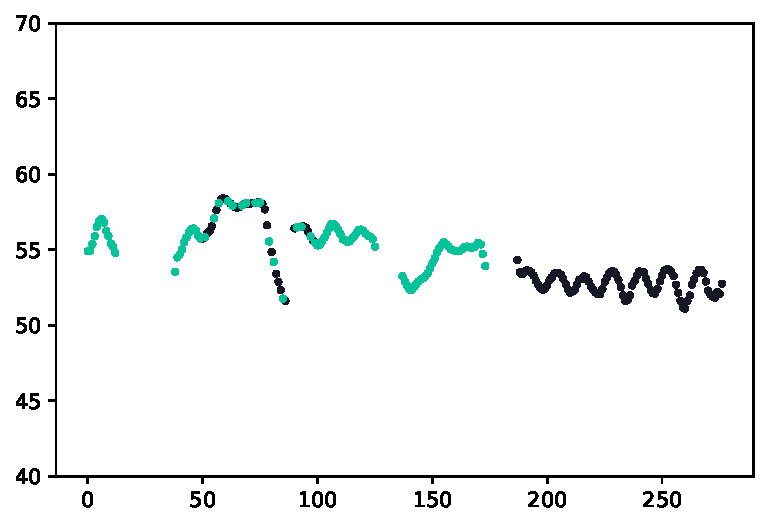
\includegraphics[scale=0.5]{../img/chyba_VR}
\caption{Příklady chyb špatné detekce melodie negativně ovlivňující metriku VR.}
\label{obr:chyba_VR}
\end{figure}

\subsubsection{Voicing Recall rate (Úplnost detekce)}

Poměr počtu časových oken, které byly správně označené jakožto obsahující melodii, a počtu časových oken doopravdy obsahujících melodii podle anotace.

    $$\mathrm{VR}(\mathbf{v}, \mathbf{v^*}) = \frac{\sum_\tau{v_\tau v^*_\tau}}{\sum_\tau{v^*_\tau}}$$

\begin{figure}[h!]\centering
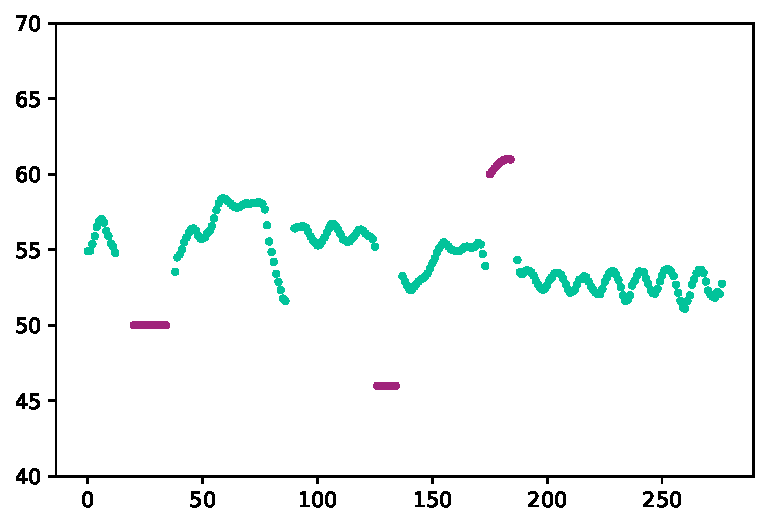
\includegraphics[scale=0.5]{../img/chyba_VFA}
\caption{Příklady chyb špatné detekce melodie zvyšující metriku VFA.}
\label{obr:chyba_VFA}
\end{figure}

\subsubsection{Voicing False Alarm rate (Nesprávné detekce)}

Poměr počtu časových oken, které byly nesprávně označené jako obsahující melodii, a počtu časových oken, které doopravdy melodii neobsahují. Pro interpretaci této metriky platí, že nižší hodnota je lepší, vyšší hodnota je horší.

    $$\mathrm{FA}(\mathbf{v}, \mathbf{v^*}) = \frac{\sum_\tau{v_\tau \bar{v}^*_\tau}}{\sum_\tau{\bar{v}^*_\tau}}$$


\begin{figure}[h!]\centering
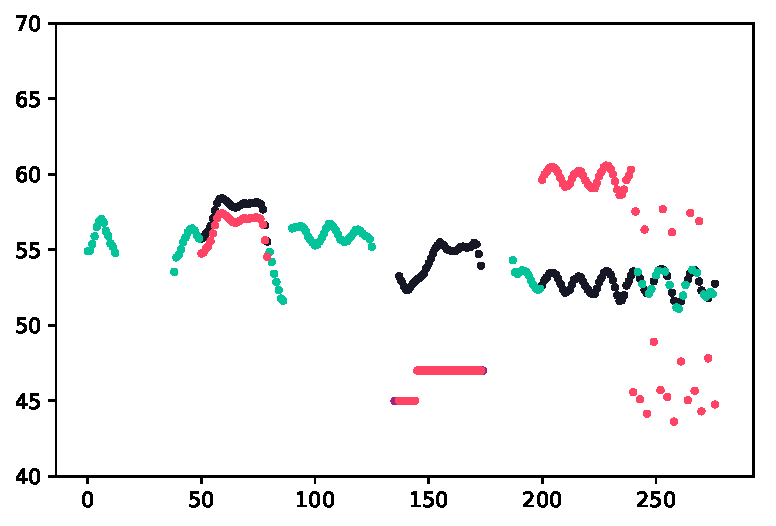
\includegraphics[scale=0.5]{../img/chyba_RPA}
\caption{Příklady chyb ovlivňujících metriku RPA a RCA.}
\label{obr:chyba_RPA}
\end{figure}


\subsubsection{Raw Pitch Accuracy (Přesnost odhadu výšky)}

Poměr správně odhadnutých tónů k celkovému počtu oken, které obsahují melodii. Výška správně určeného tónu se může lišit až o jeden půltón.


    $$\mathrm{RPA}(\mathbf{f}, \mathbf{f^*}) = \frac{\sum_\tau{v^*_\tau v_\tau \mathcal{T}[\mathcal{M}(f_\tau) - \mathcal{M}(f^*_\tau)}] }{\sum_\tau{v^*_\tau}}$$

kde $\mathcal{T}$ je prahová funkce

    \begin{equation*}
        \mathcal{T}[a] = \begin{cases}
                1 & \mathrm{pro} \abs{a} \le 0.5 \\
                0 & \text{jinak}
                
            \end{cases}
    \end{equation*}

Dodáme, že práh $0.5$ je v některých případech použití vhodné snížit na restriktivnější hodnoty, jako je $0.25$ nebo dokonce $0.1$. Jedná se zejména o použití metriky pro úlohu odhadu výšky jednohlasu (jako například v práci \cite{Kim2018}).

a $\mathcal{M}$ je funkce zobrazující frekvenci $f$ na reálné číslo počtu půltónů od nějakého referenčního tónu $f_{\mathrm{ref}}$ (například od 440 Hz, tedy komorního A4).

    $$\mathcal{M}(f) = 12 \log_2(\frac{f}{f_{\mathrm{ref}}})$$


\begin{figure}[h!]\centering
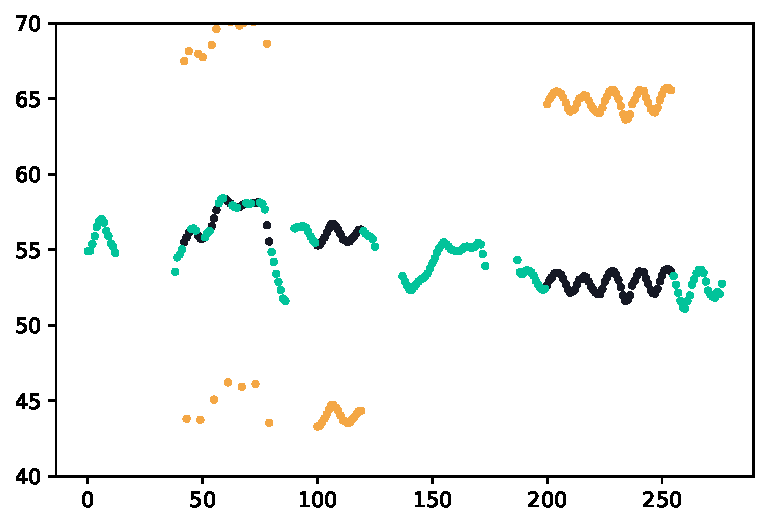
\includegraphics[scale=0.5]{../img/chyba_RCA}
\caption{Příklady chyb \uv{o oktávu} ovlivňujících pouze metriku RPA, nikoli metriku RCA.}
\label{obr:chyba_RPA}
\end{figure}

\subsubsection{Raw Chroma Accuracy (Přesnost odhadu výšky nezávisle na oktávě)}

Počítá se podobně jako \textit{Přesnost odhadu tónu}, výstupní a cílové tóny jsou však mapovány na společnou oktávu. Metrika tedy ignoruje chyby odhadu způsobené špatným určením oktávy tónu.

    $$\mathrm{RCA}(\mathbf{f}, \mathbf{f^*}) = \frac{\sum_\tau{v^*_\tau v_\tau \mathcal{T}[\langle \mathcal{M}(f_\tau) - \mathcal{M}(f^*_\tau)} \rangle_{12}] }{\sum_\tau{v^*_\tau}}$$

Nezávislost na oktávě zajistíme pomocí zobrazení rozdílu cílového a výstupního tónu na společnou oktávu.

    $$\langle a \rangle_{12} = a - 12 \lfloor \frac{a}{12} + 0.5 \rfloor  $$


\subsubsection{Overall Accuracy (Celková přesnost)}

Celková přesnost měří výkon algoritmu jak v odhadu melodie tak v detekci melodie. Počítá se jako podíl správně odhadnutých oken a celkového počtu oken.

    $$\mathrm{OA}(\mathbf{f}, \mathbf{f^*}) = \frac{\sum_\tau{v^*_\tau v_\tau \mathcal{T}[\mathcal{M}(f_\tau) - \mathcal{M}(f^*_\tau)}] + \bar{v}^*_\tau \bar{v}_\tau }{L}$$

\subsubsection{Poznámka k definicím metrik}

Definice RPA, RCA a OA zde uvedené se mírně liší od výchozích v práci \cite{Salamon2014}, jejich přímá implementace podle vzorce totiž vede kvůli nedostatečně dobře zadefinovanému vektoru frekvencí $\mathbf{f}$ k chybě, která se týká zejména metriky RCA. Ta v původním znění definice chybně zahrnovala jako správné tóny ty, které algoritmus odhadl jako nulové (tedy neznějící) a zároveň jejich pravdivá hodnota byla po zobrazení na jednu společnou oktávu blízká nule (tedy původní tón byl blízký nějakému násobku referenční frekvence). Kvůli zobrazení na společnou oktávu se stanou \uv{neznělé nulové odhady} a tóny blízké referenčním frekvencím nerozlišitelné a byly nesprávně považované za korektní. \footnote{
    Tato chyba byla přítomná i v nejpoužívanější, veřejné implementaci MIR metrik \textit{mir\_eval}. V praxi rozdíl chybné a opravené hodnoty této metriky na datasetu MedleyDB mohla dosahovat až sedmi procentních bodů, na repozitáři hostovaném na serveru Github jsme již spolu s autory chybu odstranili (odkaz na Github issue: \url{https://github.com/craffel/mir_eval/issues/311}). Opravný patch bude zahrnut do další verze balíku. Výsledky v této práci jsou počítány s opravenou verzí.}

\subsection{Další metriky}

Protože princip vnitřního fungování neuronových sítí často není zřejmý, je užitečné mít co nejvíce různých indikátorů, abychom měli při porovnávání jednotlivých modelů alespoň podrobnou informaci, v jakých ohledech se síť zlepšuje nebo zhoršuje. Pro tento účel jsem při práci implementoval další metriky, které při hledání architektur sítí pomáhaly.

\subsubsection{Chroma Overall Accuracy}

Počítá se obdobně jako Overall Accuracy, ale tóny jsou mapovány na společnou oktávu.

\subsubsection{Raw Harmonic Accuracy}

Metrika počítá odhadovaný tón jako správný, pokud se trefil do některé z harmonických frekvencí tónu. Protože je harmonických frekvencí teoreticky nekonečné množství, parametrem metriky je do jakého celočíselného násobku se ještě odhad počítá.

    $$\mathrm{RHA}(\mathbf{f}, \mathbf{f^*}, n) = \frac{\sum_{k=1}^n \sum_\tau{v^*_\tau v_\tau \mathcal{T}[\mathcal{M}(f_\tau) - \mathcal{M}(k f^*_\tau)} ] }{\sum_\tau{v^*_\tau}}$$

\subsubsection{Matice záměn not}

Pro podrobnější souhrnný přehled četností chyb se pro klasifikační úlohy používá matice záměn. Sloupce označují správné noty, řádky odhadované. Buňka na pozici $(x,y)$ má pak hodnotu podle četnosti odhadu noty $y$ místo správné noty $x$.

\subsubsection{Histogram vzdáleností odhadu}

Histogram hodnot rozdílu $\mathcal{M}(\mathbf{f}) - \mathcal{M}(\mathbf{f^*})$, tedy histogram vzdáleností odhadů výšky tónů od správné hodnoty.


\subsubsection{Kvalitativní příklady}

Modely byly při práci vyhodnocovány na několikaminutových množinách výňatků z validačních a testovacích dat. Metodika výběru spočívala v poslechu nahrávek a ručním výběru zajímavých hudebních jevů. Několik ukázek bylo také vybráno na základě seřazení nahrávek podle úspěšnosti přepisu stávajícími metodami a výběrem výňatků z tohoto seznamu nejproblematičtějších příkladů.



% - confusion matrix
% - estimation distance histogram
% - pitch accuracy per note

% \subsection{Limitace základních metrik}
% - limitace jsou předvedeny v onsets+frames
%     - nakonec nejsou, tam kritizují jenom 
% - například je otázka, jestli jsou všechny framy stejně důležité - zejména u vybrnkávání, piana, perkusí je otázka, kdy ještě anotovat, tedy jsou tam sporné konce. Na small_valid je to hodně vidět na té harfě
% - nijak se nepenalizuje nekontinualita výstupů, je rozdíl mezi 50\% accuracy, kde je zbytek unvoiced a 50\% accuracy, kde odhady strašně skáčou

% - Bosch metrics \cite{Bosch2016}
%     - Weighted Raw Chroma accuracy - počítá vzdálenost v oktávách
%     - Octave Jumps - vyjadřuje skokovitost o oktávy v po sobě následujících framech v rámci správných chroma odhadů
%     - Chroma continuity - 

% \section{Kvalitativní}

% - popsat můj small_validation

% - ilustrační příklady !!!
% 	- orchestrální i neorchestrální
% 		- metody z related work fungují na neorch.
% 	- jeden hlas
% 	- melodie nahoře (zkusit vybrat extrém ~ np.max(annotations))
% 	- melodie dole
% 	- melodie uprostřed

% 	- vlastnosti melodie
% 		- stabilní dlouhý tóny (a kolem doprovod)
% 		- něco proměnlivého
% 	- potichu/nahlas

\chapter{Experimenty}

V této kapitole prezentujeme přehled výsledků různých architektur pro extrakci melodie, trénované nad datasetem MedleyDB. Data byla rozdělena na trénovací, validační a testovací množinu tak, aby skladby od jednoho interpreta náležely právě do jedné z množin. Využili jsme existujícího rozdělení používaného v článcích \cite{Bittner2017} a \cite{DBasaranSEssid2018}, validační i testovací výsledky jsou tedy díky tomu porovnatelné s výsledky uvedenými v článcích.

Pro odhad výšky tónů porovnáváme architektury inspirované pracemi \cite{Kim2018}, \cite{Oord2016} a \cite{Bittner2017}. V prvním případě jde o architekturu CREPE původně navrženou pro sledování výšky tónů v jednohlasých nahrávkách. \cite{Oord2016} používají WaveNet složený z dilatovaných konvolucí pro generování lidské řeči. \cite{Bittner2017} používá hlubokou konvoluční síť pro kompletní přepis nahrávek i pro přepis melodie. 

Pro detekci melodie pak srovnáváme jednoduchou metodu práhování a složitější samostatný modul, založený na hlubokých neuronových sítích.

\section{Architektura CREPE}\label{sec:crepe}

První sada experimentů se zakládá na architektuře popsané v článku od \cite{Kim2018} použité pro sledování jednohlasu. Jak blíže popisujeme v kapitole \nameref{cha:souvisejici}, cílem monopitch trackingu je určit konturu základní frekvence melodického nástroje v jednohlasé nahrávce. Tato nahrávka se zpravidla skládá ze směsi čistého signálu hlasu a šumu v pozadí. Pokud však rozšíříme pojem šumu v pozadí tak, aby zahrnoval i melodický doprovod, pak dostáváme polyfonní signál, tedy vstupní signál pro metody extrakce melodie.

Jinými slovy je sledování jednohlasu speciálním případem extrakce melodie a tudíž přinejmenším stojí za zkoušku pokusit se tuto architekturu pro extrakci využít. Mimo to jednohlasé stopy často obsahují přeslech ostatních nástrojů, pokud nahrávka vznikala při společném hraní ve studiu, tudíž by model trénovaný na vícehlasé mixech mohl být robustní vůči tomuto druhu rušení. 

\begin{figure}[h]\centering
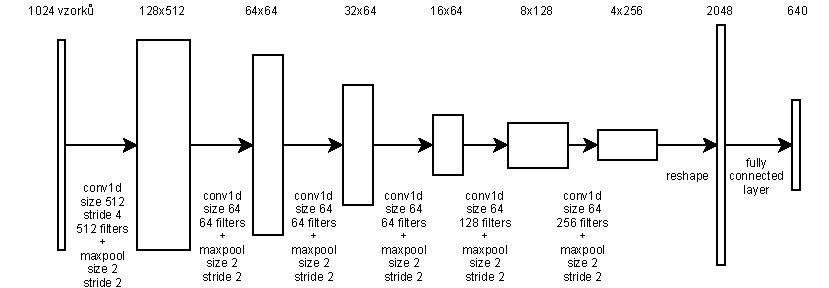
\includegraphics{../img/crepe_arch}
\caption{Diagram architektury CREPE, multiplikační koeficient 16x.}
\label{obr:wavenet_dilated}
\end{figure}

Architektura CREPE se skládá ze šesti konvolučních a pooling vrstev, pro regularizaci používá batch normalization a dropout po každé konvoluční vrstvě, jako nelineární aktivace je použita funkce ReLU. Po konvolucích následuje výstupní plně propojená vrstva, jako finální aktivační funkce je použita sigmoida. Vstupem modelu je okno o velikosti 1024 vzorků jednokanálového audio signálu, převzorkovaného na 16 kHz. Před první konvolucí je signál normalizován tak, aby každé jednotlivé vstupní okno mělo střední hodnotu 0 a směrodatnou odchylku 1. Podrobnější popis modelu je naznačen na obrázku.

Výsledný vektor o 640 složkách aproximuje pravděpodobnostní rozdělení výšky základní frekvence uprostřed vstupního okna, přičemž tento vektor pokrývá rozsah od noty $C_{-1}$ po $G_{9}$, mezi dvěma sousedními predikovanými tóny je vzdálenost 20 centů. Výšky tónů v centech označíme $\cent_1, \cent_2, \dots, \cent_{640}$. Rozsah tedy bezpečně pokrývá obvyklé hudební nástroje a na jednu notu připadá 5 složek (tónů) výsledného vektoru.

    $$\cent(f) = 1200 \log_2{\frac{f}{f_{\mathrm{ref}}}}$$

Pro trénování modelu potřebujeme také cílové diskrétní pravděpodobnostní rozdělení základní frekvence tónu. Jako cílovou pravděpodobnostní funkci použijeme normální rozdělení se střední hodnotou v bodě cílové základní frekvence $\cent(f_{\mathrm{ref}})$ a se směrodatnou odchylkou 25 centů. Toto rozdělení diskretizujeme tak, aby měl cílový vektor stejné dimenze jako odhadovaný.

    $$y_i = \frac{1}{\sqrt{2 \pi \sigma^2}}\exp{(-\frac{(\cent_i - \cent_{\mathrm{ref}})^2}{2 \sigma^2})}$$

Převod z pravděpodobnostní reprezentace výstupního vektoru na konkrétní hodnotu výšky noty provedeme pomocí výpočtu střední hodnoty výstupní distribuce. Jelikož by při výpočtu střední hodnoty ale hodnotu výsledné výšky tónu ovlivňoval i doprovod, který se na výstupním vektoru objevuje, počítáme střední hodnotu pouze z okolí maxima výstupu. Tím zajistíme, že získáme střední hodnotu gaussiánu náležícímu pouze jednomu tónu.

    $$ \left. \hat{\cent} = \sum_{\scaleto{i, \lvert \cent_i - \cent_m \rvert < 50}{8pt}} {\hat{y}_i \cent_i} \middle/ \sum_{\scaleto{i, \lvert \cent_i - \cent_m \rvert < 50}{8pt}} \hat{y}_i \right., m = \mathrm{argmax}_i(\hat{y}_i)$$

Optimalizovaná ztrátová funkce modelu (loss funkce) $\mathcal{L}(\mathbf{y}, \mathbf{\hat{y}})$ se počítá jako vzájemná korelace mezi vektorem cílových pravděpodobností $y$ a výstupním vektorem $\hat{y}$.

    $$\mathcal{L}(\mathbf{y}, \mathbf{\hat{y}}) = \sum_{i = 1}^{640}{(-y_i\log\hat{y}_i - (1-y_i)\log(1-\hat{y_i}))}$$

Optimalizace probíhá pomocí algoritmu Adam \citep{Kingma2014} s parametrem learning rate $0.0002$.

\begin{table}[h!]

\centering
    \begin{tabular}{l@{\hspace{1.5cm}}rrrrrrr}
    \toprule
    {}         &  \textbf{1.}   &  \textbf{2.}  &  \textbf{3.}  &  \textbf{4.}  &  \textbf{5.}   &  \textbf{6.}  &  \textbf{Celk. parametrů} \\
    \midrule
    CREPE 4x   &  128  &  16  &  16  &  16  &  32   &  64  &  $558\,240$ \\
    CREPE 8x   &  256  &  32  &  32  &  32  &  64   &  128 &  $177\,1200$ \\
    CREPE 16x  &  512  &  64  &  64  &  64  &  128  &  256 &  $6\,163\,200$ \\
    \bottomrule
    \end{tabular}

\caption{Počty filtrů v konvolučních vrstvách v architektuře CREPE v závislosti na multiplikačním koeficientu.}\label{tab:crepe_dimensions}

\end{table}

% rozepsat:
% - obhajoba raw signálu

% diskuze:
% - převzorkování na 16kHz
% - normalizace vstupu
% - formulace jako klasifikační úloha, nikoli regresní
% - je lepší odhadovat opravdové pravděpodobnostní rozdělení a nebo jejich škálované? (přijde mi, že kvůli sigmoid aktivaci bude jednodušší 1.0 = Truth, protože ty vstupní logity do sigmoid aktivace můžou být crazyshit velký)
% - crepe model - např. nedává vůbec smysl velikost kernelu 64 v posledních vrstvách, zbytečně se tam přidávají nuly jako padding
% - ukázat vizualizaci první vrstvy

\subsection{Replikace výsledků CREPE}

Abychom ověřili správnost implementace architektury CREPE pro sledování jednohlasu, spustíme model na syntetických, jednohlasých datech MDB-stem-synth, která byla zvěřejněná spolu s článkem od \cite{Salamon2017}.

Na rozdíl od článku \cite{Kim2018}, ve kterém autoři používají pro celkové vyhodnocení architektury pětinásobnou křížovou validaci, jsme použili pouze jednu trénovací a testovací množinu. Zásadní rozdíly mezi implementacemi modelu jsme na základě článku a veřejně dostupného kódu neobjevili.

Po jedné epoše trénování model dosáhl na testovací množině $98.6\%$ přesnosti odhadu výšky. \cite{Kim2018} uvádí přesnost modelu $97\%$. V jejich případě jde o průměrný výsledek pěti nezávislých běhů trénování a testování na různě rozdělených datových množinách. Rozdíl mezi dosaženými přesnostmi přičítáme odlišné evaluační strategii.

\begin{table}[h!]

\centering
    \begin{tabular}{llrr}
    \toprule
    Metrika & Práh & Průměrná hodnota & Hodnota \cite{Kim2018} \\
    \midrule
    RCA & 50 centů & 0.988 & 0.970 \\
    RPA  & 50 centů & 0.986 & 0.967 \\
    RPA  & 25 centů & 0.975 & 0.953 \\
    RPA  & 10 centů & 0.937 & 0.909 \\
    \bottomrule
    \end{tabular}
\caption{Výsledky pokusu o replikaci. Přesnosti nejsou přímo srovnatelné kvůli různým evaluačním strategiím.}\label{tab:crepe_dimensions}

\end{table}

Při replikaci experimentu jsme narazili na důležitost správného promíchání dat. Framework Tensorflow použitý pro trénování promíchává data vždy pomocí bufferu pevné velikosti pro dvojice vstupů a cílových výstupů. V praxi je však potřeba buď nastavit buffer na velikost větší než je celková velikost datasetu, a nebo implementovat vlastní míchání přes všechna dostupná data. Při nedostatečně promíchaných datech totiž trénovací dávka (batch) není reprezentativní pro celý dataset, ale pouze pro jeho podmnožinu, což se negativně projevuje kolísající validační přesností modelu.

\subsection{CREPE pro extrakci melodie}

Jako první experiment extrakce melodie z polyfonních dat spustíme nezměněnou architekturu CREPE, v následujících experimentech se tuto baseline pokusíme překonat. Abychom urychlili trénování následujících experimentů, přesnost určíme pro sítě s různou kapacitou. Pokud se výsledky při různých kapacitách nebudou příliš lišit, můžeme experimenty provádět s architekturou s nižší kapacitou a tím snížit trénovací čas. Kapacity upravíme pomocí multiplikačního koeficientu počtu filtrů u všech konvolučních vrstev, počty filtrů jsou uvedeny v tabulce \ref{tab:crepe_dimensions}.

% TODO: diskuse o under a overfittingu

\begin{table}[h!]

\centering
    % \begin{tabular}{l@{\hspace{1.5cm}}rr}
    % \toprule
    % \textbf{Model}      &  \textbf{RPA}    &  \textbf{RCA} \\
    % \midrule
    % CREPE 4x   &  0.634  &  0.753 \\
    % CREPE 8x   &  0.661  &  0.766 \\
    % CREPE 16x  &  0.666  &  0.771 \\
    % \bottomrule
    % \end{tabular}
% \begin{tabular}{lrrr}
% \toprule
% {} &  Raw Pitch Accuracy &  Raw Chroma Accuracy &  Voicing Accuracy \\
% \thead{Multiplikátor \\ kapacity sítě} &                     &                      &                   \\
% \midrule
% \textbf{4                          } &               0.634 &                0.753 &             0.534 \\
% \textbf{8                          } &               0.661 &                0.766 &             0.534 \\
% \textbf{16                         } &               0.666 &                0.771 &             0.534 \\
% \textbf{32                         } &               0.656 &                0.753 &             0.591 \\
% \bottomrule
% \end{tabular}

\begin{tabular}{rrr}
\toprule
Mult. koef. kapacity &   RPA &   RCA \\
\midrule
                   4 & 0.634 & 0.753 \\
                   8 & 0.661 & 0.766 \\
                  16 & 0.666 & 0.771 \\
                  32 & 0.656 & 0.753 \\
\bottomrule
\end{tabular}
\caption{Výsledky experimentu s různými kapacitami modelu.}\label{tab:crepe_capacity}
\end{table}

\begin{figure}[h]\centering
    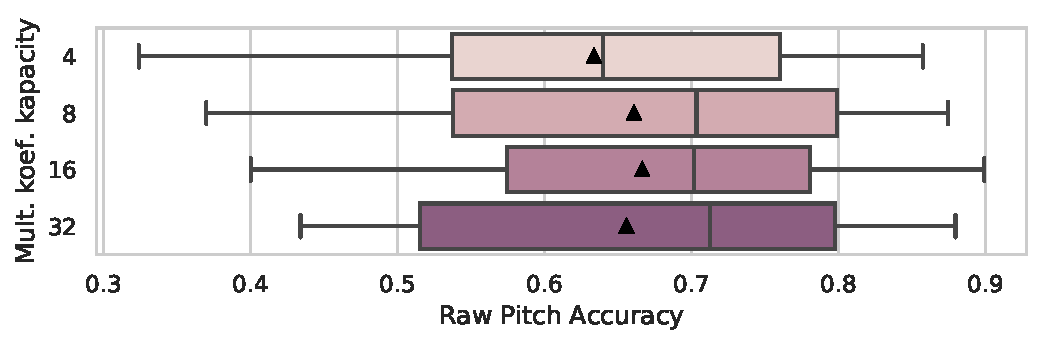
\includegraphics[scale=0.6]{../img/figures/crepe_kapacita.pdf}
\caption{Výsledky experimentu s různými kapacitami modelu.}
\label{obr:crepe_capacity}
\end{figure}

Z validačních výsledků po $200\,000$ iteracích (přibližně 6 epoch) vidíme, že se výsledek modelů CREPE 8x a CREPE 16x liší řádově o desetiny procentních bodů. Přitom model s větší kapacitou se trénuje o 35\% delší dobu. Proto pro další srovnávání zvolíme architektury s multiplikačním koeficientem 8, modely s dobrými výsledky případně přetrénujeme s vyšší kapacitou.

\subsection{Vliv rozlišení diskretizace výšky noty}

Otestujeme nastavení granularity výstupního vektoru. V článku \cite{Kim2018} se totiž důvod volby pěti frekvencí na notu nediskutuje. Intuitivně by však mělo vyšší rozlišení spíše pomáhat, důvodem je, že nástroje a zejména lidský hlas se často při hraní odchylují od přesných, definovaných frekvencí hraných not a vyšší rozlišení tyto odchylky může lépe zachytit. Ve výsledku by pak síť s jemnějším výstupem měla dělat méně chyb, kde se skutečná a výstupní hodnota liší o jeden půltón.


\begin{table}[h!]

\centering
    \begin{tabular}{rrr}
    \toprule
    Jemnost diskretizace &   RPA &   RCA \\
    \midrule
                    1 & 0.612 & 0.711 \\
                    3 & 0.653 & 0.760 \\
                    5 & 0.666 & 0.771 \\
                    7 & 0.654 & 0.763 \\
                    9 & 0.658 & 0.760 \\
    \bottomrule
    \end{tabular}

\caption{Architektura CREPE s různou jemností diskretizace.}\label{tab:crepe_diskretizace}

\end{table}

\begin{figure}[h]\centering
    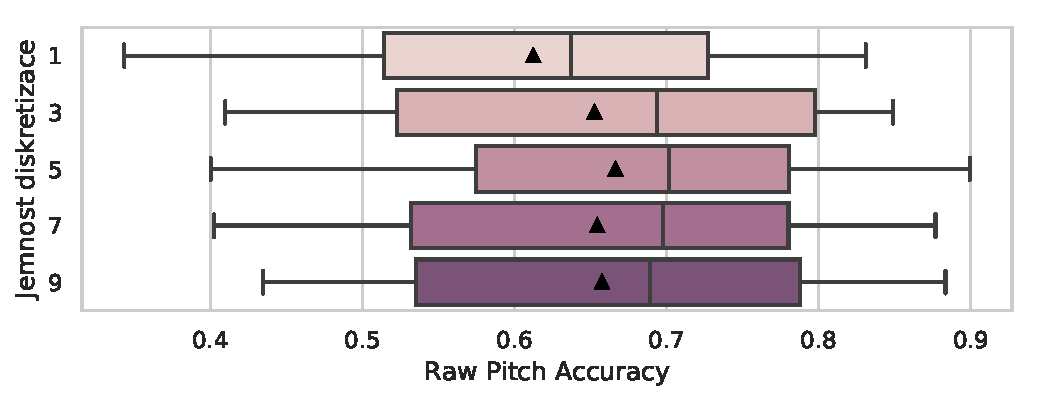
\includegraphics[scale=0.6]{../img/figures/crepe_diskretizace.pdf}
\caption{Architektura CREPE s různou jemností diskretizace.}\label{obr:crepe_diskretizace}
\end{figure}

Jak můžeme pozorovat na výsledných hodnotách, jemná granularita výstupu jednoznačně zlepšuje přesnost sítě. Abychom ověřili domněnku, že vyšší rozlišení pomáhá zmenšit počet chyb o půltón, vytvoříme histogram vzdáleností cílového a odhadovaného tónu. V tomto histogramu by pak měl být zřetelný pokles v příslušných třídách. Podle histogramu se počet chyb o půltón mezi zkoumanými modely liší téměř o polovinu, zlepšení tohoto druhu chyb je tedy podstatné.

\begin{figure}[h]\centering
    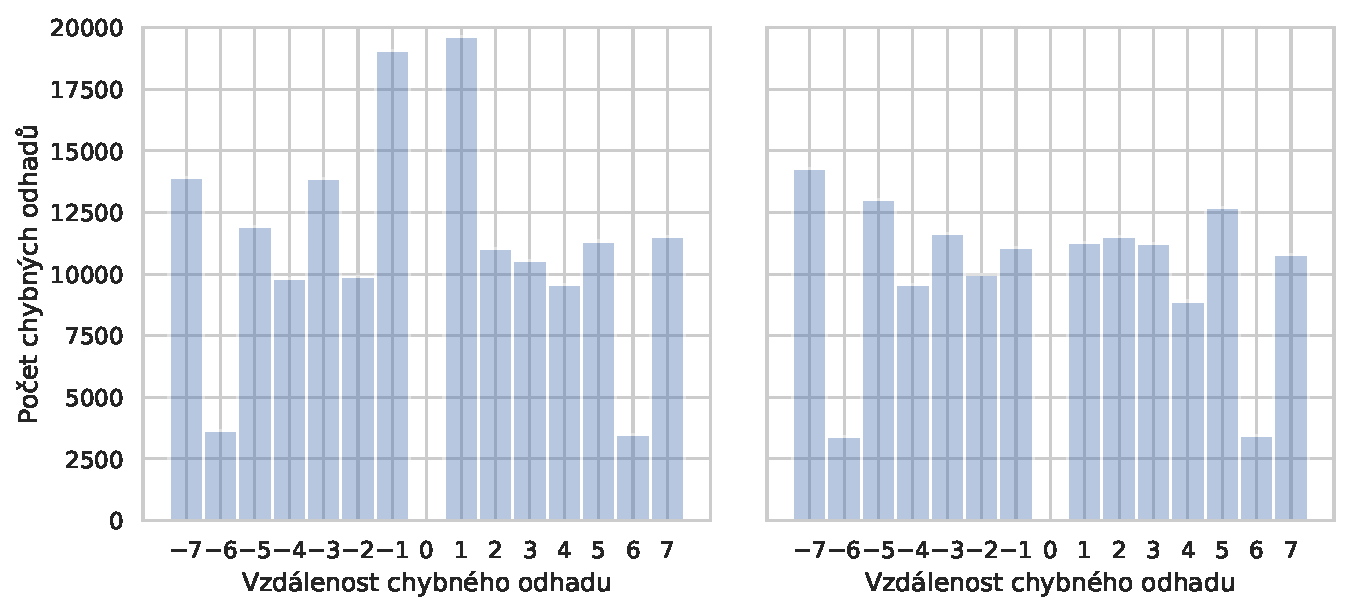
\includegraphics[scale=0.6]{../img/figures/crepe_diskretizace_hist.pdf}
\caption{Histogramy vzdálenosti chybného odhadu, výstup prvního modelu má rozlišení 50 centů, výstup druhého 10 centů.}\label{obr:crepe_diskretizace}
\end{figure}

\textcolor{red}{odsud dolů přepsat}

\subsection{Vliv rozptylu cílové pravděpodobnostní distribuce výšky noty}

Podle \cite{Bittner2017} pomáhá cílová distribuce s vyšším rozptylem snížit penalizaci sítě za téměř korektní odhady výšek tónů. Mimo to u dostupných dat často nejsou anotace naprosto perfektní, jisté rozostření hranice anotace tudíž pomáhá i v případě nepřesné cílové anotace, síť pak není tolik penalizována za svou případnou správnou odpověď. 

V článku se však nediskutuje, proč bylo zvoleno nastavení směrodatné odchylky na 20 centů. \cite{Kim2018} používá odchylku 25 centů a není na první pohled zřejmé, jaká je optimální hodnota. Příliš vysoký rozptyl způsobí, že síť bude tolerovat více chyb o půltón, příliš nízký rozptyl naopak penalizuje i téměř správné odhady. Intuitivně se nejlepší nastavení pravděpodobně bude pohybovat kolem používaných 25 centů, jelikož to je hranice chybné klasifikace, na druhou stranu optimální hodnota jistě bude závislá na nastavení rozlišení výstupního vektoru, jelikož nižší rozlišení bude jistě vyžadovat vyšší hodnotu rozptylu (v extrémním případě rozptylu blížícího se k nule a cílové frekvence mimo kvantizační hladiny by vzniklý cílový vektor nemusel obsahovat žádné ostré maximum).

Poznamenám také technický detail, který je důležitý při samotné implementaci. Přestože jsem cílový výstup sítě zadefinoval jako diskrétní pravděpodobnostní rozdělení, při trénování je tento vektor hodnot pronásoben koeficientem tak, aby $\max(\mathbf{y}) = 1.0$ a tedy součet prvků vektoru není roven jedné (a o pravděpodobnostní rozdělení se doopravdy nejedná). Důvodem je použití aktivační funkce *sigmoid* u výstupní vrstvy, která nezaručuje výstup korektního rozdělení. Díky tomu se na výstupu může objevit různé množství stejně pravděpodobných kandidátů na melodii.

Testovaná síť má vstupní okno široké 4096 vzorků, používá multiplikátor kapacity 16x a vstup zpracovává 6 různě širokými konvolučními vrstvami (viz experiment *Vliv násobného rozlišení první konvoluční vrstvy*).


\begin{table}[h!]
\centering
    \begin{tabular}{rrr}
    \toprule
    Rozptyl &   RPA &   RCA \\
    \midrule
    0.000 & 0.657 & 0.759 \\
    0.088 & 0.672 & 0.775 \\
    0.124 & 0.677 & 0.773 \\
    0.177 & 0.689 & 0.784 \\
    0.221 & 0.677 & 0.771 \\
    0.265 & 0.677 & 0.770 \\
    0.354 & 0.669 & 0.773 \\
    0.707 & 0.654 & 0.757 \\
    \bottomrule
    \end{tabular}

\caption{Architektura CREPE, vliv rozptylu cílové distribuce.}\label{tab:crepe_diskretizace}
\end{table}

\begin{figure}[h]\centering
    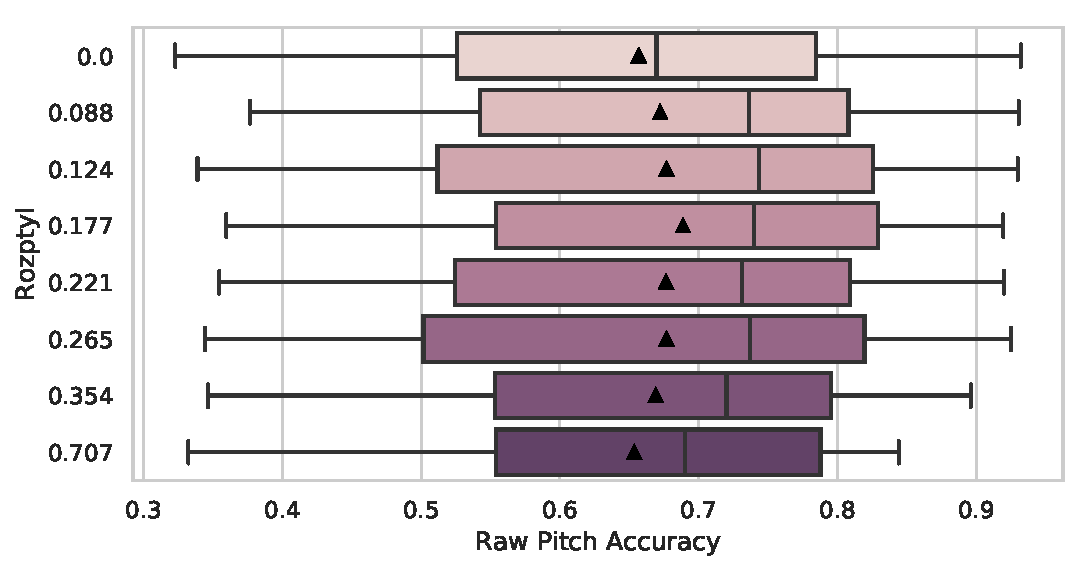
\includegraphics[scale=0.6]{../img/figures/crepe_rozptyl.pdf}
\caption{Architektura CREPE, vliv rozptylu cílové distribuce.}\label{obr:crepe_diskretizace}
\end{figure}



Z experimentů vyplývá, že optimální směrodatná odchylka se pohybuje kolem hodnoty $0.177$, tedy níže než v porovnávaných pracích. 

% ------
% - cílová distribuce doopravdy není distribuce
% - ty zvláštní testované směrod. odchylky jsou kvůli mé chybné implementaci rozostřování
% - zde můžu přidat obrázek, jak vypadají anotace
%     mám to rozpracované na: http://jirkabalhar.cz:6088/notebooks/bakalarka/algoritmy/ismir2017-deepsalience/deepsalience/out/io_comparison.ipynb#

\subsection{Vliv šířky vstupního okna}

Architektura CREPE byla navržena pro monopitch tracking, dá se předpokládat, že jelikož je v monofonních nahrávkách oproti polyfonním daleko méně (melodického) šumu, není pro určení výšky tónu potřeba větší kontext než použitých 1024 vzorků (při vzorkovací frekvenci 16kHz toto odpovídá 64 milisekundám audia). To ale nemusí platit pro složitější signály, kde by síť mohla z delšího kontextu těžit. Otestujeme tedy vliv většího vstupního okna na výslednou přesnost.


\begin{table}[h!]
\centering
    \begin{tabular}{rrr}
    \toprule
    Šířka vstupního okna &   RPA &   RCA \\
    \midrule
    512 (32 ms)   & 0.634 & 0.748 \\
    1024 (64 ms)  & 0.645 & 0.763 \\
    2048 (128 ms) & 0.648 & 0.760 \\
    4096 (256 ms) & 0.650 & 0.762 \\
    8192 (512 ms) & 0.675 & 0.775 \\
    \bottomrule
    \end{tabular}

\caption{Architektura CREPE, vliv šířky vstupního okna.}\label{tab:crepe_sirka}
\end{table}

\begin{figure}[h]\centering
    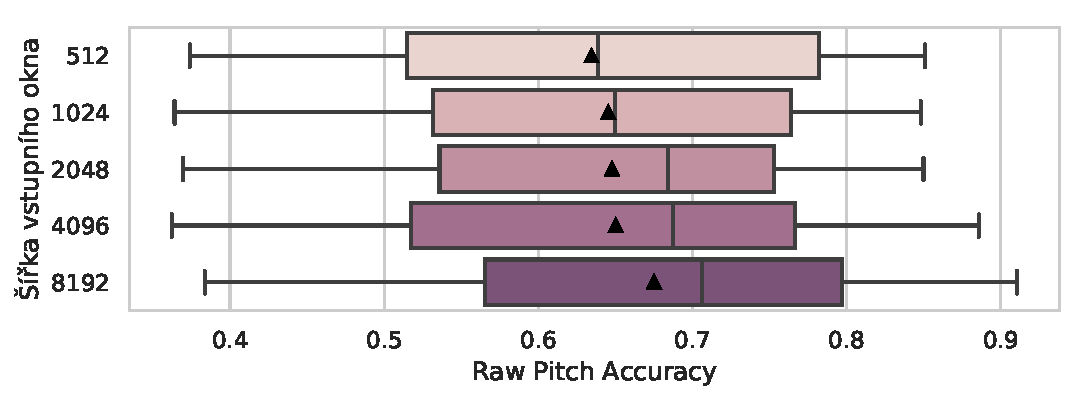
\includegraphics[scale=0.6]{../img/figures/crepe_sirka.pdf}
\caption{Architektura CREPE, vliv rozptylu cílové distribuce.}\label{obr:crepe_sirka}
\end{figure}

% TODO: možná by to chtělo taky přetrénovat

% - širší okno se také hodí pro onsety a offsety

\subsection{Vliv násobného rozlišení první konvoluční vrstvy}

Podle \cite{Kim2018} se přesnost CREPE snižuje s výškou tónu. Autoři si tuto skutečnost vysvětlují neschopností modelu generalizovat na barvy a výšky tónů neobsažených v trénovací množině, generalizaci by ale mohla pomoci také úprava modelu. Protože k rozpoznání vyšších frekvencí stačí méně vzorků než pro rozpoznání nižších, mohli bychom se pokusit upravit první konvoluční vrstvu sítě, která tento úkol zastává, a rozdělit ji na množiny různě širokých konvolucí, jejichž kanály následně sloučíme zpět do jednotné vrstvy. To by mělo mít za následek, že rozpoznávání vysokých tónů budou zastávat užší konvoluce a jejich kernel bude jednodušší než široké kernely s vysokou mírou redundance.

První vrstvu s kernelem s 256 filtry (tj. počet filtrů první vrstvy s multiplikátorem 8x, viz první experiment) jsem rozdělil na vícero různě širokých kernelů s menším počtem filtrů, tak aby kapacita sítě zůstala přibližně stejná a sítě byly porovnatelné. 

\begin{table}[h!]
\centering
    \begin{tabular}{lrrrrrrrrr}
    \toprule
    Šířka vrstev & 512 & 256 & 128 & 64 & 32 & 16 & 8  & 4  & Počet parametrů  \\
    Počet vrstev & {} & {} & {} & {} & {} & {} & {}  & {}  & {}  \\
    \midrule
    1                   & 256 &     &     &    &    &    &    &    & 2098880 \\
    2                   & 128 & 128 &     &    &    &    &    &    & 2066112 \\
    3                   & 85  & 85  & 85  &    &    &    &    &    & 2041918 \\
    4                   & 64  & 64  & 64  & 64 &    &    &    &    & 2029248 \\
    5                   & 51  & 51  & 51  & 51 & 51 &    &    &    & 2016350 \\
    6                   & 42  & 42  & 42  & 42 & 42 & 42 &    &    & 2001944 \\
    7                   & 36  & 36  & 36  & 36 & 36 & 36 & 36 &    & 1996184 \\
    8                   & 32  & 32  & 32  & 32 & 32 & 32 & 32 & 32 & 2000448 \\
    \bottomrule
    \end{tabular}
\caption{Počet filtrů prvních vrstev multirezoluční vstupní konvoluční vrstvy.}\label{tab:crepe_velikosti_multirozliseni}
\end{table}

Experiment jsem provedl na síti se vstupním oknem 2048 vzorků, multiplikátorem kapacity 8, 

\begin{table}[h!]
\centering
    \begin{tabular}{rrr}
    \toprule
    Počet konvolučních vrstev &   RPA &   RCA \\
    \midrule
                            1 & 0.669 & 0.779 \\
                            2 & 0.669 & 0.773 \\
                            3 & 0.672 & 0.773 \\
                            4 & 0.674 & 0.778 \\
                            5 & 0.686 & 0.781 \\
                            6 & 0.678 & 0.780 \\
                            7 & 0.677 & 0.779 \\
                            8 & 0.680 & 0.778 \\
    \bottomrule
    \end{tabular}
\caption{Architektura CREPE, vliv multirezoluční vstupní konvoluční vrstvy.}\label{tab:crepe_multirozliseni}
\end{table}

\begin{figure}[h]\centering
    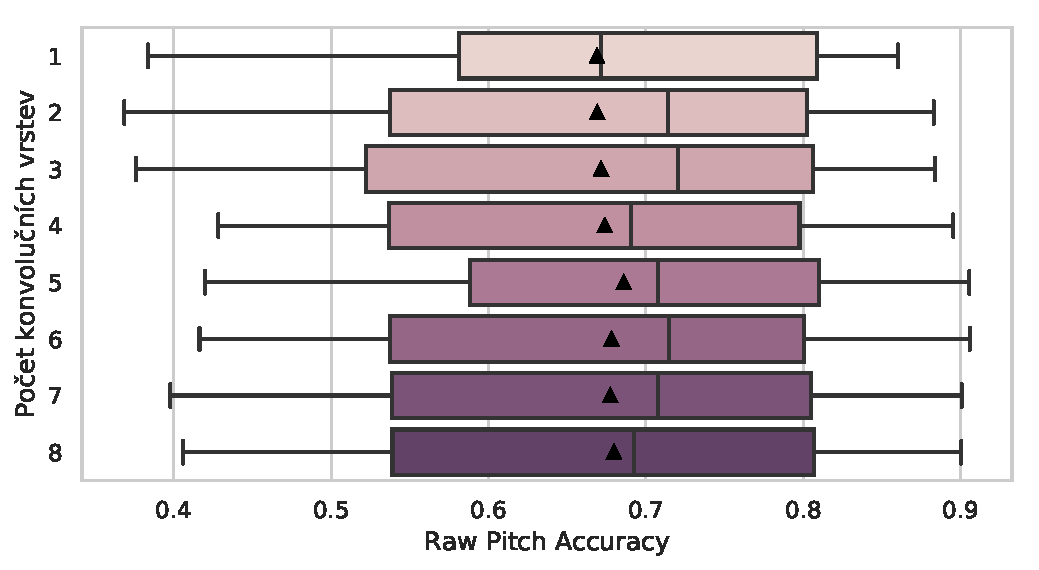
\includegraphics[scale=0.6]{../img/figures/crepe_multirozliseni.pdf}
\caption{Architektura CREPE, vliv multirezoluční vstupní konvoluční vrstvy.}\label{obr:crepe_multirozliseni}
\end{figure}

Zlepšení výsledků se pohybuje v řádu desetin procentních bodů, tedy není příliš vysoké. Zlepšení je nejvíce patrné v případě pěti různě širokých konvolučních vrstev, kde dosahuje $1.3$ procentního bodu. Analýzou výsledků přesnosti podle výšky noty se mi nepodařilo prokázat domněnku, že by konvoluce s více rozlišeními pomáhala u odhadu not vyšších frekvencí. Její přínos je drobný a projevuje se na většině frekvenčních pásem.


\section{Architektura WaveNet}

Generativní model WaveNet popsaný týmem \cite{Oord2016} je architektura navržená pro generování zvukového signálu. Autoři však v článku zmiňují, že se architekturu pokusili využít i pro převod mluvené řeči na text (dataset TIMIT), a podařilo se jim dosáhnout výsledků srovnatelných se state-of-the-art. Architektura spočívá ve vrstvení dilatovaných konvolucí s rozšiřujícím se rozsahem. Díky exponenciálně rostoucím dilatacím se také exponenciálně zvětšuje receptivní pole jednotlivých konvolučních vrstev. Díky této vlastnosti pak například stačí pro pokrytí 1024 vzorků vstupu pouze 9 vrstev s šířkou kernelu 2 a dilatacemi 1,2,4,8 ... 512. Pokud bychom stejného receptivního pole chtěli dosáhnout pomocí obvyklých konvolucí počet potřebných vrstev by byl lineární vzhledem k šířce pole. Vrstvení konvolucí je porovnáno na obrázcích \ref{obr:wavenet_conv} a \ref{obr:wavenet_dilated}. Síť tedy velmi snadno pokryje široký kontext, což je vlastnost, která je pro zpracování zvukového signálu užitečná.

\begin{figure}[h]\centering
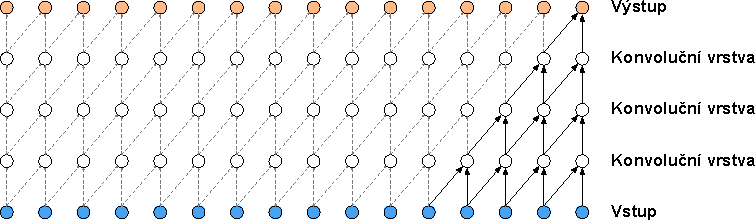
\includegraphics{../img/wavenet_konvoluce}
\caption{Vrstvení obyčejných konvolucí s lineárně rozšiřovaným dosahem, obrázek převzat z \cite{Oord2016}.}
\label{obr:wavenet_conv}
\end{figure}

\begin{figure}[h]\centering
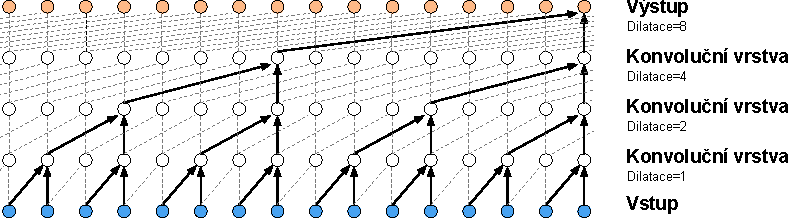
\includegraphics{../img/wavenet_dilatace_konvoluce}
\caption{Vrstvení dilatovaných konvolucí s exponenciálně rozšiřovaným dosahem, obrázek převzat z \cite{Oord2016}.}
\label{obr:wavenet_dilated}
\end{figure}

Síť se pro Music Information Retrieval úlohy od svého zveřejnění příliš neuchytila. Její použití se v oblasti hudby se omezuje na generativní úlohy (\cite{Hawthorne2018a}, \cite{Yang2017}, \cite{Engel2017} a další), případně pro source-separation \citep{Stoller2018}. Jediný publikovaný pokus s použitím architektury WaveNet pro příbuznou úlohu kompletního automatického přepisu podnikli \cite{Martak2018} s použitím datasetu MusicNet. Jejich model však netestovali na standardních evaluačních datasetech ze soutěže MIREX, tudíž není zřejmé, jakých výsledků v porovnání s existujícími metodami autoři dosáhli.



\begin{figure}[h]\centering
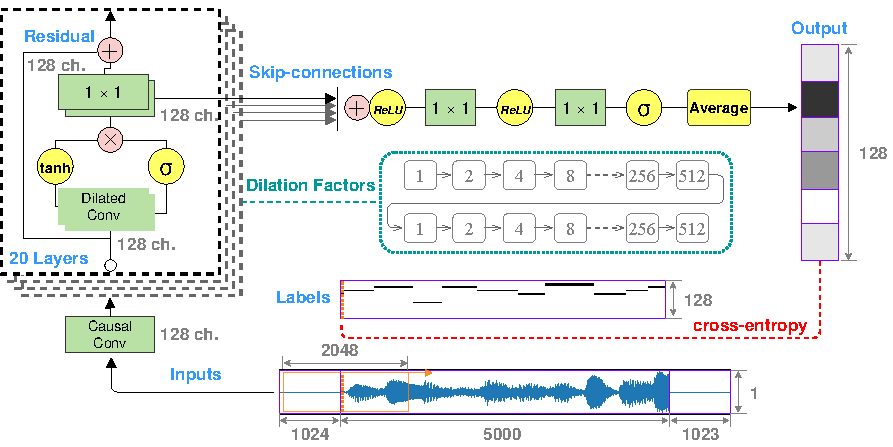
\includegraphics{../img/wavenet_arch}
\caption{Architektura WaveNet upravená pro kompletní přepis skladeb, upraveno na základě \cite{Martak2018}.}
\label{obr:wavenet_arch}
\end{figure}

\subsection{Baseline na základě \cite{Martak2018}}

% python -u wavenet.py --evaluate --filter_width 2 --initial_filter_width 2 --max_dilation 512 --stack_number 2 --residual_channels 128 --skip_channels 128 \
%     --batch_size 20 --min_note 0 --note_range 128 --bins_per_semitone 1 --annotation_smoothing 0 \
%     --iterations 100000 --learning_rate_decay_steps 10000 --learning_rate_decay 0.8 --annotations_per_window 5 --context_width 2100 --use_biases --frame_width 160 \
%     --skip add --postprocessing "conv_f128_k1_s1_Psame_arelu--conv_f128_k1_s1_Psame--avgpool_p160_s160_Psame"


Pro extrakci melodie využijeme jako výchozí model upravenou architekturu od \cite{Martak2018}, jejíž struktura je naznačena na obrázku \ref{obr:wavenet_arch}. Vstupem je okno velikosti 4894 vzorků audia převzorkovaného na $16\,\rm kHz$, toto okno nejprve zpracujeme standardní konvoluční vrstvou s šířkou kernelu 2 a 128 výstupními kanály, takto zpracovaný signál dále prochází dvěma bloky po desíti vrstvách, které obsahují dilatované konvoluce. Vrstvy obsahují dvě dilatované konvoluce, jednu s aktivací hyperbolickým tangens a jednu s aktivační funkcí sigmoid. Výstupy těchto konvolucí jsou po složkách vynásobeny, díky čemuž konvoluce s aktivací sigmoid funguje jako nastavitelná propust signálu (Gated activation unit, \cite{Oord2016a}), poté je výstup opět zpracován dvěmi konvolucemi, tentokrát se šířkou kernelu 1x1. Výstup první sečteme s původním vstupem celé vrstvy (jedná se o residuální propojení poprvé popsané v práci \cite{He2015}) a zpracujeme ho nadcházející vrstvou. Výstup druhé konvoluce (autoři tuto cestu nazývají \emph{skip propojení}) zařadíme mezi výstupy skip propojení všech ostatních vrstev.

Pro výpočet odhadů výšky tónu sečteme všechna skip propojení, tento součet zpracujeme dvěma konvolucemi, druhá z nich má na výstupu 128 kanálů zpracovaných sigmoidou, což odpovídá rozsahu odhadovaných not. Jelikož všechny popsané transformace zachovávají šířku vstupu, dostáváme po této konvoluci odhady výšek not pro každý vstupní vzorek zvuku, taková anotace je zbytečně podrobná, tudíž výsledné anotace podvzorkujeme pomocí pooling vrstvy počítající průměr hodnot.

\begin{figure}[h]\centering
    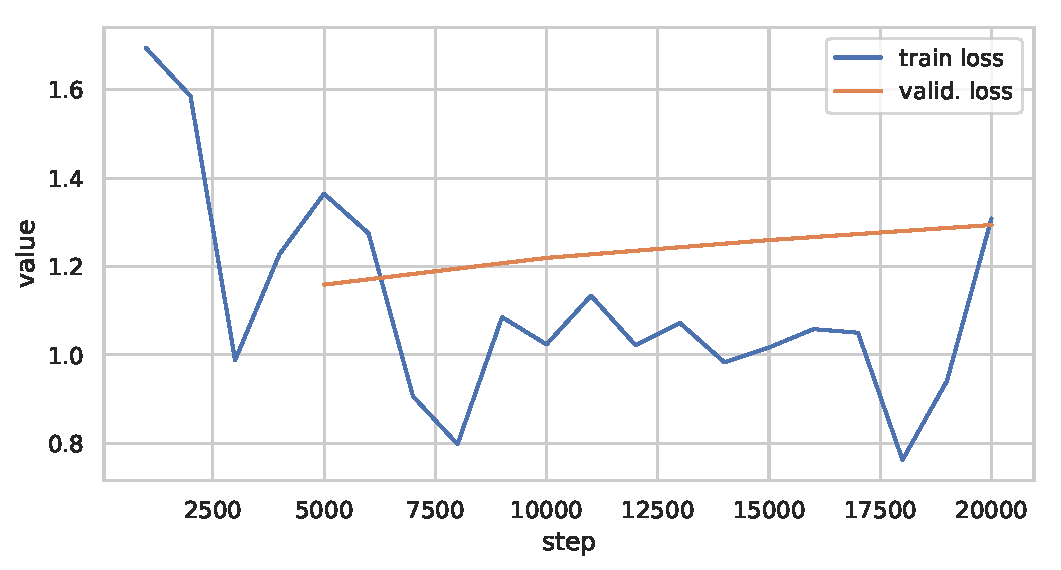
\includegraphics[scale=0.6]{../img/figures/wavenet_overfit}
    \caption{Vývoj ztrátové funkce při učení architektury \cite{Martak2018} pro extrakci melodie. Zatímco hodnoty pro trénovací množinu mají klesající tendenci, hodnoty na validační množině rostou, síť se velmi rychle přeučuje.}\label{obr:wavenet_overfit}
\end{figure}

Po $20\,000$ iteracích s velikostí dávky 20 a parametrem learning rate $0.001$ síť dosahuje na validačních datech přesnost odhadu tónu $0.583$ (RPA) a přesnost odhadu tónu nezávisle na oktávě $0.692$ (RCA). V porovnání s výsledky architektury CREPE jsou tyto výsledky výrazně nižší, krom toho učení sítě trvá velmi dlouho (14 minut na 1000 iterací), zejména kvůli obrovské kapacitě a topologické komplexitě modelu ($2\,009\,728$ trénovatelných parametrů). Veliká kapacita modelu také způsobuje přeučení sítě (viz \ref{obr:wavenet_overfit}), pokusíme se tedy zrychlit trénování a zabránit přeučení výrazným snížením počtu filtrů dilatačních a skip propojení ze 128 na 16, a použitím pouze jednoho dilatačního bloku. Také snížíme velikost trénovací dávky na 8 pro další zrychlení učení. Nová síť obsahuje 10 vrstev s dilatacemi $(1, 2, 4, 8, \dots, 512)$, a tedy $34\,736$ parametrů a dosahuje RPA $0.598$ a RCA $0.696$ po $100\,000$ iteracích při rychlosti trénování 30 sekund na 1000 iterací. Síť tedy dosahuje stejných výsledků ve výrazně kratším čase.

Z předchozích experimentů na architektuře CREPE víme, že jemnější výstupní reprezentace pomáhá snížit počet chyb o půltón, upravíme tedy síť tak, aby na jeden půltón připadalo 5 výstupních složek vektoru, zmenšíme výstupní frekvenční rozsah a hodnoty cílového vektoru změníme z ostré predikce konkrétního tónu na \uv{rozmlžený} gaussián se směrodatnou odchylkou $18\,\rm centů$ (pro podrobnější popis viz \ref{sec:crepe}). Síť po této úpravě dosahuje RPA 0.629 a RCA 0.731 po $100\,000$ iteracích. 

\begin{figure}[h]\centering
    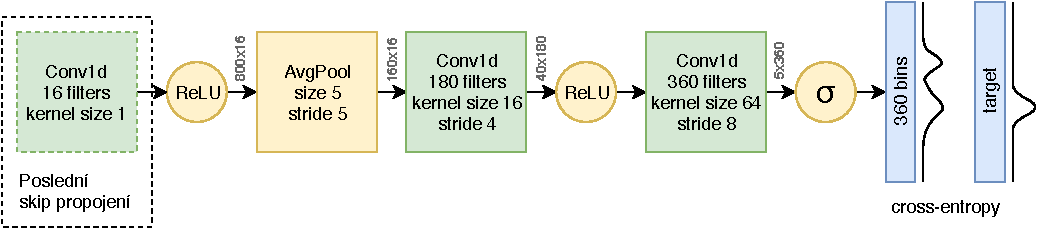
\includegraphics[scale=0.8]{../img/wavenet_lastlayer}
    \caption{Úprava posledních vrstev WaveNet architektury.}\label{obr:wavenet_lastlayer}
\end{figure}

Předběžným hledáním výchozí architektury pro nadcházející sadu experimentů jsme došli k následujícím úpravám. Dilatované konvoluce ve všech vrstvách mají šířku 3 místo 2, jejich vstup tedy závisí na všech okolních vzorcích, nikoli jen na předchozích, jak je naznačeno na obrázku \ref{obr:wavenet_dilated}. Dále jsme odstranili konvoluční vrstvu, která zpracovává vstup, ten je tedy přímo zpracován dilatačním blokem. Ze skip propojení se zpracovává pouze poslední, nedochází ke sčítání všech, což je úprava, kterou pro přepis řeči používají původní autoři článku WaveNet \cite{Oord2016}. Tento výstup je následně zpracován pooling vrstvou a dvěmi konvolucemi se skoky (stride), viz obrázek \ref{obr:wavenet_lastlayer}. Tato síť dosahuje RPA 0.655 a RCA 0.759 po $100\,000$ iteracích a je základem pro následující experimenty.

\subsection{Vliv počtu filtrů dilatačních vrstev a skip propojení}

Jedním ze zásadních faktorů ovlivňujících kapacitu sítě je počet filtrů dilatačních vrstev a skip propojení. Tyto kanály nesou informaci o vzorku a jeho okolí, v závislosti na vrstvě dilatace. Výstup poslední vrstvy má tedy délku počtu vstupních vzorků 2848 a 16 kanálů. Každý výstupní vzorek nese informaci o svém okolí délky 2047. Podobně jako v případě architektury CREPE nalezneme vhodnou kapacitu sítě tak, aby nedocházelo k přeučení (overfitting) ani k nedoučení (underfitting) na trénovací množině.

\begin{table}[h!]
\centering
    \begin{tabular}{rrr}
    \toprule
    Počet kanálů &   RPA &   RCA \\
    \midrule
            4 & 0.609 & 0.714 \\
            8 & 0.628 & 0.739 \\
            16 & 0.655 & 0.759 \\
            24 & 0.665 & 0.764 \\
            32 & 0.671 & 0.771 \\
            40 & 0.667 & 0.766 \\
            48 & 0.667 & 0.764 \\
    \bottomrule
    \end{tabular}

\caption{Architektura WaveNet, vliv počtu filtrů dilatačních vrstev a skip propojení.}\label{tab:wavenet_dil_skip_channels}
\end{table}

\begin{figure}[h]\centering
    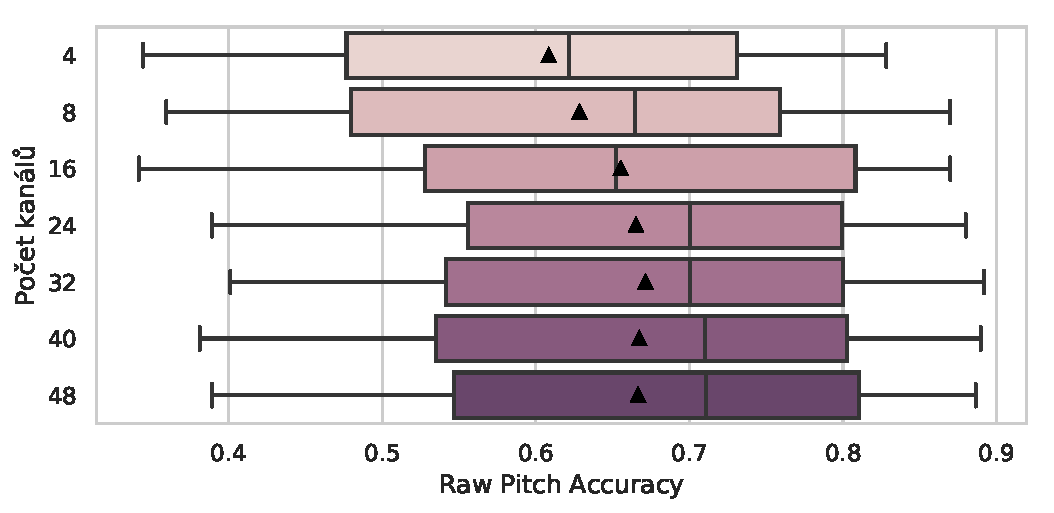
\includegraphics[scale=0.6]{../img/figures/wavenet_dil_skip_channels.pdf}
\caption{Architektura WaveNet, vliv počtu filtrů dilatačních vrstev a skip propojení.}\label{obr:wavenet_dil_skip_channels}
\end{figure}

Na základě výsledků volíme pro další experimenty nastavení 16 filtrů pro dilatované konvoluce a skip propojení. Při nastavení 24 a více filtrů dosažená přesnost sítě stagnuje, 16 filtrů je kompromisem z hlediska rychlosti trénování.

\subsection{Systematické prohledávání počtu dilatačních vrstev a bloků}

Velikost zpracovávaného kontextu lze v architektuře WaveNet ovlivnit třemi různými hyperparametry. Jde o počet vrstev v bloku $n_{\mathrm{layers}}$, počet dilatačních bloků poskládaných nad sebou $n_{\mathrm{stacks}}$ a šířka kernelu dilatací $n_{\mathrm{width}}$. Přesně lze dosah vypočítat jako 

    $$\mathrm{receptive\_field} = (n_{\mathrm{width}}-1)\cdot(\sum_d^{n_{\mathrm{layers}}}{2^{(d-1)}})\cdot n_{\mathrm{stacks}}+1$$

Dosud jsme testovali sítě s jedním blokem o deseti vrstvách s dilatacemi $(1,2,4,8,16,\dots,512)$ s šířkou konvolucí 3, její dosah je tedy 2047 vzorků. Systematickým prohledáváním prozkoumáme vliv delšího kontextu měněného pomocí $n_{\mathrm{layers}}$ a $n_{\mathrm{stacks}}$. Při vyhodnocování experimentu je nutné vzít v úvahu, že přidání nové vrstvy, případně celého nového bloku, zároveň zvyšuje kapacitu modelu, což také ovlivňuje výslednou přesnost modelu. Šířky kontextu a kapacity jsou uvedené v tabulce \ref{tab:wavenet_dilation_width_numbers}.

V architektuře modelu jsme pro tento experiment provedli změnu ve zpracování skip propojení. V této sadě se nebere poslední skip propojení, nýbrž všechna se spojí v ose kanálů a slouží jako vstup pro následující pooling vrstvu a konvoluci. Z toho důvodu má model mnohem více parametrů, na druhou stranu je zajištěno, že poslední vrstvy mohou využít informace ze všech skip spojení k odhadu výšek. Na základě srovnání tréninkové a validační ztrátové funkce však modely nevykazují známky přeučení.

\begin{table}[h!]
\centering
    \begin{tabular}{lrrrrr}
    \toprule
    Max. dilatace & 64 & 128 & 256 & 512 & 1024 \\
    Počet bloků   & {} & {}  & {}  & {}  & {}  \\
    \midrule
    1 (dosah) & 255  & 511  & 1023 & 2047 & 4095 \\
    1 (kapacita) & $4\,483\,644$  & $4\,531\,836$ & $4\,580\,028$ & $4\,628\,220$ & $4\,676\,412$ \\
    2 (dosah) & 509  & 1021 & 2045 & 4093 & 8189 \\
    2 (kapacita) & $4\,820\,988$  & $4\,917\,372$ & $5\,013\,756$ & $5\,110\,140$ & $5\,206\,524$ \\
    3 (dosah) & 763  & 1531 & 3067 & 6139 & $12\,283$ \\
    3 (kapacita) & $5\,158\,332$  & $5\,302\,908$ & $5\,447\,484$ & $5\,592\,060$ & $5\,736\,636$ \\
    4 (dosah) & 1017 & 2041 & 4089 & 8185 & --- \\
    4 (kapacita) & $5\,495\,676$  & $5\,688\,444$ & $5\,881\,212$ & $6\,073\,980$ & --- \\
    \bottomrule
    \end{tabular}
\caption{Architektura WaveNet, dosah a kapacita v závislosti na dilatačních počtu vrstev a bloků.}\label{tab:wavenet_dilation_width_numbers}
\end{table}

\begin{figure}[h]\centering
    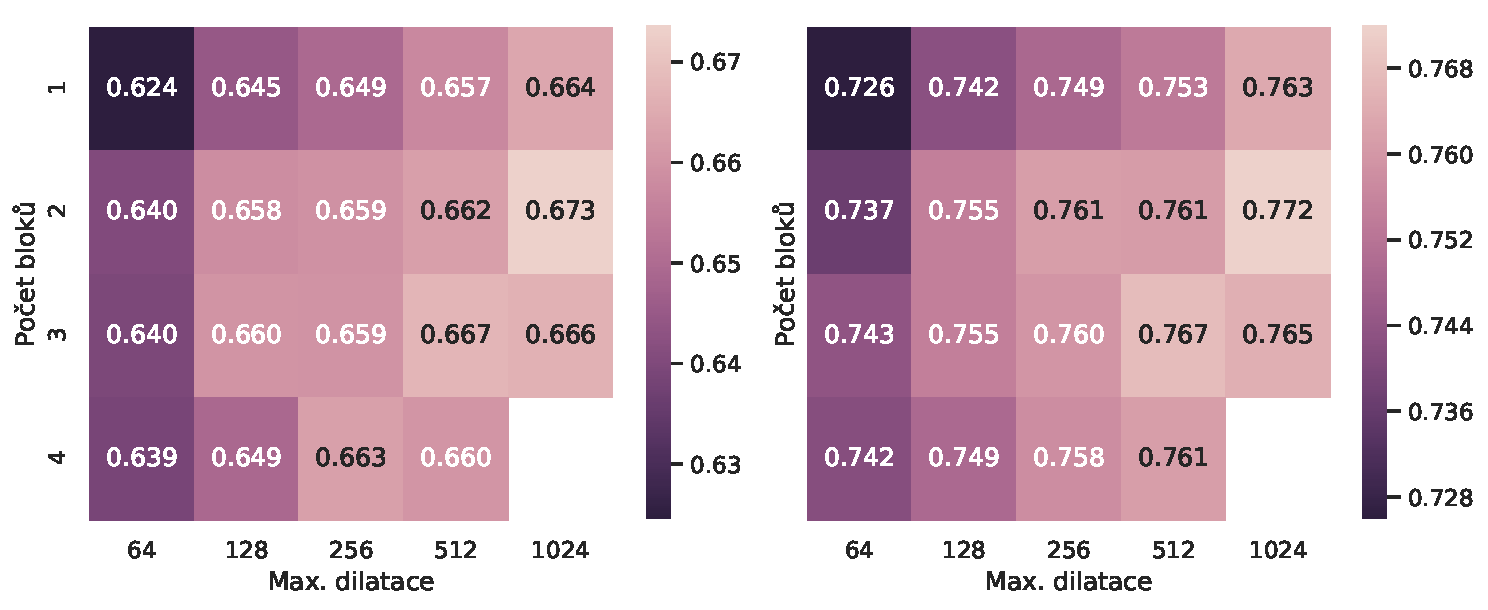
\includegraphics[scale=0.5]{../img/figures/wavenet_stacks_gridsearch.pdf}
\caption{Architektura WaveNet, systematické prohledávání počtu dilatačních vrstev a bloků, vlevo hodnoty RPA, vpravo RCA.}\label{obr:wavenet_stacks_gridsearch}
\end{figure}

Z tabulky lze dojít k pozorování, že přidávání počtu vrstev zvyšuje výslednou přesnost víceméně vždy, to neplatí o počtu bloků, u kterých se zdá, že nejvhodnější počet je 2. Pokud se zaměříme na srovnání výsledků s podobným dosahem, zdá se že výsledky jsou poměrně podobné, zejména pro širší dosahy, pro kratší se zdá lepší využít spíše více vrstev než více bloků.

\subsection{Vliv velikosti šířky kernelu dilatací}

Jiným způsobem, jak zvýšit velikost zpracovávaného kontextu, je volba velikosti šířky kernelu dilatací $n_{\mathrm{width}}$. Provedeme čtyři experimenty s různou šířkou. Šířka 2 je zvolena v původním článku z toho důvodu, že konvoluce se tím stávají \uv{kauzální} --- jejich výstup závisí pouze na vzorcích před nimi (viz obrázky \ref{obr:wavenet_conv}, \ref{obr:wavenet_dilated}). To je výhodné pro generativní úlohy, u kterých chceme, aby hodnota nového generovaného vzorku v audio signálu nezávisela na budoucích, zatím neexistujících vzorkách. U klasifikačních úloh takto omezeni nejsme, tudíž můžeme s nastavením experimentovat. 

\begin{table}[h!]
\centering
    \begin{tabular}{rrr}
    \toprule
    Šířka kernelu dilatací &   RPA &   RCA \\
    \midrule
                        2 & 0.649 & 0.754 \\
                        3 & 0.648 & 0.755 \\
                        4 & 0.656 & 0.759 \\
                        5 & 0.645 & 0.756 \\
    \bottomrule
    \end{tabular}
\caption{Architektura WaveNet, vliv velikosti šířky kernelu dilatací.}\label{tab:wavenet_dilation_width}
\end{table}

\begin{figure}[h]\centering
    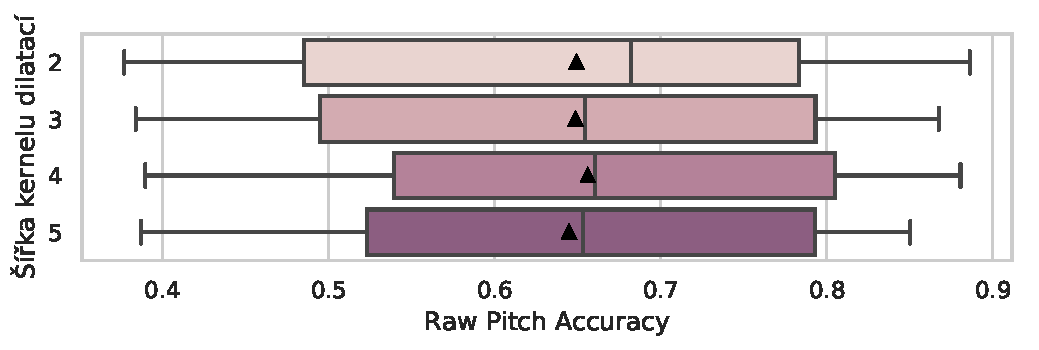
\includegraphics[scale=0.6]{../img/figures/wavenet_dilation_width.pdf}
\caption{Architektura WaveNet, vliv velikosti šířky kernelu dilatací.}\label{obr:wavenet_dilation_width}
\end{figure}

Z tabulky \ref{tab:wavenet_dilation_width} a grafu \ref{obr:wavenet_dilation_width} vyplývá, že tato síť při změnách šířky kernelu dilatace svou výslednou přesnost na validačních datech nemění.

\subsection{Vliv výstupní transformace skip propojení}

Volba transformace skip propojení se v článku týmu \cite{Oord2016} nediskutuje, \cite{Martak2018} také přejímají součet všech skip výstupů Vyzkoušíme proto dvě další možnosti práce se skip propojeními - výběr posledního skip propojení a dále konkatenace všech skip propojení do mnohakanálového výstupu. V případě výběru posledního či součtu jde o transformace, které lze popsat konvolucí nad konkatenovanými skip propojeními. Dalo by se tedy říct, že výběr a součet jsou v tomto případě speciálními případy konkatenace výstupů. Výběr poslední vrstvy také znamená, že nejsou potřeba předchozí skip propojení, což urychluje trénování.

\begin{table}[h!]
\centering
    \begin{tabular}{lrr}
    \toprule
    Transf. skip vrstev &   RPA &   RCA \\
    \midrule
            Konkatenace & 0.654 & 0.754 \\
            Poslední & 0.651 & 0.754 \\
                Součet & 0.646 & 0.753 \\
    \bottomrule
    \end{tabular}

\caption{Architektura WaveNet, vliv výstupní transformace skip propojení.}\label{tab:wavenet_skip_reduction}
\end{table}

\begin{figure}[h]\centering
    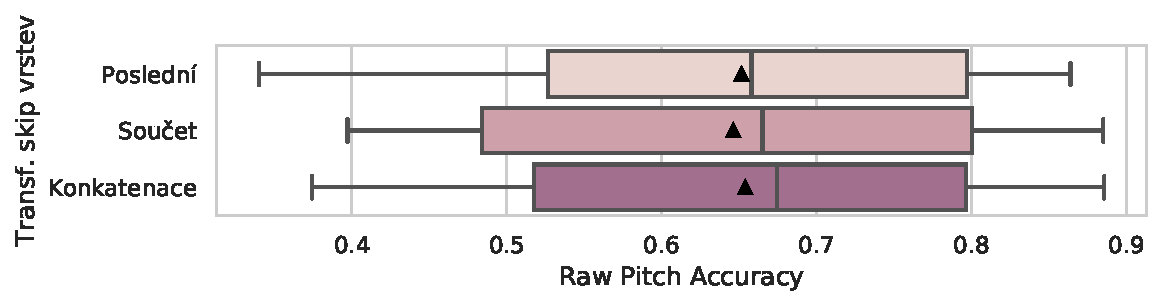
\includegraphics[scale=0.6]{../img/figures/wavenet_skip_reduction.pdf}
\caption{Architektura WaveNet, vliv výstupní transformace skip propojení.}\label{obr:wavenet_skip_reduction}
\end{figure}

Všechny tři transformace vedou ke stejné přesnosti. Síť tedy netěží z větších možností práce s dřívejšími vrstvami a nejdůležitejší informace se objevují až na vrchu bloků dilatovaných konvolucí.

\subsection{Vliv velikosti první konvoluce}

\cite{Oord2016} používá pro předzpracování zvukového signálu obvyklou konvoluci, nespecifikuje však její šířku. Veřejná implementace architektury WaveNet pracuje s šířkou 32 \footnote{\url{https://github.com/ibab/tensorflow-wavenet/blob/master/wavenet_params.json}}. \cite{Martak2018} používají šířku 2, čímž fakticky jen duplikují první dilatační vrstvu. První vrstva může sloužit jako banka filtrů, podobně jako první vrstva v architektuře CREPE, pro tento účel však musí být široká minimálně 512 vzorků, aby mohla zachytit periodu i té nejnižší frekvence ve výstupním rozsahu. 

\textcolor{red}{vizualizace první vrstvy? Co tam vlastně může být, když pomáhá šestnácti samplová konvoluce?}

\begin{table}[h!]
\centering
    \begin{tabular}{rrr}
    \toprule
    Velikost první vrstvy &   RPA &   RCA \\
    \midrule
                        0 & 0.648 & 0.755 \\
                        8 & 0.663 & 0.762 \\
                    16 & 0.661 & 0.765 \\
                    32 & 0.654 & 0.754 \\
                    64 & 0.643 & 0.756 \\
                    256 & 0.609 & 0.735 \\
                    1024 & 0.601 & 0.734 \\
    \bottomrule
    \end{tabular}
\caption{Architektura WaveNet, vliv velikosti první konvoluce.}\label{tab:wavenet_first_layer}
\end{table}

\begin{figure}[h]\centering
    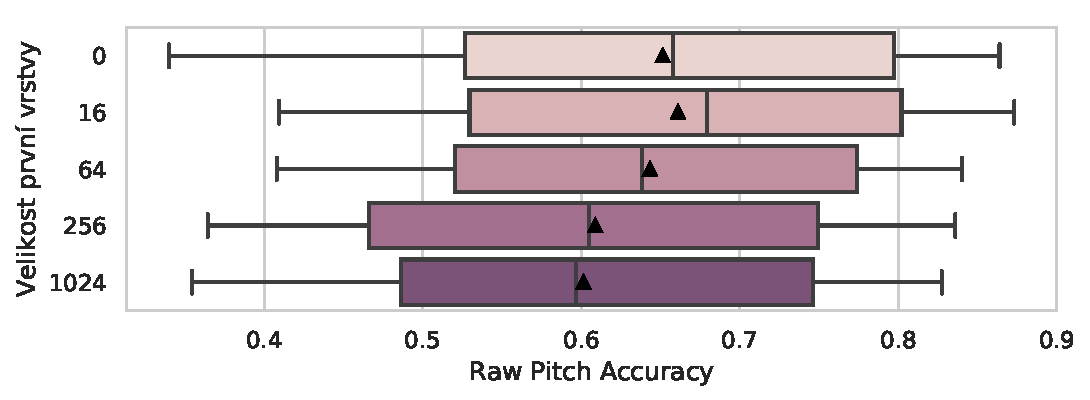
\includegraphics[scale=0.6]{../img/figures/wavenet_first_layer.pdf}
\caption{Architektura WaveNet, vliv velikosti první konvoluce.}\label{obr:wavenet_first_layer}
\end{figure}

\textcolor{red}{TODO: Dopsat vyhodnocení}

\subsection{Vliv návrhu posledních vrstev}

\begin{table}[h!]
\centering
\caption{Architektura WaveNet, vliv návrhu posledních vrstev.}\label{tab:wavenet_output_transform}
\end{table}

\begin{figure}[h]\centering
    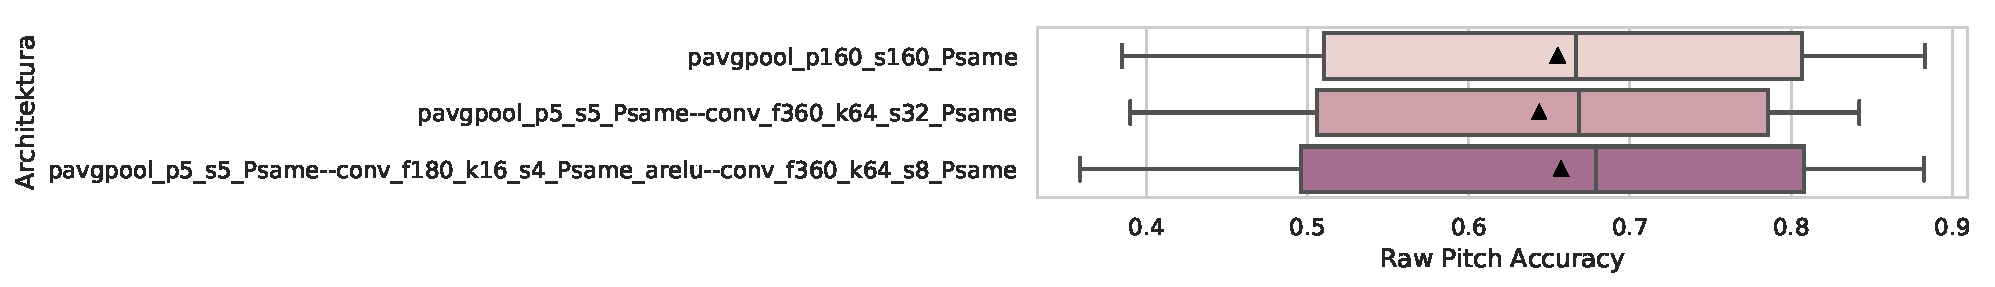
\includegraphics[scale=0.6]{../img/figures/wavenet_output_transform.pdf}
\caption{Architektura WaveNet, vliv návrhu posledních vrstev.}\label{obr:wavenet_output_transform}
\end{figure}


\chapter{Výsledky}\label{cha:vysledky}

V této kapitole shrnujeme výsledky vybraných architektur z kapitoly \nameref{cha:experimenty} na testovacích datech a provádíme kvantitativní a kvalitativní srovnání se state-of-the-art systémy pro extrakci melodie, představené v kapitole \nameref{cha:souvisejici}.

\section{Výběr testovaných modelů}

Pro srovnání jsme vybrali nejlepší natrénované modely z kapitoly \nameref{cha:experimenty} od každé testované architektury. Každou vybranou architekturu krátce popíšeme a v tabulce uvedeme nalezené nastavení hyperparametrů.

Všechny testované modely mají společnou reprezentaci cílového výstupu při trénování. Rozlišení diskretizace výšky noty je nastaveno na 5 hodnot na půltón, rozptyl distribuce výšky noty je nastaven na 0.18, na základě experimentů v sekci \nameref{sec:crepe}.

Modely byly trénovány pomocí grafické karty NVIDIA GeForce GTX 1070.

\subsection{Architektura CREPE}

Zvolený model dosáhl na validačních datech přesnosti odhadu výšky 0.682 a přesnosti odhadu výšky nezávisle na oktávě 0.783. Počet trénovatelných parametrů tohoto modelu je $2\,016\,350$. Proběhlo $360\,000$ iterací trénování. Trénování probíhalo přes dvě hodiny. Parametry vybrané architektury uvádíme v tabulce \ref{tab:crepe_hyperparams}.

\begin{table}[p]
\centering
\begin{tabular}{llll}
\toprule
Prohledávané parametry               &          & Ostatní parametry &         \\
Parametr                             & Hodnota  & Parametr          & Hodnota \\
\midrule
Multiplikační koef. kapacity         & 8        & Velikost dávky    & 32      \\
Šířka vstupního okna                 & 2048     & Iterace trénování & 360000         \\
Násobné rozlišení první vrstvy       & 6 vrstev & Learning rate     & 0.001   \\
\bottomrule
\end{tabular}
\caption{Nastavení architektury a hyperparametrů pro testovanou architekturu CREPE.}\label{tab:crepe_hyperparams}
\end{table}


\subsection{Architektura WaveNet}

Zvolený model dosáhl na validačních datech přesnosti odhadu výšky 0.673 a přesnosti odhadu výšky nezávisle na oktávě 0.768. Počet trénovatelných parametrů tohoto modelu je $5\,206\,524$. Proběhlo $360\,000$ iterací trénování. Trénování probíhalo téměř pět hodin. Parametry vybrané architektury uvádíme v tabulce \ref{tab:wavenet_hyperparams}.

\begin{table}[p]
\centering
\begin{tabular}{llll}
\toprule
Prohledávané parametry               &          & Ostatní parametry &         \\
Parametr                             & Hodnota  & Parametr          & Hodnota \\
\midrule
Velikost první konvoluce & 0      & Iterace trénování     & 100000 \\
Počet filtrů  & 16     & Velikost dávky    & 8      \\
Počet bloků            & 2     & Learning rate & 0.001       \\
Maximální dilatace         & 1024   &                &        \\
Transformace skip propojení & concat &                &        \\
\bottomrule
\end{tabular}
\caption{Nastavení architektury a hyperparametrů pro testovanou architekturu WaveNet.}\label{tab:wavenet_hyperparams}
\end{table}

\subsection{Architektura HCNN}

Pro úspěšnost modelů na validačních datech jsme se rozhodli porovnat dvě různé architektury HCNN. Architekturu s minimálním kontextem $5.8\,\rm ms$, dále nazývanou HCNN noctx, a architekturu, která uvažuje širší kontext, dále jen HCNN.

\subsubsection{HCNN noctx}

Zvolený model dosáhl na validačních datech přesnosti odhadu výšky 0.751 a přesnosti odhadu výšky nezávisle na oktávě 0.813. Počet trénovatelných parametrů tohoto modelu je $27\,857$. Proběhlo $100\,000$ iterací trénování. Trénování probíhalo 22 minut. Parametry vybrané architektury uvádíme v tabulce \ref{tab:hcnnnoctx_hyperparams}.

\begin{table}[p]
\centering
\begin{tabular}{llll}
\toprule
Prohledávané parametry               &          & Ostatní parametry &         \\
Parametr                             & Hodnota  & Parametr          & Hodnota \\
\midrule
Parametr \texttt{hop\_size} & 256       & Iterace trénování                       & 100000 \\
Kontext                & noctx         & Velikost dávky                      & 16     \\
Vstupní reprezentace   & HCQT       & Learning rate                   & 0.001  \\
Filtry, Bloky                 & 16, 8        & Dropout                          & 0.3    \\
Harmonická trans. & $\pm 12$, $\pm 19$ &  &       \\
\bottomrule
\end{tabular}
\caption{Nastavení architektury a hyperparametrů pro testovanou architekturu HCNN noctx.}\label{tab:hcnnnoctx_hyperparams}
\end{table}
\begin{table}[p]
\centering
\begin{tabular}{p{4.5cm}p{3cm}ll}
\toprule
Prohledávané parametry               &          & Ostatní parametry &         \\
Parametr                             & Hodnota  & Parametr          & Hodnota \\
\midrule
Parametr \texttt{hop\_size} & 256     & Iterace trénování                       & 100000 \\
Kontext            & 3\_last\_layers \_wavenet & Velikost dávky                      & 8      \\
Vstupní reprezentace    & Vícekan. HCQT & Learning rate                   & 0.001  \\
Filtry, Bloky & 16, 4      & Dropout                          & 0.3    \\
Harmonická trans. & $\pm 12$&   &       \\
Pst. augmentace       & 0.75    &                                  &        \\
\bottomrule
\end{tabular}
\caption{Nastavení architektury a hyperparametrů pro testovanou architekturu HCNN.}\label{tab:hcnn_hyperparams}
\end{table}

\subsubsection{HCNN}

Zvolený model dosáhl na validačních datech přesnosti odhadu výšky 0.755 a přesnosti odhadu výšky nezávisle na oktávě 0.828. Počet trénovatelných parametrů tohoto modelu je $23\,153$. Proběhlo $100\,000$ iterací trénování. Trénování probíhalo 75 minut. Parametry vybrané architektury uvádíme v tabulce \ref{tab:hcnn_hyperparams}.

\subsection{Detekce melodie}

Pro detekci melodie z vypočítané funkce salience jsme použili techniku práhování (thresholding). Pro odhad přítomnosti melodie nalezneme maximální hodnotu funkce salience v daném okamžiku --- pokud tato hodnota přesahuje jistý práh, daný časový okamžik se uvažuje jako obsahující melodii. Konkrétní nastavení práhu jsme určili na základě validačních dat pro každou metodu zvlášť. Tato metoda práhování je použita například také v práci \cite{Bittner2017}.

\section{Kvantitativní srovnání}

% , která je představuje evaluační páteř oboru a je každoročně pořádána pro nezávislé srovnávání metod úloh Music Information Retrieval

V tabulkách \ref{tab:vysledky_OA}, \ref{tab:vysledky_RPA}, \ref{tab:vysledky_RCA}, \ref{tab:vysledky_VR} a \ref{tab:vysledky_VFA} prezentujeme výsledky nově představovaných metod v porovnání s velmi silnými baseline metodami pro extrakci melodie. Jak uvádíme v kapitole \nameref{cha:souvisejici}, práce \cite{Salamon2012a} dosahuje spolu s prací \cite{Dressler2009} v průměru nejlepších výsledků v soutěži MIREX. Práce \cite{Bittner2017} a \cite{DBasaranSEssid2018} představují metody, které dosahují nejlepších výsledků na prozatím nejrozmanitějším datasetu MedleyDB. 

Pro srovnání metod používáme datasety ADC04, MIREX05train a ORCHSET, které jsme v práci vyhradili pouze pro testování. Také používáme testovací množiny datasetů MedleyDB a MDB-melody-synth, převzaté z prací \cite{Bittner2017} a \cite{DBasaranSEssid2018}, pro dataset WJazzD používáme vlastní testovací množinu. Metodika výběru příkladů do testovací množiny WJazzD je popsána v kapitole \nameref{cha:datasety}, všechny množiny jsou výčtem popsány v elektronické příloze.

V následujících tabulkách uvádíme standardní metriky, používané pro srovnání metod pro extrakci melodie, jde o metriky celkové přesnosti (OA), přesnosti odhadu výšky (RPA), přesnosti odhadu výšky nezávisle na oktávě (RCA), úplnosti detekce melodie (VR) a nesprávné detekce (VFA). Připomínáme, že metrika celkové přesnosti (OA) zahrnuje vyhodnocení odhadu výšky i vyhodnocení detekce melodie, zbylé metriky měří úspěšnost pouze jedné z obou podúloh. K vyhodnocování používáme knihovnu \texttt{mir\_eval}, která poskytuje transparentní a standardizovaný způsob výpočtu metrik pro úlohy oboru Music Information Retrieval.

\begin{table}[p]
\centering
\scalebox{1.0}{%
\begin{tabular}{lrrrrrr}
\toprule
Metoda & ADC04 & \shortstack[r]{MDB-m-s\\ test} & \shortstack[r]{MIREX05\\train.} & \shortstack[r]{MDB\\test} & \shortstack[r]{ORCH-\\SET} & \shortstack[r]{WJazzD\\test} \\
\midrule
    Salamon &         0.714 &           0.527 &          0.715 &         0.519 &        0.235 &        0.667 \\
    Bittner &         0.716 &           0.633 &          0.702 &         0.611 &        0.407 &        0.692 \\
    Basaran &         0.669 &   \textbf{0.689}&          0.734 &         0.640 &\textbf{0.483}&        0.700 \\
\arrayrulecolor{black!30}\midrule
      CREPE &         0.590 &           0.562 &          0.652 &         0.502 &        0.248 &        0.671 \\
    WaveNet &         0.681 &           0.528 &          0.649 &         0.503 &        0.256 &        0.648 \\
 HCNN noctx & \textbf{0.737}&           0.626 &          0.723 &         0.635 &        0.439 &        0.715 \\
       HCNN &         0.726 &           0.661 &  \textbf{0.755}& \textbf{0.652}&        0.459 &\textbf{0.725} \\
\arrayrulecolor{black}\bottomrule
\end{tabular}
}%
\caption{Výsledky celkové přesnosti (Overall Accuracy). Vyznačené výsledky jsou pro daný dataset nejvyšší z porovnávaných v rámci daného datasetu.}\label{tab:vysledky_OA}
\end{table}

\begin{table}[p]
\centering
\scalebox{1.0}{%
\begin{tabular}{lrrrrrr}
\toprule
Metoda & ADC04 & \shortstack[r]{MDB-m-s\\ test} & \shortstack[r]{MIREX05\\train.} & \shortstack[r]{MDB\\test} & \shortstack[r]{ORCH-\\SET} & \shortstack[r]{WJazzD\\test} \\
\midrule
    Salamon &          0.767 &           0.514 &          0.761 &         0.526 &         0.281 &        0.693 \\
    Bittner &          0.814 &           0.606 &          0.807 &         0.670 &         0.519 &        0.774 \\
    Basaran &          0.793 &   \textbf{0.733}&          0.798 &         0.706 & \textbf{0.635}&        0.767 \\
\arrayrulecolor{black!30}\midrule
      CREPE &          0.794 &           0.550 &          0.779 &         0.616 &         0.408 &        0.782 \\
    WaveNet &          0.796 &           0.528 &          0.792 &         0.595 &         0.345 &        0.759 \\
 HCNN noctx &          0.827 &           0.647 &          0.833 &         0.701 &         0.511 &        0.805 \\
       HCNN &  \textbf{0.841}&           0.654 &  \textbf{0.851}& \textbf{0.715}&         0.535 &\textbf{0.806}\\
\arrayrulecolor{black}\bottomrule
\end{tabular}
}%
\caption{Výsledky přesnosti odhadu výšky (Raw Pitch Accuracy). Vyznačené výsledky jsou pro daný dataset nejvyšší z porovnávaných v rámci daného datasetu.}\label{tab:vysledky_RPA}
\end{table}

\begin{table}[p]
\centering
\scalebox{1.0}{%
\begin{tabular}{lrrrrrr}
\toprule
Metoda & ADC04 & \shortstack[r]{MDB-m-s\\ test} & \shortstack[r]{MIREX05\\train.} & \shortstack[r]{MDB\\test} & \shortstack[r]{ORCH-\\SET} & \shortstack[r]{WJazzD\\test} \\
\midrule
    Salamon &        0.807 &        0.639 &        0.805 &         0.659 &         0.568 &             0.757 \\
    Bittner &        0.855 &        0.666 &        0.824 &         0.735 &         0.694 &             0.785 \\
    Basaran &        0.820 &\textbf{0.766}&        0.807 &         0.757 & \textbf{0.776}&             0.776 \\
\arrayrulecolor{black!30}\midrule
      CREPE &        0.851 &        0.617 &        0.810 &         0.714 &         0.607 &             0.808 \\
    WaveNet &        0.843 &        0.597 &        0.828 &         0.703 &         0.564 &             0.793 \\
 HCNN noctx &        0.862 &        0.699 &        0.845 &         0.767 &         0.683 &     \textbf{0.821}\\
       HCNN &\textbf{0.880}&        0.716 &\textbf{0.863}& \textbf{0.781}&         0.732 &             0.820 \\
\arrayrulecolor{black}\bottomrule
\end{tabular}
}%
\caption{Výsledky přesnosti odhadu výšky nezávisle na oktávě (Raw Chroma Accuracy). Vyznačené výsledky jsou pro daný dataset nejvyšší z porovnávaných v rámci daného datasetu.}\label{tab:vysledky_RCA}
\end{table}


\begin{table}[h]
\centering
\scalebox{1.0}{%
\begin{tabular}{lrrrrrr}
\toprule
Metoda & ADC04 & \shortstack[r]{MDB-m-s\\ test} & \shortstack[r]{MIREX05\\train.} & \shortstack[r]{MDB\\test} & \shortstack[r]{ORCH-\\SET} & \shortstack[r]{WJazzD\\test} \\
\midrule
\arrayrulecolor{black!30}\midrule
    Salamon &          0.774 &       \bf{0.729}&      \bf{0.841}&         0.705 &       0.603 &       0.794 \\
    Bittner &          0.796 &           0.638 &          0.796 &         0.675 &       0.614 &       0.846 \\
    Basaran &          0.732 &           0.704 &          0.713 &         0.676 &       0.605 &       0.841 \\
      CREPE &          0.584 &           0.431 &          0.576 &         0.449 &       0.326 &       0.680 \\
    WaveNet &          0.765 &           0.595 &          0.747 &         0.618 &       0.494 &       0.784 \\
 HCNN noctx &      \bf{0.806}&           0.684 &          0.824 &         0.728 &   \bf{0.729}&   \bf{0.880}\\
       HCNN &          0.794 &           0.692 &          0.836 &     \bf{0.741}&       0.721 &       0.872 \\
\arrayrulecolor{black}\bottomrule
\end{tabular}
}%
\caption{Výsledky úplnosti detekce (Voicing Recall).}\label{tab:vysledky_VR}
\end{table}
\begin{table}[h]
\centering
\scalebox{1.0}{%
\begin{tabular}{lrrrrrr}
\toprule
Metoda & ADC04 & \shortstack[r]{MDB-m-s\\ test} & \shortstack[r]{MIREX05\\train.} & \shortstack[r]{MDB\\test} & \shortstack[r]{ORCH-\\SET} & \shortstack[r]{WJazzD\\test} \\
\midrule
\arrayrulecolor{black!30}\midrule
    Salamon &      \bf{0.103}&           0.394 &          0.263 &         0.300 &        0.385 &       0.271 \\
    Bittner &          0.278 &           0.273 &          0.308 &         0.306 &        0.490 &       0.333 \\
    Basaran &          0.188 &           0.271 &      \bf{0.160}&         0.290 &        0.407 &       0.274 \\
      CREPE &          0.178 &       \bf{0.252}&          0.171 &     \bf{0.243}&    \bf{0.235}&   \bf{0.213}\\
    WaveNet &          0.311 &           0.383 &          0.387 &         0.397 &        0.426 &       0.370 \\
 HCNN noctx &          0.246 &           0.312 &          0.336 &         0.333 &        0.535 &       0.339 \\
       HCNN &          0.222 &           0.258 &          0.278 &         0.310 &        0.511 &       0.300 \\
\arrayrulecolor{black}\bottomrule
\end{tabular}
}%
\caption{Výsledky nesprávné detekce (Voicing False Alarm). Nižší hodnota je lepší.}\label{tab:vysledky_VFA}
\end{table}


\subsection{Popis výsledků}

Metody HCNN a HCNN noctx překonávají srovnávané algoritmy v metrikách celkové přesnosti (OA), přesnosti odhadu výšky (RPA) a přesnosti odhadu výšky nezávisle na oktávě (RCA) na datasetech ADC04, MIREX05train a WJazzD. Metoda HCNN pak překonává všechny srovnávané přístupy i na datasetu MedleyDB. Na obrázku \ref{obr:final_medleydb} porovnáváme rozdělení dosažených výsledků na datasetu MedleyDB, na uvedeném krabicovém grafu lze navíc porovnat rozptyl výsledků. V metrice RCA metody HCNN dosahují menší variability na sadě testovacích příkladů. Na zbylých datasetech MDB-melody-synth a ORCHSET překonává architektura HCNN ve všech uvažovaných metrikách pouze práce \cite{Salamon2012a} a \cite{Bittner2017}.

Co se týče zbylých architektur CREPE a WaveNet, v metrikách přesnosti odhadu výšky (RPA) a přesnosti odhadu výšky nezávisle na oktávě (RCA) na téměř všech testovacích datasetech překonávají metodu \cite{Salamon2012a}, která není založena na strojovém učení. Výsledky v porovnání s HCNN, \cite{Bittner2017} a \cite{DBasaranSEssid2018} jsou však až na výjimky nižší.

Podle očekávání na základě výsledků ze soutěže MIREX se na datasetu ORCHSET výsledky algoritmů liší nejvíce, v některých případech až o desítky procent. Jak popisujeme v kapitole \nameref{cha:datasety}, dataset je složen z orchestrálních nahrávek a kvůli vysokému stupni polyfonie a rozmanitým kombinacím barev nástrojů se jedná pro metody extrakce melodie o velmi náročný materiál. Naopak nejblíže, zejména v metrikách RPA a RCA, jsou si výsledky na datasetech ADC04, MIREX05train a WJazzD. Výňatky v těchto datasetech často obsahují velmi zřetelnou melodii a v porovnání s datasetem MedleyDB je jejich hudební obsah žánrově homogenní.

Vzhledem k dosaženým výsledkům, jednoduchosti sítí a rychlému trénování považujeme návrh architektury HCNN jako nadějný podklad pro navazující práci. Abychom mohli uvedené výsledky interpretovat, provedeme nejprve také kvalitativní srovnání algoritmů. 

% \textcolor{red}{dopsat}
% - basaran má vyhlazování, bittnerová ne, tu překovávám vždy (porovnat velikosti oken)

\begin{figure}[h]\centering
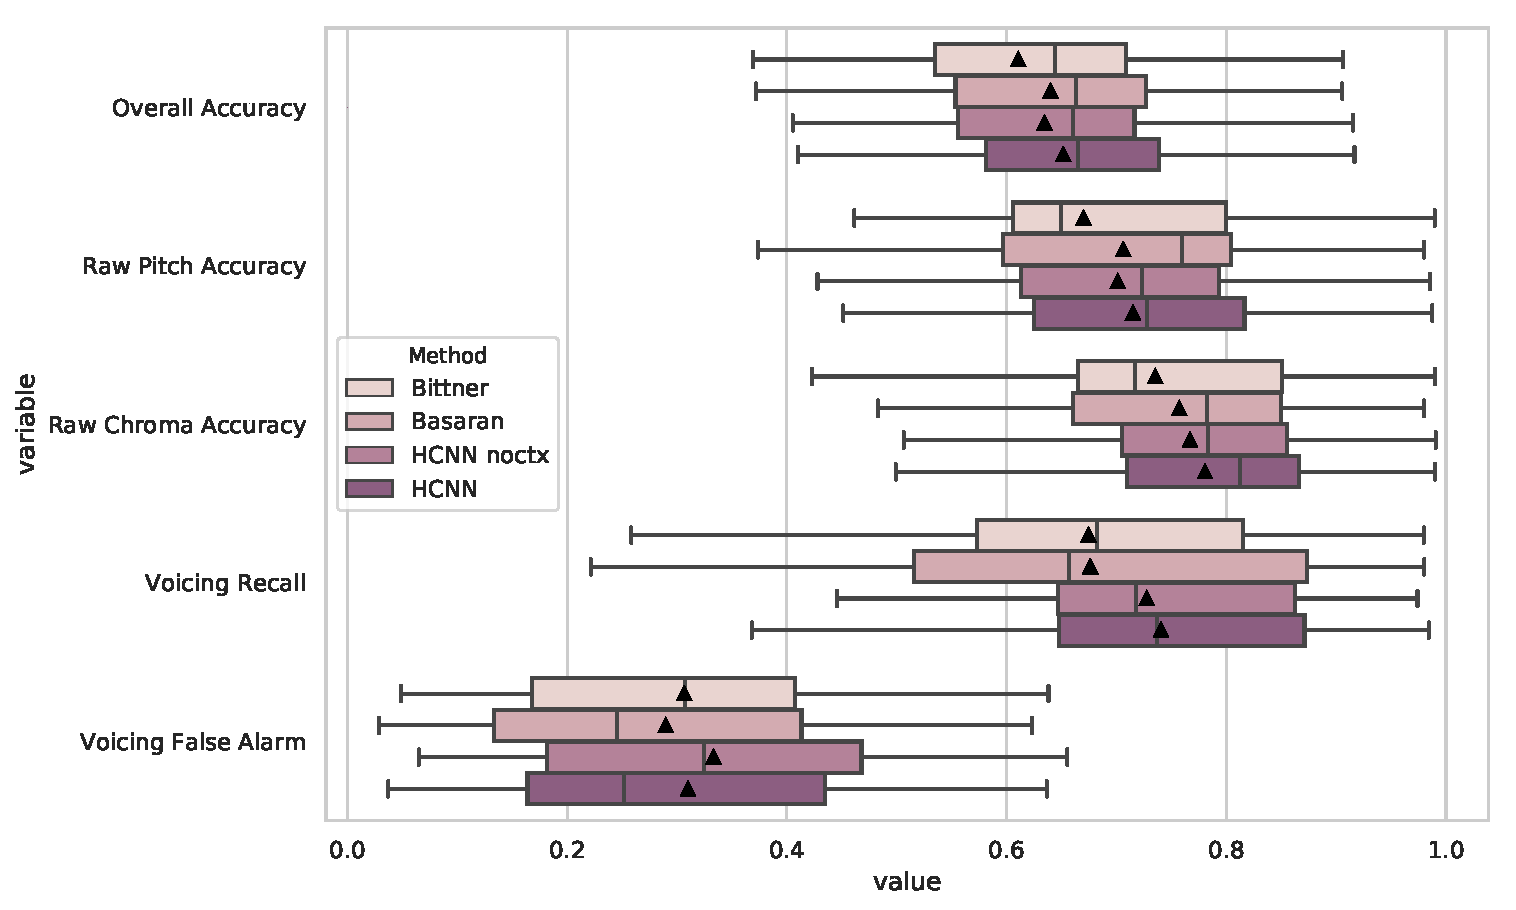
\includegraphics[width=\textwidth,height=\textheight,keepaspectratio]{../img/final_medleydb}
\caption{Výsledky nejúspěšnějších metod na datasetu MedleyDB}
\label{obr:final_medleydb}
\end{figure}

\section{Kvalitativní srovnání}

Na základě kvantitativního vyhodnocení vybíráme metody Bittnerové a Basarana pro podrobnější srovnání na jednotlivých příkladech. Z testovaných architektur pak vybíráme obě varianty HCNN. V následujících srovnáních se soustředíme na odhad výšky, proto v obrázcích zobrazujeme pouze části odhadů, ve kterých podle referenční anotace melodie zní. Obrázky jsou bez tohoto zjednodušení příliš komplikované a v práci detekci melodie řešíme pouze okrajově. Metodika výběru kvalitativních příkladů spočívala v hledání skladeb, ve kterých se odhady jednotlivých algoritmů vzájemně nejvíce lišily s nadějí, že právě tyto příklady budou nejlépe ilustrovat limity porovnávaných metod. Vybíráme ale také příklady, které jsou napříč metodami pro odhad melodie obtížné a také ukázku snadno analyzovatelného vstupu. Legenda barev použitých ve všech následujících obrázcích je vysvětlena na obrázku \ref{obr:legenda}
 Pro srovnání vybíráme příklady, ve kterých se výstupy sítí nejvíce lišily.

\begin{figure}[h]\centering
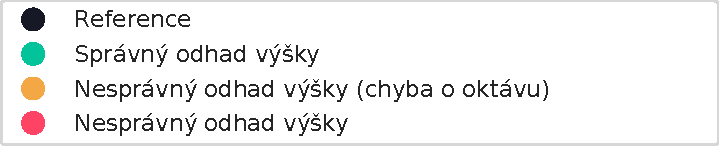
\includegraphics[scale=0.75]{../img/legenda}
\caption{Legenda pro následující kvalitativní srovnání.}
\label{obr:legenda}
\end{figure}

\begin{figure}[h]\centering
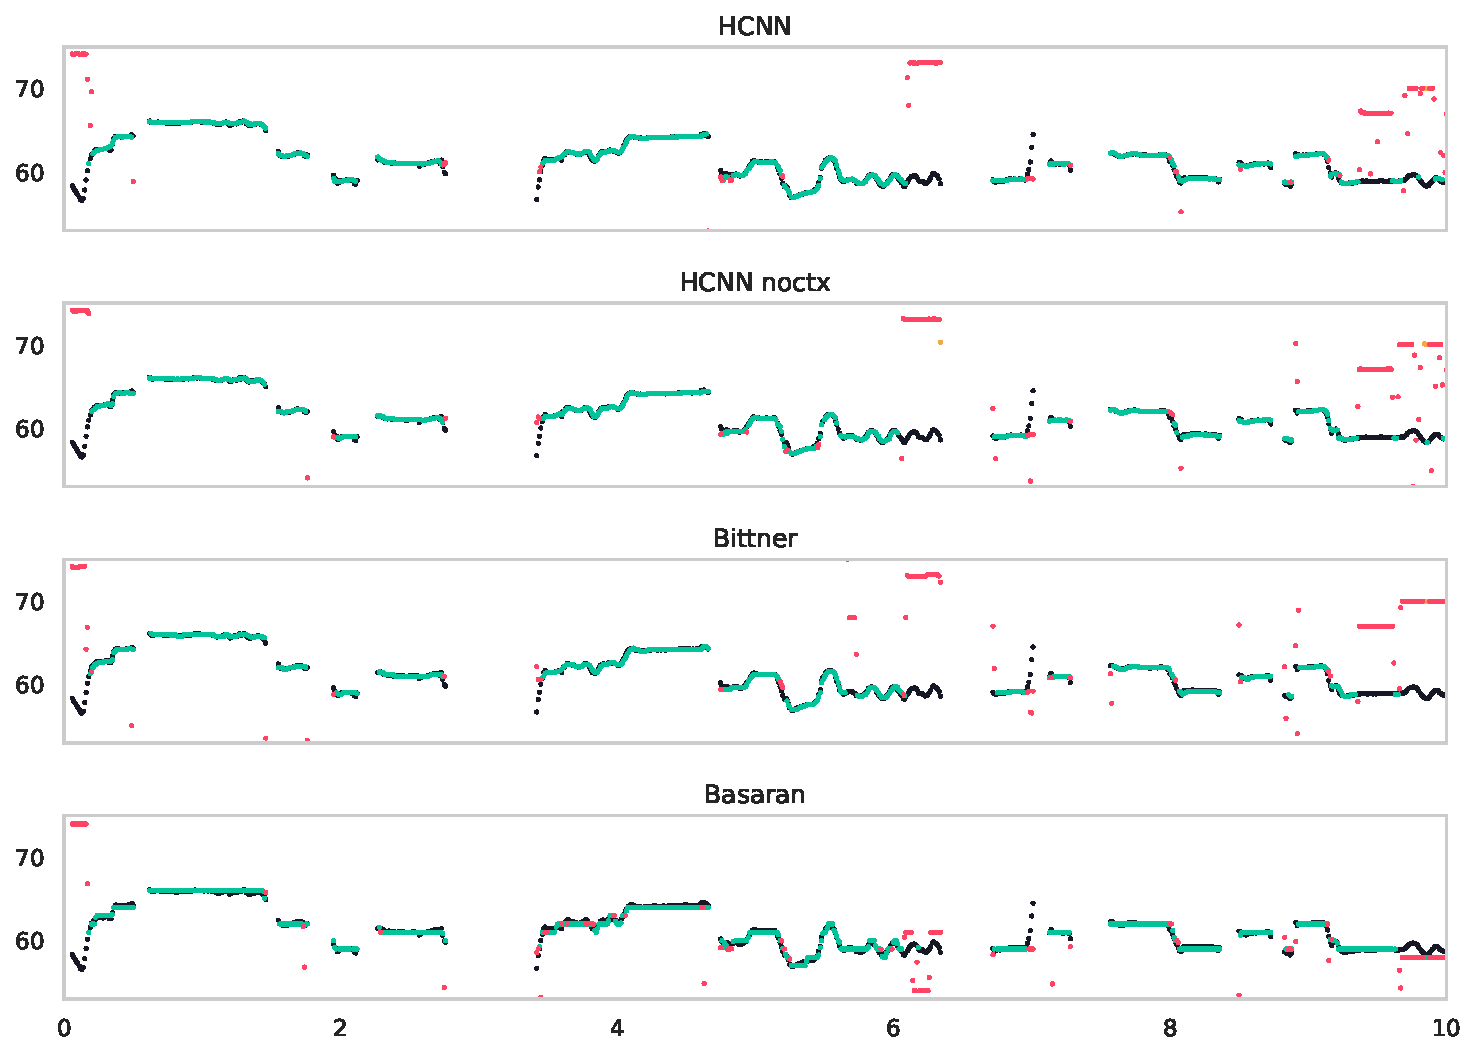
\includegraphics[width=\textwidth,height=\textheight,keepaspectratio]{../img/vysledky/mirex05_train01}
\caption{Příklad s vysokou úspěšností přepisu \texttt{train01} z datasetu MIREX05\-train, se kterým je čtenář seznámen z úvodu práce.}
\label{obr:mirex05_train01}
\end{figure}

Na obrázku \ref{obr:mirex05_train01} můžeme vidět výsledky metod spuštěných na popové nahrávce, ve které melodii nese hlas zpěvačky. Napříč metodami je přepis této nahrávky, kterou uvádíme v úvodu práce, velmi spolehlivý, přesnost odhadu výšky se pohybuje mezi 0.86 a 0.89. Protože v následujících srovnáních ukazujeme zejména chyby přepisu a metody porovnáváme na obtížných příkladech, nechceme, aby si po přečtení sekce čtenář odnesl, že existující metody přepisu nefungují. Proto uvádíme tento příklad (obr. \ref{obr:mirex05_train01}) jako pozitivní ukázku toho, že na obvyklých vstupních datech všechny porovnávané metody fungují velmi dobře.


% \begin{table}[h]
% \centering

%     \begin{tabular}{ll}
%     \toprule
%     Metrika (Metoda) & train10 \\
%     \midrule
%           RPA (HCNN) &   0.917 \\
%           RCA (HCNN) &   0.934 \\
%       RPA (Bittner) &   0.863 \\
%       RCA (Bittner) &   0.868 \\
%       RPA (Basaran) &   0.512 \\
%       RCA (Basaran) &   0.572 \\
%     \bottomrule
%     \end{tabular}

% \caption{Přesnost metod na testovacím souboru \texttt{train10} z datasetu MIREX05.}\label{tab:mirex05_train10}
% \end{table}
\begin{figure}[h]\centering
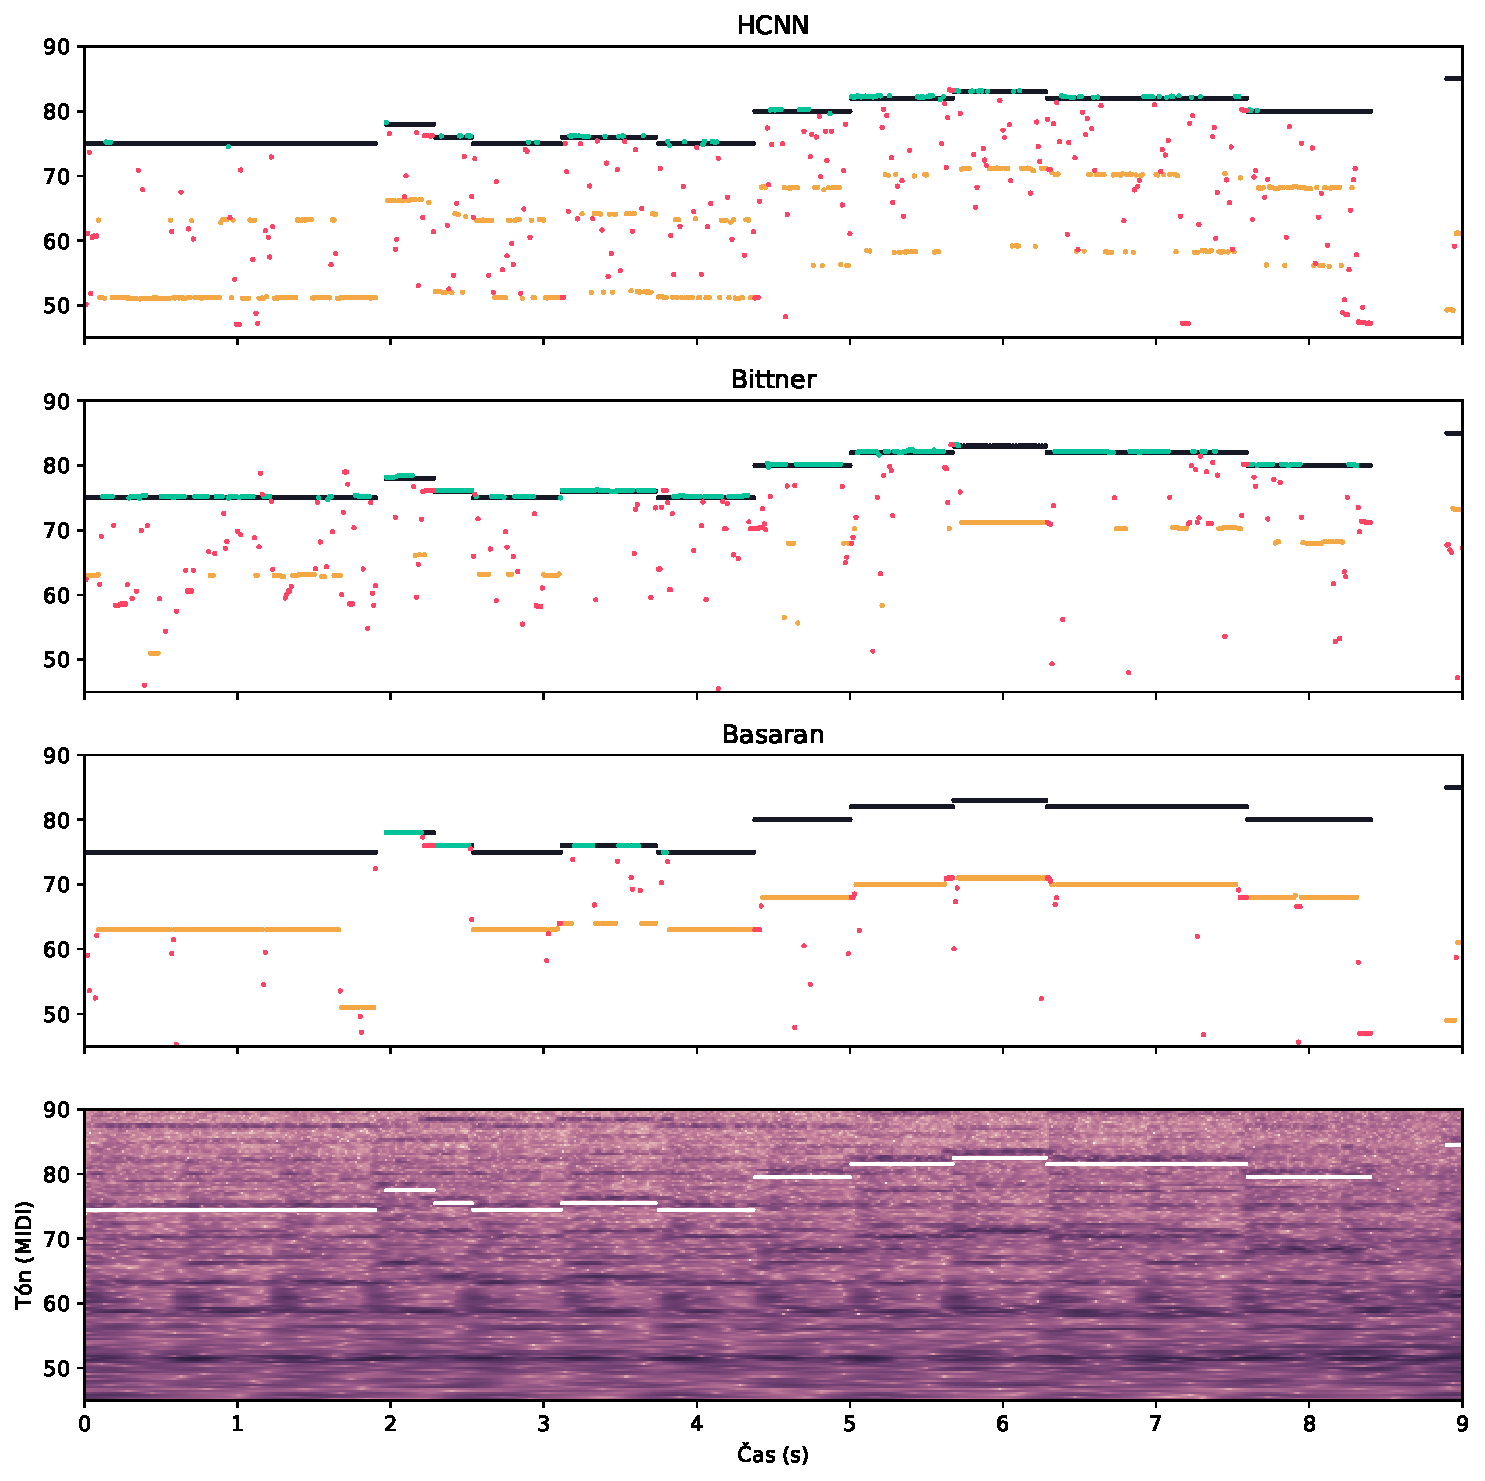
\includegraphics[width=\textwidth,height=\textheight,keepaspectratio]{../img/vysledky/orchset_Musorgski-Ravel-PicturesExhibition-ex6}
\caption{Výstup metod na testovacím souboru \texttt{Musorg\allowbreak{}ski\-Ravel\-Pictures\allowbreak{}Exhibition\-ex6} z datasetu ORCHSET.}
\label{obr:orchset_Musorgski-Ravel-PicturesExhibition-ex6}
\end{figure}

\begin{figure}[h]\centering
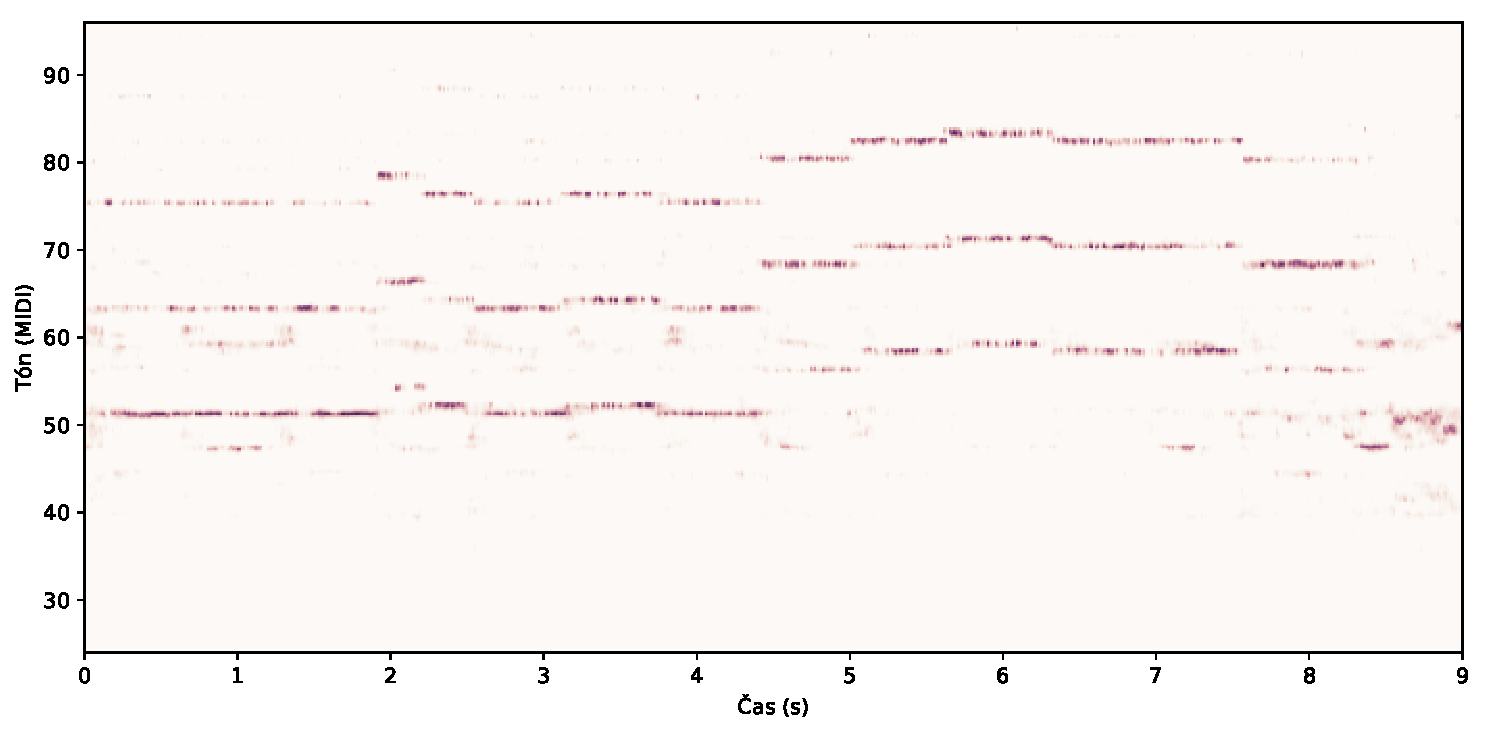
\includegraphics[scale=0.4]{../img/vysledky/orchset_Musorgski-Ravel-PicturesExhibition-ex6_salience}
\caption{Výstupní salience metody HCNN na testovacím souboru \texttt{Musorg\allowbreak{}ski\-Ravel\-Pictures\allowbreak{}Exhibition\-ex6} z datasetu ORCHSET.}
\label{obr:orchset_Musorgski-Ravel-PicturesExhibition-ex6_salience}
\end{figure}

Největší slabinou sítě HCNN noctx se stala podle očekávání časová kontinuita odhadů. Protože tato síť pro odhad výšek uvažuje vždy pouze $5.8\,\rm ms$ vstupu a po vytvoření funkce salience na odhady tónů neaplikujeme žádné způsoby vyhlazování, odhady jednotlivých časových oken na sebe nenavazují. To se nejeví jako zásadní problém v případech, kdy ve skladbě melodii nenese více hlasů v souzvuku (viz výstup \ref{obr:mirex05_train01}, \ref{obr:mirex05_train10}). U některých orchestrálních skladeb však vzniká problém, například pokud melodii nese zároveň sekce smyčců a dechů v různých oktávách. Jak můžeme vidět na výstupu algoritmů \ref{obr:orchset_Musorgski-Ravel-PicturesExhibition-ex6}, HCNN noctx pak \uv{přeskakuje} mezi oktávami. Problém je také dobře vidět na výstupní funkci salience \ref{obr:orchset_Musorgski-Ravel-PicturesExhibition-ex6_salience}, na které vidíme tři totožné kontury posunuté o oktávu. Mírné zlepšení tohoto problému vidíme na výstupech metod HCNN a \cite{Bittner2017}, které sice také nijak výsledek salienční funkce nezpracovávají, na druhou stranu pro její výpočet uvažují delší okna délky $162\,\rm ms$ v případě HCNN a $150\,\rm ms$ v případě metody Bittner. Na obrázku \ref{obr:orchset_Musorgski-Ravel-PicturesExhibition-ex6} vidíme, že množství odhadů těchto metod, je často chybný pouze kvůli nesprávně určené oktávě --- díky většímu kontextu může metoda vybrat v čase navazující odhady a proto tyto výstupy obsahují méně velmi krátkých chybných úseků. Metoda týmu \cite{DBasaranSEssid2018} odhad výšky tónů vyhlazuje pomocí rekurentní architektury GRU, jejich výstup proto obsahuje nejméně skoků, jelikož metoda uvažuje celý kontext skladby, nikoli jen okno omezené délky. Použití rekurentní sítě díky tomu dovoluje zachytit ještě dlouhodobější závislosti a výstupní kontura pak často obsahuje nejmenší množství velmi krátkých, chybných skoků mimo hlavní melodii, které se na obrázku \ref{obr:orchset_Musorgski-Ravel-PicturesExhibition-ex6} hojně vyskytují u metod bez vyhlazování. Na obrázku \ref{obr:orchset_Musorgski-Ravel-PicturesExhibition-ex6} proto vidíme, že metoda \cite{DBasaranSEssid2018} se drží při odhadu jedné oktávy a přesto, že je tato oktáva zvolena špatně, výsledný přepis je koherentní.

% Také je celkový průběh výsledné kontury u této metody častěji . Další výraznou slabinu jsme z analýzy jednotlivých výstupů sítí neregistrovali. U výstupů, ve kterých se sítě nejvíce lišily, byl tento rozdíl nejčastěji způsoben právě těmito diskontinuitami, případně pak zachycením jiného než hlavního nástroje v pozadí. Největší rozdíly ve výsledcích jsou proto na datasetu ORCHSET, ve kterém je výskyt polyfonie nejčastější. 


% \begin{table}[h]
% \centering

%     \begin{tabular}{ll}
%     \toprule
%     Metrika (Metoda) & Musorgski-Ravel-PicturesExhibition-ex6 \\
%     \midrule
%           RPA (HCNN) &                                  0.125 \\
%           RCA (HCNN) &                                  0.725 \\
%       RPA (Bittner) &                                  0.397 \\
%       RCA (Bittner) &                                  0.826 \\
%       RPA (Basaran) &                                  0.040 \\
%       RCA (Basaran) &                                  0.914 \\
%     \bottomrule
%     \end{tabular}

% \caption{Přesnost metod na testovacím souboru \texttt{Musorgski-Ravel-PicturesExhibition-ex6} z datasetu ORCHSET.}\label{tab:orchset_Musorgski-Ravel-PicturesExhibition-ex6}
% \end{table}

\begin{figure}[h]\centering
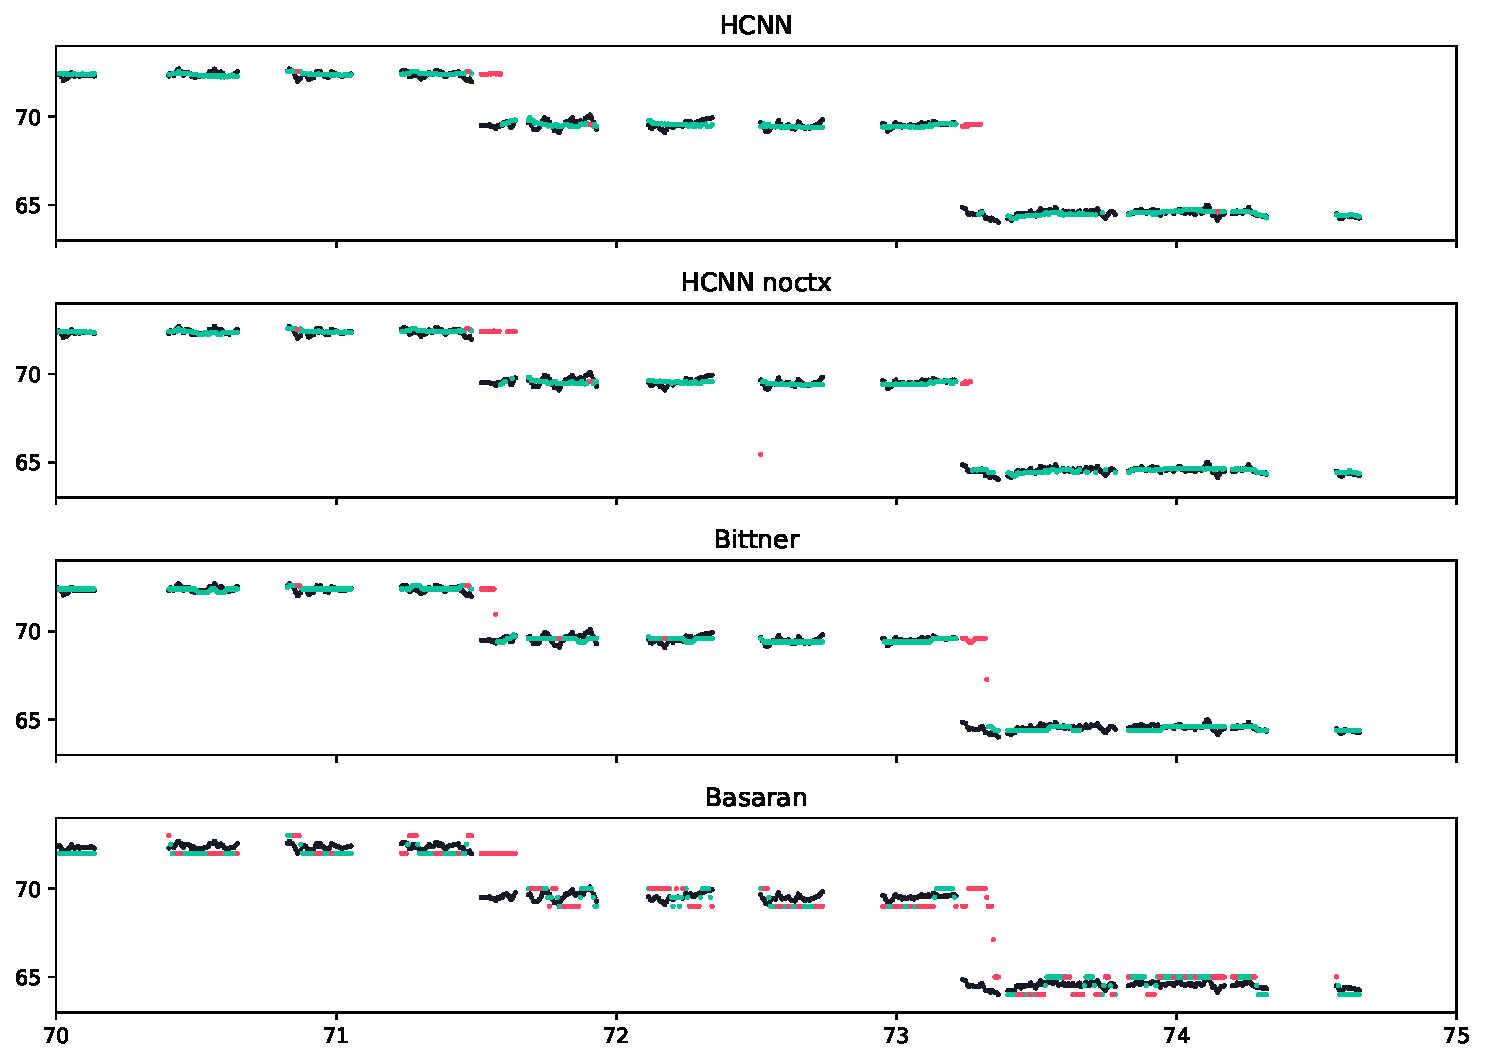
\includegraphics[width=\textwidth,height=\textheight,keepaspectratio]{../img/vysledky/wjazzd_CannonballAdderley_SoWh}
\caption{Detail přepisu metod na testovacím souboru \texttt{Cannonball\allowbreak{}Adderley\allowbreak{}\_\allowbreak{}So\allowbreak{}What} z datasetu WJazzD.}
\label{obr:wjazzd_CannonballAdderley_SoWhat_detail}
\end{figure}


Basaranova metoda pro tuto koherenci výsledných kontur však obětovala frekvenční přesnost znějících výšek tónů, frekvenční rozlišení této metody je totiž na úrovni jednoho půltónu. Jak jsme již prezentovali v kapitole \nameref{cha:experimenty}, výstup metod kvantizovaný na půltóny obsahuje množství chyb navíc, jelikož často selhává v zachycení frekvenčních modulací. Na obrázku \ref{obr:wjazzd_CannonballAdderley_SoWhat_detail} vidíme další limitaci takového výstupu --- pokud je obsah skladby laděný podle jiného referenčního tónu než jaký byl použit pro trénování sítě, znějící tóny vycházejí výškou \uv{mezi} výstupní složky. Z tabulky \ref{tab:wjazzd_CannonballAdderley_SoWhat} je pak zřejmé, že kvůli této kvantizaci síť nedosahuje srovnatelných výsledků, přestože na jiných, žánrově shodných datech, které jsou laděny na správný referenční tón, podává kompetitivní výsledky. Limitace se proto týká zejména jazzových nahrávek pocházejících z období před rokem 1955, před zavedením referenčního tónu A4=440Hz ve standardu ISO16.
\begin{table}[h]
\centering
\begin{tabular}{ll}
\toprule
 Metrika (Metoda) & CannonballAdderley\_SoWhat \\
\midrule
       RPA (HCNN) &                     0.850 \\
 RPA (HCNN noctx) &                     0.848 \\
    RPA (Bittner) &                     0.828 \\
    RPA (Basaran) &                     0.653 \\
\bottomrule
\end{tabular}


% \begin{figure}[h]\centering
% 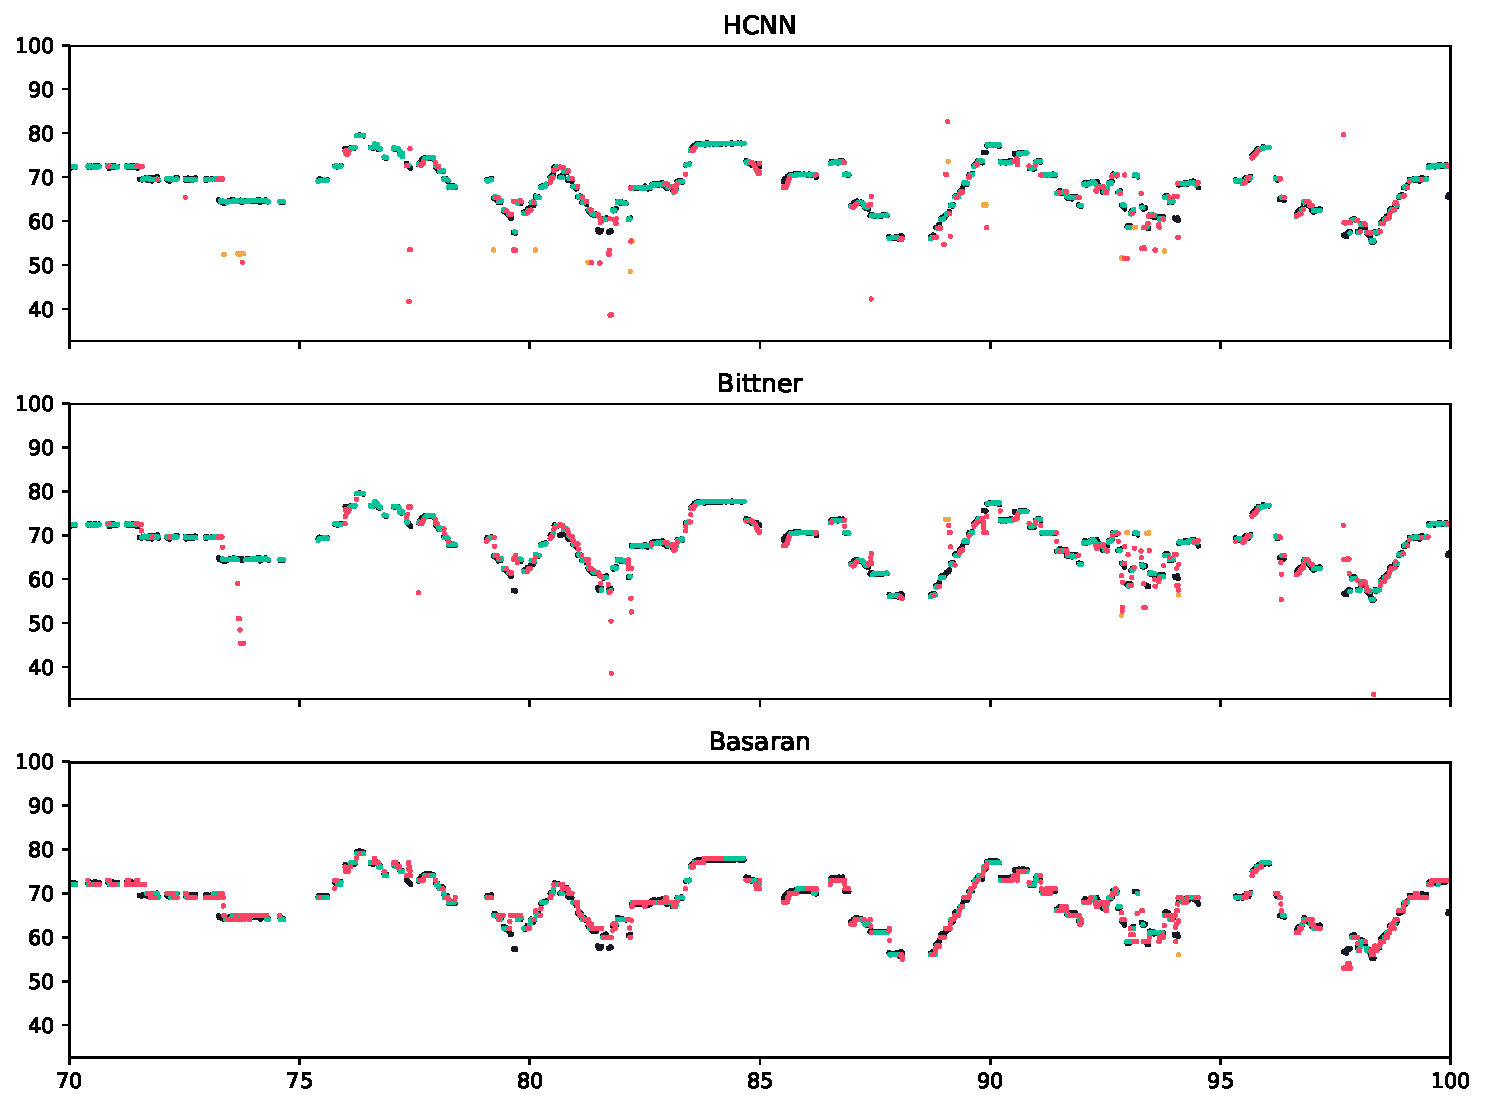
\includegraphics[width=\textwidth,height=\textheight,keepaspectratio]{../img/vysledky/wjazzd_CannonballAdderley_SoWhat}
% \caption{Výstup metod na testovacím souboru \texttt{CannonballAdderley\_SoWhat} z datasetu WJazzD.}
% \label{obr:wjazzd_CannonballAdderley_SoWhat}
% \end{figure}

\caption{Přesnost metod na testovacím souboru \texttt{Cannonball\allowbreak{}Adderley\allowbreak{}\_So\allowbreak{}What} z datasetu WJazzD.}\label{tab:wjazzd_CannonballAdderley_SoWhat}
\end{table}


\begin{figure}[p]\centering
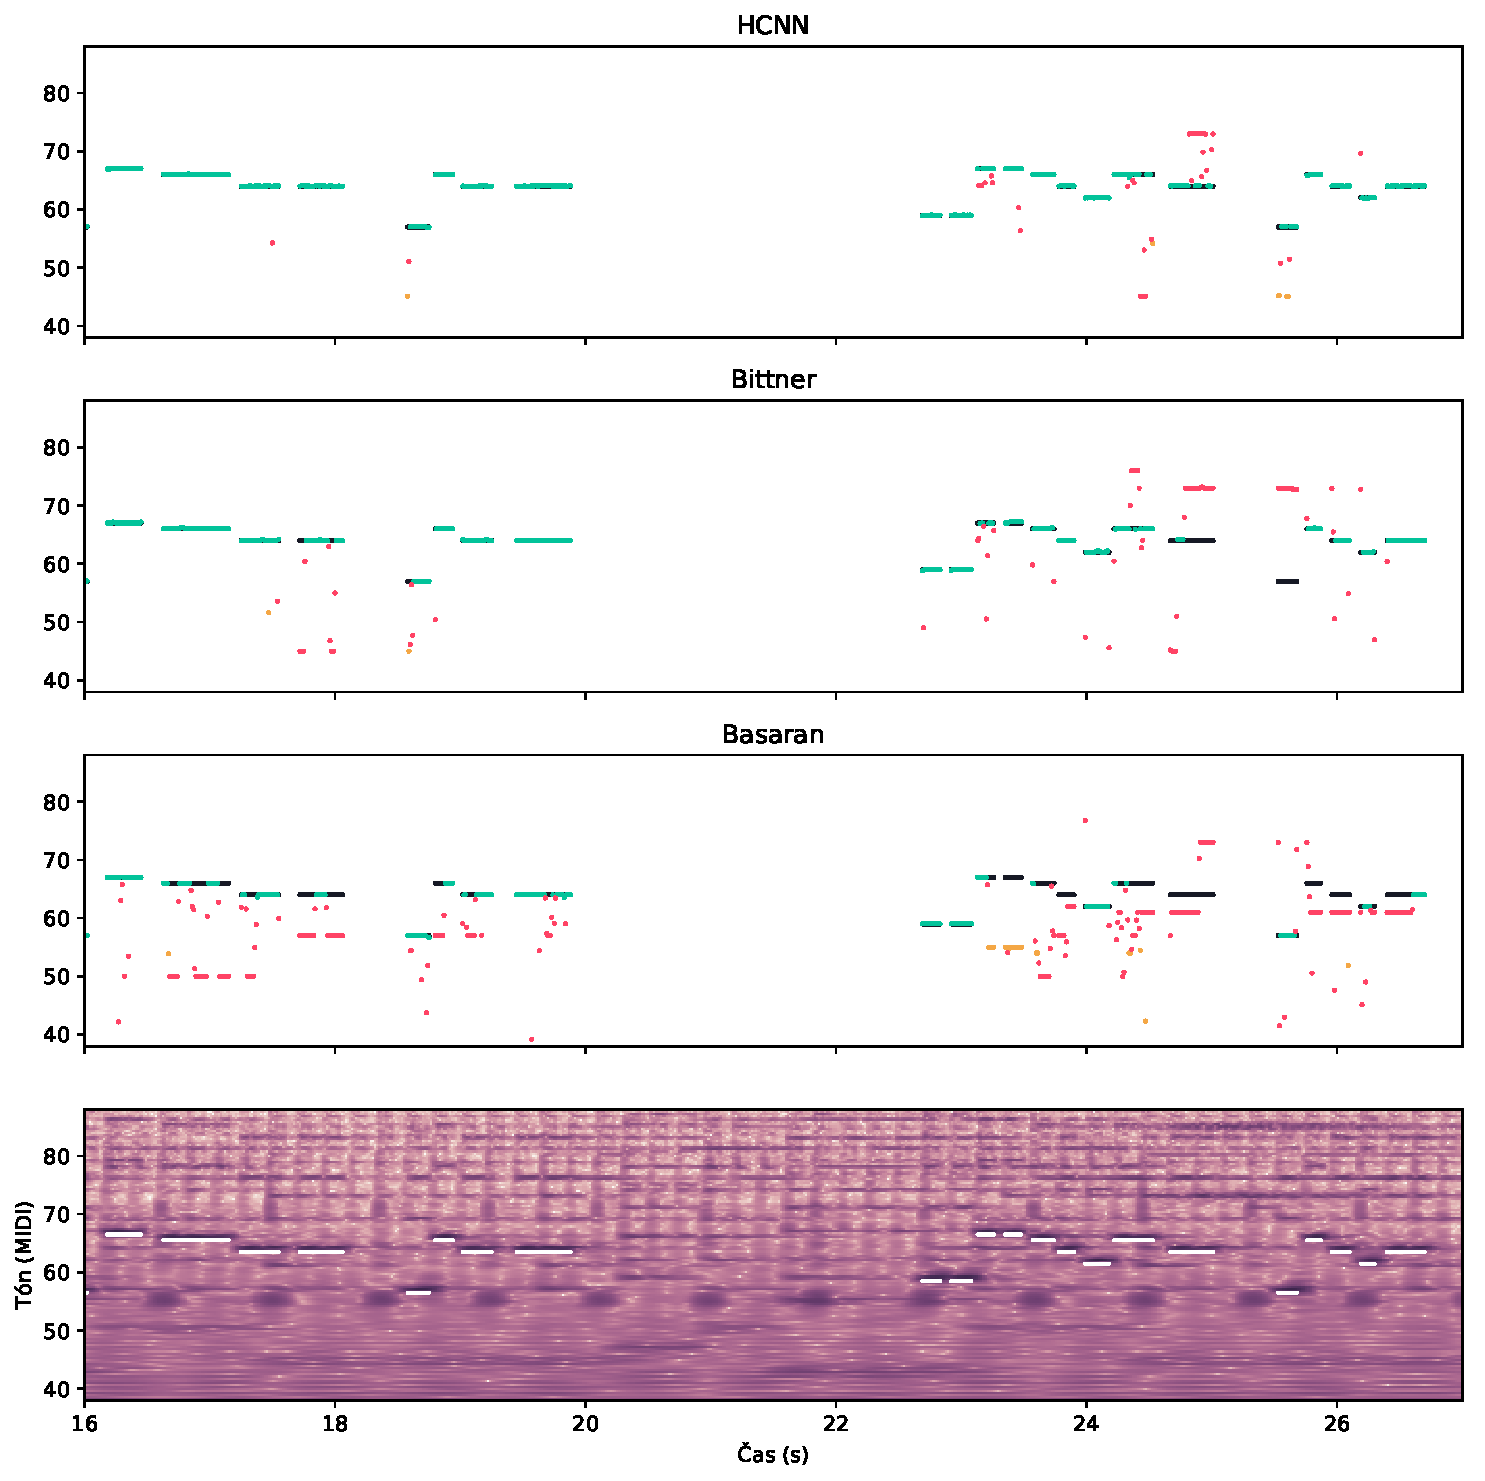
\includegraphics[width=\textwidth,height=\textheight,keepaspectratio]{../img/vysledky/mirex05_train10}
\caption{Výstup metod na testovacím souboru \texttt{train10} z datasetu MIREX05.}
\label{obr:mirex05_train10}
\end{figure}

\begin{figure}[p]\centering
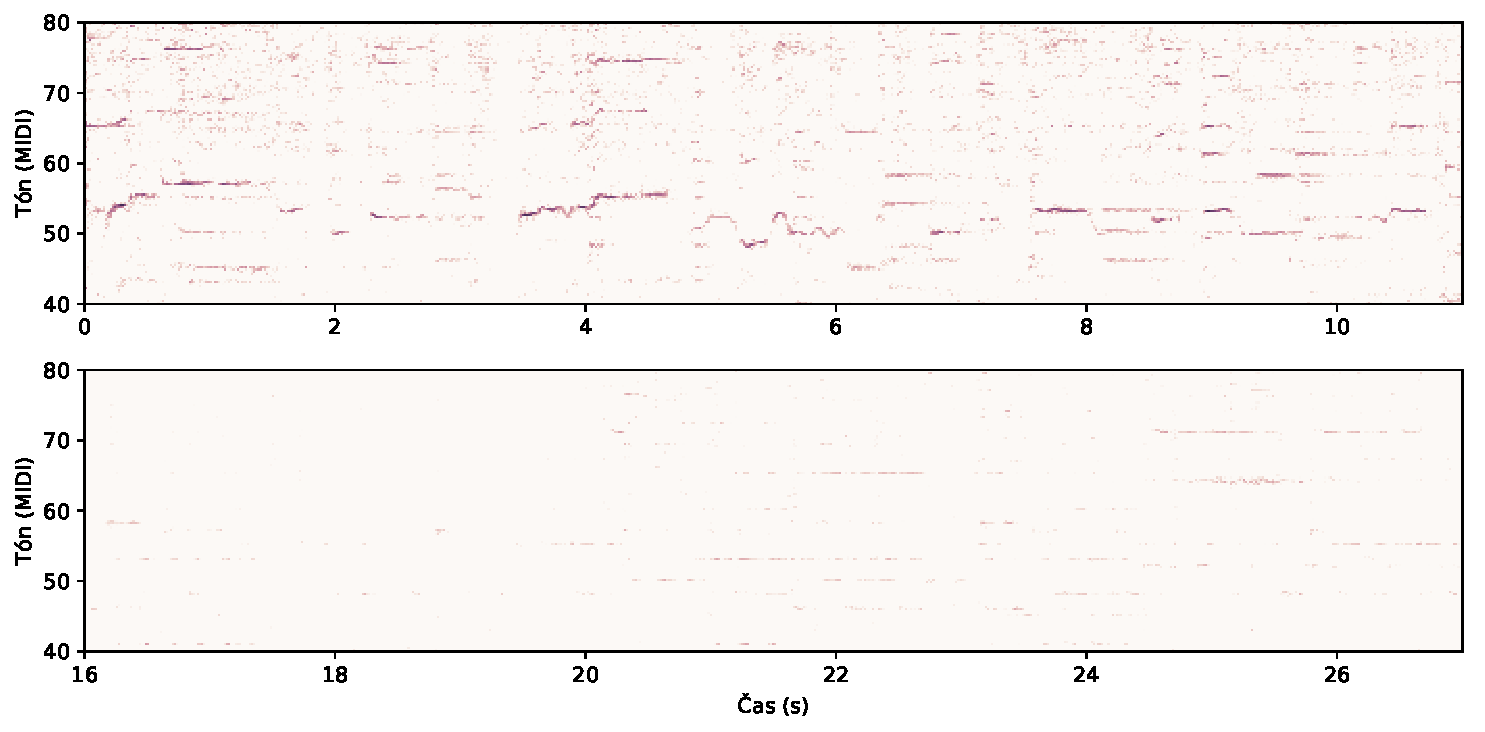
\includegraphics[width=\textwidth,height=\textheight,keepaspectratio]{../img/vysledky/basaran_salience_comparison}
\caption{Srovnání vstupní frekvenčně-časové reprezentace $\bm{\mathrm{H}}^{F_0}$ Basaranovy metody testovacích souborů \texttt{train01} a \texttt{train10} z datasetu MIREX05.}
\label{obr:basaran_salience_comparison}
\end{figure}
Dalším problémem Basaranovy metody je zhoršená schopnost extrakce na syntetických datech. Příklady \texttt{midi2REF}, \texttt{midi3REF}, \texttt{train10REF} z datasetů ADC04 a MIREX05 jsou syntetizovány na základě MIDI pomocí základních zvukových fontů, nahrávky proto zní velmi uměle. Jak vidíme na obrázku \ref{obr:mirex05_train10}, zatímco metody Bittnerové a HCNN si s touto syntetickou barvou hlasu dokáží poradit, výstup Basaranovy metody obsahuje šum a skoky k doprovázejícím nástrojům. Příčinou může být jiná vstupní reprezentace signálu, která je založena na práci \cite{Durrieu2010} a spočívá na modelování hlavního hlasu pomocí zdroje a filtrů. Na obrázku \ref{obr:basaran_salience_comparison} srovnáváme tuto reprezentaci pro vstupní signál s lidským zpěvem (nahoře, \texttt{train01}) a pro signál se syntetickou flétnou (dole, \texttt{train10}). Je zřejmé, že zatímco lidský zpěv tato reprezntace dokáže zachytit, syntetický hlas na reprezentaci téměř zachycen není. 

\begin{figure}[h]\centering
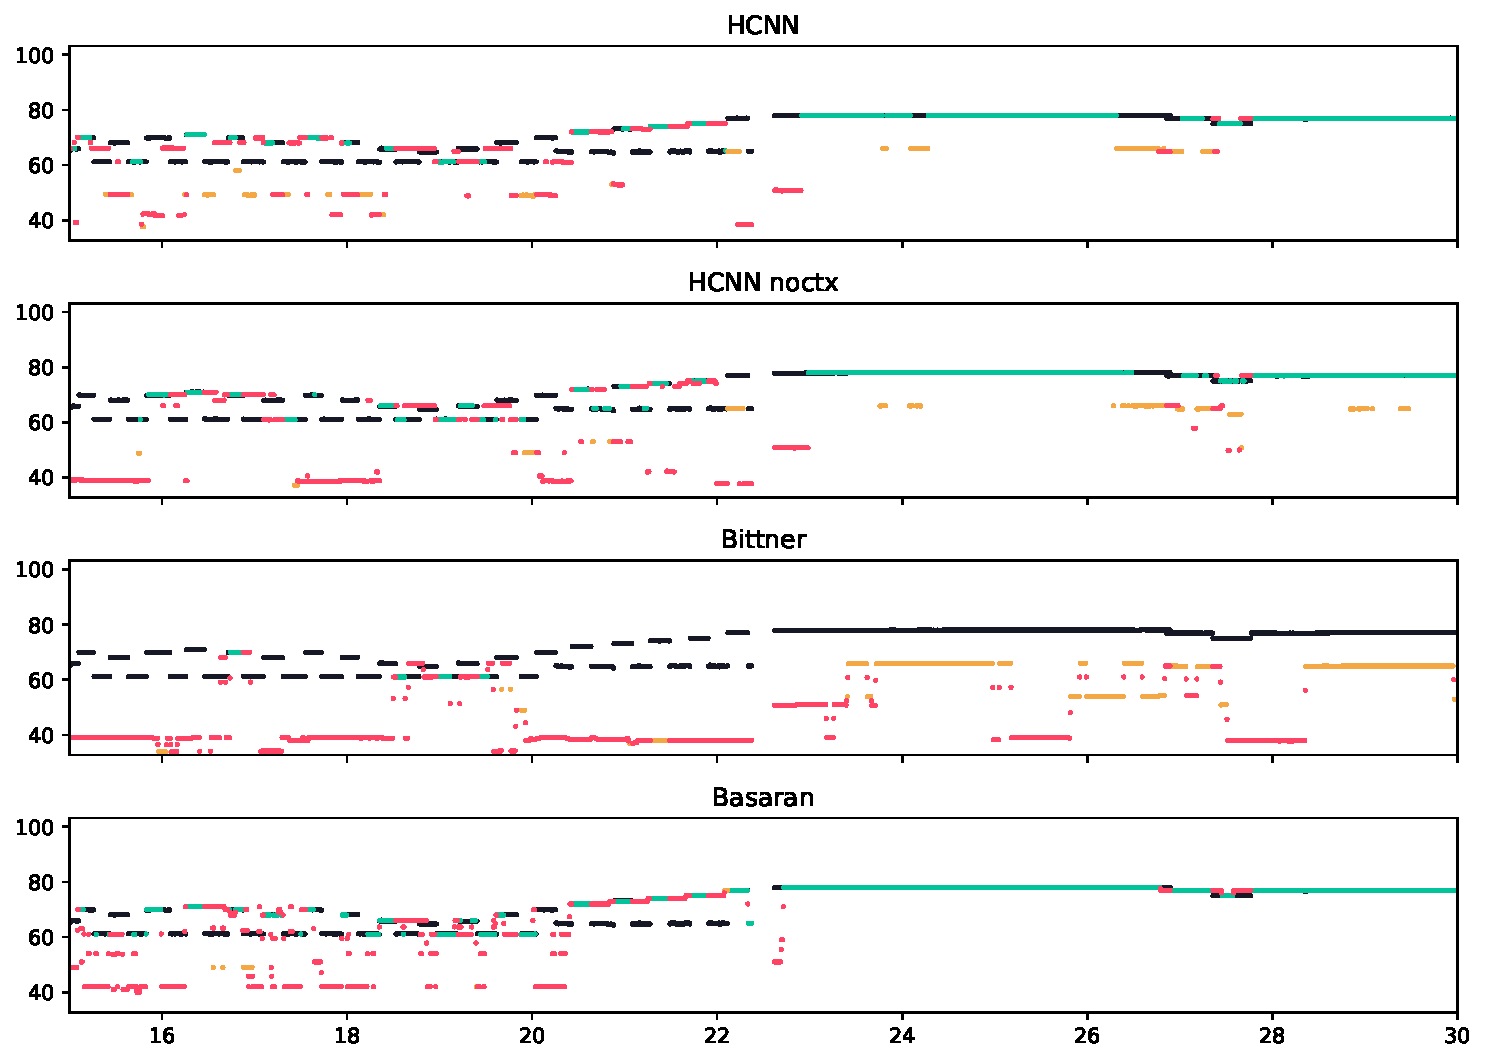
\includegraphics[width=\textwidth,height=\textheight,keepaspectratio]{../img/vysledky/mdb_MatthewEntwistle_FairerHopes}
\caption{Výstup metod na testovacím souboru \texttt{Matthew\allowbreak{}Entwistle\allowbreak{}\_Fairer\allowbreak{}Hopes} z datasetu MedleyDB.}
\label{obr:mdb_MatthewEntwistle_FairerHopes}
\end{figure}
Pokud srovnáme metody HCNN a metodu Bittner, rozdílem v predikcích jsou zejména jiné priority, které přiřazují barvám hlasů. Lze tudíž nalézt mnoho příkladů, kde HCNN zároveň přepisuje melodii a nesprávně místy přeskakuje k nástrojům v doprovodu, zatímco metoda Bittnerové na stejném příkladu tuto chybu nedělá, podobně však existují i opačné příklady. Příkladem, ve kterém se tyto metody nejvíce rozchází, je soubor \texttt{MatthewEntwistle\_FairerHopes} z kolekce MedleyDB, ve kterém melodii hraje harfa. Zvuk harfy se však nevyskytuje v množině trénovacích dat, rozdílem proto je, že zatímco metoda HCNN zvládá alespoň částečně generalizovat i na tuto dosud neslyšenou barvu hlasu, metoda Bittnerové tyto tóny úplně ignoruje a přepisuje doprovod pod harfou (viz obrázek \ref{obr:mdb_MatthewEntwistle_FairerHopes}).

\section{Interpretace výsledků}

Zásadní výhodou metody Basaran oproti HCNN a Bittner je zpracování výsledků funkce salience pomocí rekuretní sítě. Tento rozdíl spolu s jinou výchozí časově-frekvenční reprezentací signálu jeho metodu zvýhodňuje zejména na datasetu ORCHSET, kde jeho metoda v metrice RPA dosahuje o deset procentních bodů lepších výsledků. Pro metodu Basaran je na tomto datasetu také výhodné, že jeho referenční anotace mají půltónové frekvenční rozlišení, tedy stejné, jako výstup této metody. Tudíž jeho metoda při použití tohoto hrubého rozlišení nijak netratí. Na zbylých datasetech se však nižší frekvenční rozlišení projevuje více a metodu pravděpodobně spíše znevýhodňuje. Přesto jsou jeho predikce, zejména pak na složitějších vstupních datech, často koherentnější, obsahují méně šumu. 

Výsledky HCNN a Bittner jsou si oproti výsledkům metody Basaran mnohem podobnější, ačkoliv je mezi nimi větší procentuální rozdíl. Při kvalitativním vyhodnocování jsme nenalezli příliš mnoho příkladů, na kterém by se výstupy metod výrazně lišily. Mezi sítěmi je však řada podobností, zejména stejná vstupní reprezentace, přibližně stejně velký zpracovávaný kontext, přeskočení vyhlazování výstupu ale i celková struktura sítě. Kvantitativní rozdíly na všech datasetech tedy přičítáme spíše lépe naučeným barvám nástrojů a jejich priorit v celkovém mixu. Podobnost výsledků ilustrujeme také výpočtem korelace, zatímco výsledky metriky RPA pro metody Bittner a HCNN mezi sebou mají korelaci 0.932, mezi Basaran a HCNN vychází nižší korelace 0.736.

\section{Online demo}

Pro kvalitativní srovnání výsledků všech metod představovaných v práci je zpřístupněno jednoduché online demo na url \url{http://jirkabalhar.cz:6090/}. 

% \begin{table}[h!]
% \centering

%   \begin{tabular}{ll}
%   \toprule
%   Metrika (Metoda) & MatthewEntwistle\_FairerHopes \\
%   \midrule
%         RPA (HCNN) &                        0.451 \\
%         RCA (HCNN) &                        0.626 \\
%     RPA (Bittner) &                        0.118 \\
%     RCA (Bittner) &                        0.423 \\
%     RPA (Basaran) &                        0.544 \\
%     RCA (Basaran) &                        0.661 \\
%   \bottomrule
%   \end{tabular}

% \caption{Přesnost metod na testovacím souboru \texttt{MatthewEntwistle\_FairerHopes} z datasetu MedleyDB.}\label{tab:mdb_MatthewEntwistle_FairerHopes}
% \end{table}




% \begin{figure}[h]\centering
% 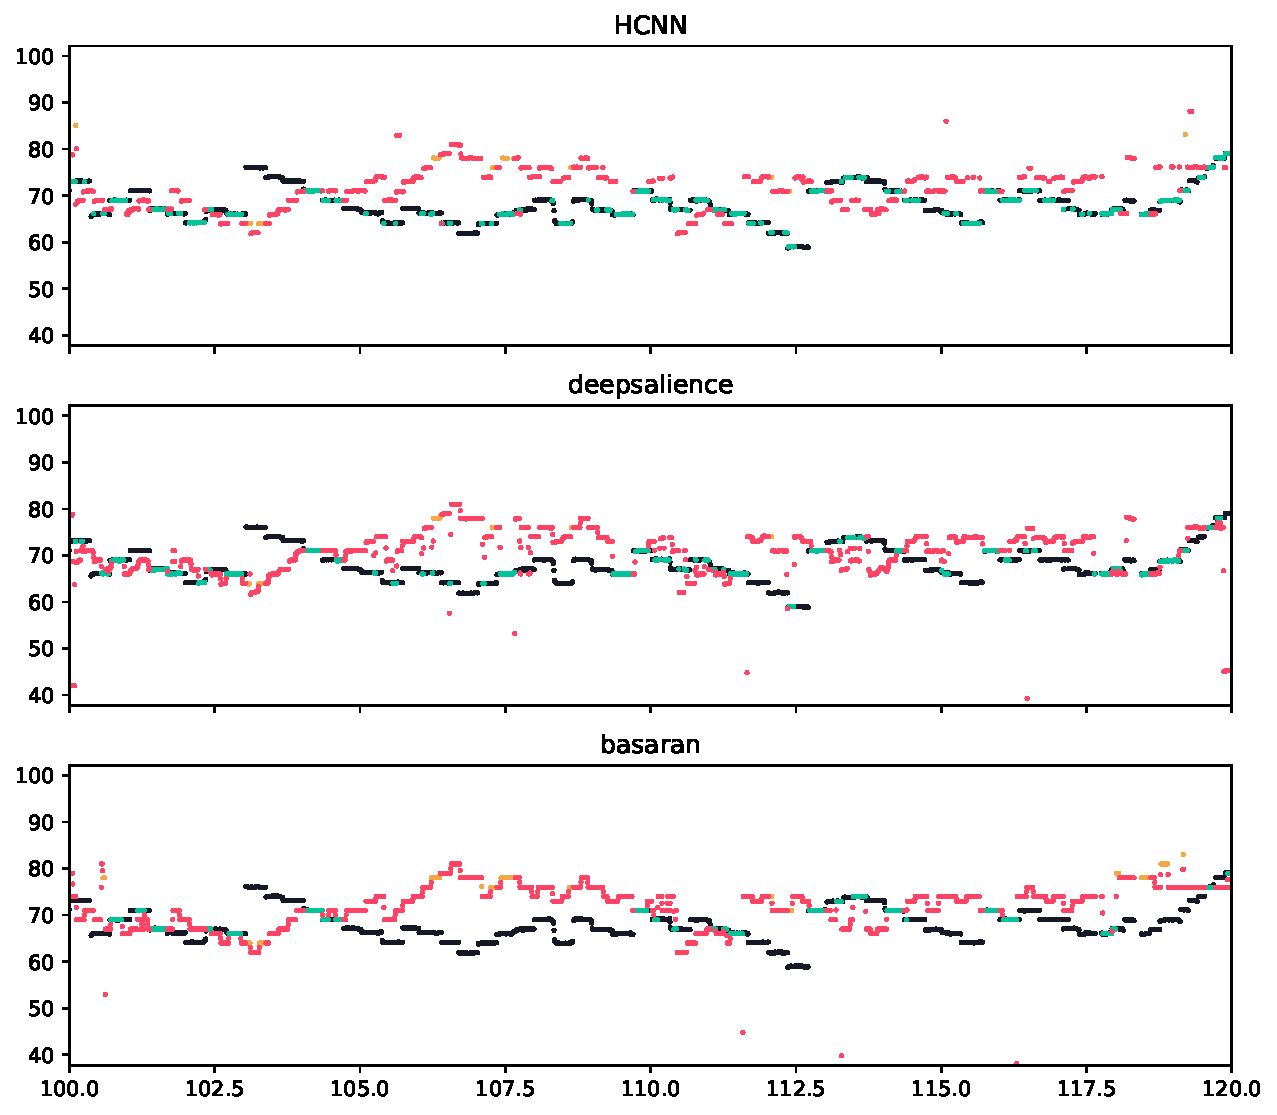
\includegraphics[width=\textwidth,height=\textheight,keepaspectratio]{../img/vysledky/mdb_MusicDelta_Pachelbel}
% \caption{Výstup metod na testovacím souboru \texttt{MusicDelta\_Pachelbel} z datasetu MedleyDB.}
% \label{obr:mdb_MusicDelta_Pachelbel}
% \end{figure}

% \begin{table}[h!]
% \centering

% \begin{tabular}{ll}
% \toprule
% Metrika (Metoda) & MusicDelta\_Pachelbel \\
% \midrule
%       RPA (HCNN) &                0.472 \\
%       RCA (HCNN) &                0.510 \\
%    RPA (Bittner) &                0.461 \\
%    RCA (Bittner) &                0.493 \\
%    RPA (Basaran) &                0.435 \\
%    RCA (Basaran) &                0.491 \\
% \bottomrule
% \end{tabular}

% \caption{Přesnost metod na testovacím souboru \texttt{MusicDelta\_Pachelbel} z datasetu MedleyDB.}\label{tab:mdb_MusicDelta_Pachelbel}
% \end{table}


\chapter*{Závěr}
\addcontentsline{toc}{chapter}{Závěr}

% V práci prezentujeme tři nové metody výpočtu funkce salience s důrazem na odhad výšky tónů v nahrávkách. Ze tří navrhovaných dosáhla architektura HCNN výsledků, které na většině veřejně dostupných datasetech překonávají state-of-the-art metody extrakce melodie. 

%%% Seznam použité literatury
%%% Seznam použité literatury (bibliografie)
%%%
%%% Pro vytváření bibliografie používáme bibTeX. Ten zpracovává
%%% citace v textu (např. makro \cite{...}) a vyhledává k nim literaturu
%%% v souboru literatura.bib.
%%%
%%% Příkaz \bibliographystyle určuje, jakým stylem budou citovány odkazy
%%% v textu. V závorce je název zvoleného souboru .bst. Styly plainnat
%%% a unsrt jsou standardní součástí latexových distribucí. Styl czplainnat
%%% je dodáván s touto šablonou a bibTeX ho hledá v aktuálním adresáři.

\bibliographystyle{czplainnat}    %% Autor (rok) s českými spojkami
% \bibliographystyle{plainnat}    %% Autor (rok) s anglickými spojkami
% \bibliographystyle{unsrt}       %% [číslo]

\renewcommand{\bibname}{Seznam použité literatury}

%%% Vytvoření seznamu literatury. Pozor, pokud jste necitovali ani jednu
%%% položku, seznam se automaticky vynechá.

\bibliography{library}

%%% Kdybyste chtěli bibliografii vytvářet ručně (bez bibTeXu), lze to udělat
%%% následovně. V takovém případě se řiďte normou ISO 690 a zvyklostmi v oboru.

% \begin{thebibliography}{99}
%
% \bibitem{lamport94}
%   {\sc Lamport,} Leslie.
%   \emph{\LaTeX: A Document Preparation System}.
%   2. vydání.
%   Massachusetts: Addison Wesley, 1994.
%   ISBN 0-201-52983-1.
%
% \end{thebibliography}


%%% Obrázky v bakalářské práci
%%% (pokud jich je malé množství, obvykle není třeba seznam uvádět)
\listoffigures

%%% Tabulky v bakalářské práci (opět nemusí být nutné uvádět)
%%% U matematických prací může být lepší přemístit seznam tabulek na začátek práce.
\listoftables

%%% Použité zkratky v bakalářské práci (opět nemusí být nutné uvádět)
%%% U matematických prací může být lepší přemístit seznam zkratek na začátek práce.
\chapwithtoc{Seznam použitých zkratek}

\begin{tabular}{ll}
MIDI & Musical Instrument Digital Interface \\
MIR & Music Information Retrieval \\
MIREX & Music Information Retrieval Evaluation eXchange \\
ISMIR & The International Society of Music Information Retrieval \\
OA & Overall Accuracy \\
RPA & Raw Pitch Accuracy \\
RCA & Raw Chroma Accuracy \\
VR & Voicing Recall \\
VFA & Voicing False Alarm \\
HCQT & Harmonic Constant-Q Transform \\
CQT & Constant-Q Transform \\
STFT & Short Time Fourier Transform \\
FFT & Fast Fourier Transform \\
HCNN & Harmonic Convolutional Neural Network \\
\end{tabular}

%%% Přílohy k bakalářské práci, existují-li. Každá příloha musí být alespoň jednou
%%% odkazována z vlastního textu práce. Přílohy se číslují.
%%%
%%% Do tištěné verze se spíše hodí přílohy, které lze číst a prohlížet (dodatečné
%%% tabulky a grafy, různé textové doplňky, ukázky výstupů z počítačových programů,
%%% apod.). Do elektronické verze se hodí přílohy, které budou spíše používány
%%% v elektronické podobě než čteny (zdrojové kódy programů, datové soubory,
%%% interaktivní grafy apod.). Elektronické přílohy se nahrávají do SISu a lze
%%% je také do práce vložit na CD/DVD. Povolené formáty souborů specifikuje
%%% opatření rektora č. 23/2016.
\chapwithtoc{Přílohy}

% \appendix
% \chapter{Přílohy}

\section{Architektura HCNN, Vliv úpravy architektury ovlivňující receptivní pole modelu}\label{appendix:hcnn_ctx}

\begin{table}[h]
\centering
\scalebox{0.90}{%
\begin{tabular}{llrr}

\toprule
Konfigurace bloků & Úprava architektury &   RPA &   RCA \\
\midrule
8 filtrů, 4 konv. bloky & noctx & 0.722 & 0.786 \\
{} & deep\_ctx\_3 & 0.728 & 0.796 \\
{} & first\_layers\_ctx & 0.728 & 0.795 \\
{} & last\_layers\_ctx & 0.737 & 0.800 \\
{} & 1\_last\_layer\_dilated & 0.733 & 0.797 \\
{} & 2\_last\_layers\_dilated & 0.733 & 0.796 \\
{} & 3\_last\_layers\_dilated & 0.731 & 0.796 \\
{} & 2\_last\_layers\_wavenet & 0.733 & 0.798 \\
{} & 3\_last\_layers\_wavenet & 0.745 & 0.804 \\
\arrayrulecolor{black!30}\midrule
16 filtrů, 4 konv. bloky & noctx & 0.737 & 0.802 \\
{} & deep\_ctx\_3 & 0.744 & 0.806 \\
{} & first\_layers\_ctx & 0.744 & 0.804 \\
{} & last\_layers\_ctx & 0.757 & 0.817 \\
{} & 1\_last\_layer\_dilated & 0.743 & 0.802 \\
{} & 2\_last\_layers\_dilated & 0.749 & 0.814 \\
{} & 3\_last\_layers\_dilated & 0.752 & 0.813 \\
{} & 2\_last\_layers\_wavenet & 0.754 & 0.813 \\
{} & 3\_last\_layers\_wavenet & 0.761 & 0.819 \\
\arrayrulecolor{black!30}\midrule
8 filtrů, 8 konv. bloků & noctx & 0.732 & 0.801 \\
{} & deep\_ctx\_3 & 0.735 & 0.796 \\
{} & first\_layers\_ctx & 0.747 & 0.814 \\
{} & last\_layers\_ctx & 0.749 & 0.811 \\
{} & 1\_last\_layer\_dilated & 0.745 & 0.806 \\
{} & 2\_last\_layers\_dilated & 0.751 & 0.814 \\
{} & 3\_last\_layers\_dilated & 0.749 & 0.806 \\
{} & 2\_last\_layers\_wavenet & 0.754 & 0.814 \\
{} & 3\_last\_layers\_wavenet & 0.751 & 0.803 \\
\arrayrulecolor{black!30}\midrule
16 filtrů, 8 konv. bloků & noctx & 0.744 & 0.809 \\
{} & deep\_ctx\_3 & 0.741 & 0.815 \\
{} & first\_layers\_ctx & 0.748 & 0.817 \\
{} & last\_layers\_ctx & 0.749 & 0.819 \\
{} & 1\_last\_layer\_dilated & 0.753 & 0.817 \\
{} & 2\_last\_layers\_dilated & 0.758 & 0.819 \\
{} & 3\_last\_layers\_dilated & 0.757 & 0.817 \\
{} & 2\_last\_layers\_wavenet & 0.759 & 0.819 \\
{} & 3\_last\_layers\_wavenet & 0.749 & 0.809 \\
\arrayrulecolor{black}\bottomrule
\end{tabular}
}%
\caption{Architektura HCNN, Vliv úpravy architektury ovlivňující receptivní pole modelu.}\label{tab:spectrogram_ctx_archs}
\end{table}

\openright
\end{document}
